    %==============================================================================
    % LIBRO DE PROYECTO DE GRADO - UIS
    % Implementación y análisis del desempeño de un pipeline para el estudio de %amplicones 16S en un clúster energéticamente eficiente basado en Raspberry Pi 5
    %==============================================================================
    
    \documentclass[12pt,oneside,spanish]{book}
    
    %==============================================================================
    % PAQUETES
    %==============================================================================
    
    \usepackage[utf8]{inputenc}
    \usepackage[T1]{fontenc}
    \usepackage[spanish,es-tabla,es-noshorthands]{babel}
    \usepackage[margin=2.5cm]{geometry}
    \usepackage{setspace}
    \usepackage{fancyhdr}
    \usepackage{graphicx}
    \usepackage{booktabs}
    \usepackage{longtable}
    \usepackage{threeparttable}
    \usepackage{array}
    \usepackage{amsmath}
    \usepackage{amssymb}
    \usepackage{multirow}
    \usepackage[table]{xcolor}
    \usepackage{float}
    \usepackage{rotating}
    \usepackage{adjustbox}
    \usepackage[indent=2em]{parskip}
    \setlength{\emergencystretch}{2em}
    \usepackage[natbibapa]{apacite}
    \usepackage{xurl}
    \usepackage[hidelinks]{hyperref}
    
    
    %------------------------------------------------------------------------------
    
    %==============================================================================
    % CONFIGURACIÓN DE ESPACIADO
    %==============================================================================
    
    \onehalfspacing
    
    %==============================================================================
    % ENCABEZADOS Y PIES
    %==============================================================================
    
    \pagestyle{fancy}
    \fancyhf{}
    \fancyhead[R]{\thepage}
    \renewcommand{\headrulewidth}{0pt}
    \renewcommand{\footrulewidth}{0pt}
    \setlength{\headheight}{14.5pt}
    \addtolength{\topmargin}{-2.5pt}
    
    %==============================================================================
    % CONFIGURACIÓN DE HIPERENLACES
    %==============================================================================
    
    \hypersetup{
        colorlinks=true,
        linkcolor=black,
        citecolor=black,
        urlcolor=blue,
        pdftitle={Implementación y análisis del desempeño de un pipeline para el estudio de amplicones 16S en un clúster energéticamente eficiente basado en Raspberry Pi 5},
        pdfauthor={Cristian Alberto Solano Torres; Zamir Francisco Granados Peñaloza},
        pdfcreator={LaTeX with hyperref},
        pdfproducer={pdfTeX}
    }
    
    %==============================================================================
    % NUEVA DEFINICIÓN DE CAPÍTULOS Y SECCIONES
    %==============================================================================
    
    \renewcommand{\thechapter}{\arabic{chapter}}
    \renewcommand{\theequation}{\arabic{chapter}.\arabic{equation}}
    \renewcommand{\thefigure}{\arabic{chapter}.\arabic{figure}}
    \renewcommand{\thetable}{\arabic{chapter}.\arabic{table}}
    
    %==============================================================================
    % INICIO DEL DOCUMENTO
    %==============================================================================
    
    \begin{document}
    
    %==============================================================================
    % PORTADA
    %==============================================================================
    
    \begin{titlepage}
        \centering
        \vspace*{1cm}
    
        {\Large \textbf{Implementación y análisis del desempeño de un pipeline para el estudio de amplicones 16S en un clúster energéticamente eficiente basado en Raspberry Pi 5}}
    
        \vspace{2cm}
    
        {\large \textbf{Cristian Alberto Solano Torres} 2211906 - Ingeniería de Sistemas}
    
        {\large \textbf{Zamir Francisco Granados Peñaloza} 2211888 - Ingeniería de Sistemas}
    
        \vspace{2cm}
    
        {\large Trabajo de Grado para Optar el Título de Ingeniero de Sistemas}
    
        \vspace{2cm}
    
        {\large \textbf{Director}}
    
        {\large \textbf{Bernardo Andrés Benavides Arévalo.} PhD - Director}
    
        \vspace{\fill}
    
        {\large Universidad Industrial de Santander}
    
        {\large Facultad de Ingenierías Físico-Mecánicas}
    
        {\large Escuela de Ingeniería de Sistemas e Informática}
    
        {\large Bucaramanga}
    
        {\large 2026}
    
    \end{titlepage}
    
    %==============================================================================
    % PÁGINA DE AGRADECIMIENTOS
    %==============================================================================
    
    \chapter*{Agradecimientos}
    \addcontentsline{toc}{chapter}{Agradecimientos}
    
    \vspace{1cm}
    
    Un sincero agradecimiento al director de este proyecto de grado, el profesor Bernardo Andrés Benavides Arévalo, por su acompañamiento durante el desarrollo de esta investigación. Su orientación técnica, sus observaciones y su disposición para discutir cada una de las decisiones que surgieron durante el proyecto fueron fundamentales para avanzar y superar los diferentes retos que encontramos en el camino. Agradecemos también la confianza que depositó en nosotros al permitirnos desarrollar un proyecto que nos llevó a explorar un campo interdisciplinario entre la ingeniería de sistemas y la bioinformática, y que representó una oportunidad para poner a prueba y fortalecer los conocimientos adquiridos durante nuestra formación.
    
    A la Escuela de Ingeniería de Sistemas e Informática y a la Universidad Industrial de Santander, por acompañarnos durante los años en los que construimos las bases de nuestra formación como ingenieros. Agradecemos los conocimientos, las experiencias y los espacios que nos permitieron aprender no solo a desarrollar soluciones desde la ingeniería, sino también a cuestionarlas, mejorarlas y asumir con responsabilidad los problemas que se presentan en nuestra profesión. Este proyecto representa, en buena medida, el resultado de todo ese proceso de aprendizaje y de los años que compartimos como estudiantes.
    
    \vspace{0.5cm}
    
    \noindent\textbf{Cristian Alberto Solano Torres}
    
    Agradezco especialmente a mis padres, Rosalba Torres Orejarena y Luis Alberto Solano Pinzón, por su amor, apoyo y confianza incondicional. Gracias por estar siempre a mi lado, por sostenerme en los momentos difíciles y, sobre todo, por no dejarme rendir cuando yo mismo llegué a pensar en hacerlo. Este logro también es de ustedes, porque detrás de cada paso que me trajo hasta aquí estuvieron su esfuerzo, sus consejos y la confianza que siempre depositaron en mí.A mis hermanas, Karen y Silvia, por estar pendientes de mí y acompañarme durante este proceso. Son ejemplos de superación y logro que me han ayudado a mantener presente mi objetivo en todo momento. Y a mi sobrina, Shara, por ser esa pequeña fuente de amor que ha mantenido unida a toda la familia y por tenerme presente en todos los pasos que da.
    
    A Zamir, mi compañero, por su esfuerzo y por dar ese impulso que muchas veces me hizo falta para seguir adelante. A Juan, mi mejor amigo, por ayudarme a mantener una actitud positiva y encontrar momentos de tranquilidad cuando todo parecía estar de cabeza, incluso después de aquellos momentos en los que estuvimos distanciados. Y a Daniel, por acompañarme cuando sentía que no podía salir de mis propios enredos y por ayudarme a encontrar claridad en esos momentos.
    
    Finalmente, quiero dedicar un recuerdo especial a mis abuelos, Abigail Orejarena de Torres y Noé Solano Rueda, quienes partieron durante estos años de formación y no pudieron acompañarme hasta este momento. Este logro también lleva una parte de ellos y de los recuerdos que dejaron en mi vida.
    
    \vspace{0.5cm}
    
    \noindent\textbf{Zamir Francisco Granados Peñaloza}
    
    Agradezco especialmente a mi familia. A mi madre, Patricia Peñaloza, quien me guio en cada paso y ha sido siempre mi consejera y mi refugio. A mis hermanos, Ronaldo, Heberth y Mabel, por acompañarme a lo largo de esta etapa con sus ocurrencias y con cada uno de sus favores. A Paula, mi compañera de vida, por comprenderme, apoyarme, escucharme y estar siempre para mí. A la memoria de Duke, mi amigo perruno, que me acompañó en los comienzos de este camino y me escuchaba en los momentos difíciles.
    
    A mi compañero Cristian, por ayudarme cuando algo de la universidad no me quedaba claro y por ser parte de este cierre. A mi amigo Jaider, por su apoyo y por ser una persona leal. A Yeison, por ser un amigo siempre dispuesto a ayudar. Y a mi amigo Rosemberg, que estuvo conmigo desde los inicios de mi carrera.
    
    A mi padre, Francisco Granados, mi mayor ejemplo de vida, mi inspiración y mi guía. Aunque ya no me acompañe en lo terrenal, sus enseñanzas me impulsan a seguir luchando por mis metas y sueños como el primer día. Este logro es por ustedes, mamá y papá, y lleva una parte de todos ustedes.
    
    
    %==============================================================================
    % RESUMEN
    %==============================================================================
    
    \chapter*{Resumen}
    \addcontentsline{toc}{chapter}{Resumen}
    
    \vspace{1cm}
    
    \noindent\textbf{Título:} Implementación y análisis del desempeño de un pipeline para el estudio de amplicones 16S en un clúster energéticamente eficiente basado en Raspberry Pi 5.
    
    \medskip
    
    \noindent\textbf{Autores:} Cristian Alberto Solano Torres; Zamir Francisco Granados Peñaloza.
    
    \medskip
    
    \noindent\textbf{Palabras Clave:} 16S rRNA; pipelines bioinformáticos; Raspberry Pi 5; ARM64; eficiencia energética; clúster de bajo consumo.
    
    \vspace{0.5cm}
    
    El análisis bioinformático de amplicones del gen 16S rRNA es una herramienta ampliamente utilizada en estudios de diversidad microbiana, genómica ambiental y diagnóstico molecular. Sin embargo, sus etapas de control de calidad, filtrado, inferencia de variantes y asignación taxonómica se ejecutan tradicionalmente sobre estaciones de trabajo o sistemas de computación de alto rendimiento (HPC) con un elevado consumo energético, lo que limita su uso en lugares con infraestructura reducida. En este trabajo se diseñó y construyó un clúster basado en microcomputadores Raspberry Pi 5 con arquitectura ARM64 y sistema operativo Ubuntu Server 24.04, sobre el cual se portaron y ejecutaron tres pipelines bioinformáticos (Kraken 2, LotuS3 y QIIME 2) para el análisis de amplicones 16S. El desempeño energético y computacional del clúster se comparó con el de dos computadores portátiles de arquitectura x86 con el mismo procesador, uno con Ubuntu 24.04 LTS nativo y otro con Ubuntu 22.04 LTS sobre el subsistema Windows Subsystem for Linux (WSL2), midiendo el tiempo de ejecución, el uso de CPU y memoria RAM y el consumo energético, a partir de los cuales se calculó la eficiencia energética expresada en lecturas procesadas (reads)  por vatio-hora (reads/Wh). Los resultados demostraron que los tres pipelines se ejecutaron exitosamente en el clúster ARM64 y preservaron la concordancia taxonómica frente a la plataforma x86 de referencia: en QIIME 2, las tablas de asignación taxonómica fueron 100\,\% idénticas, en Kraken 2 la concordancia de abundancias superó el 99.8\,\% y en LotuS3 las tres plataformas detectaron las mismas familias y los mismos géneros, con la misma puntuación F1 (F1-score). En cuanto al tiempo de ejecución, con las muestras repartidas en cinco nodos de cómputo el clúster fue 2.58$\times$ más rápido que la estación x86 nativa en QIIME 2, en LotuS3 se obtuvo un desempeño similar (0.96$\times$) y en Kraken 2 la estación x86 nativa fue 2.32$\times$ más rápida. Cabe resaltar que en Kraken2 y LotuS3 el tiempo del clúster quedó limitado por el almacenamiento de red compartido, desde el cual los cinco nodos leían la base de referencia al mismo tiempo. En términos de consumo energético, el clúster fue más eficiente que la estación x86 nativa en energía neta: 3.81$\times$ en Kraken 2, 2.14$\times$ en LotuS3 y 4.57$\times$ en QIIME 2. Como delimitaciones y limitaciones generales del proyecto se identifican las siguientes: Todos los experimentos se realizaron con secuencias sintéticas simuladas por la plataforma LEMMI16s para tener control sobre los resultados biológicos (\textit{Ground Truth}). Mientras que Kraken2 y QIIME2 operaron con sus clasificadores nativos basados en $k$-meros y Naive Bayes respectivamente, en LotuS3 la asignación taxonómica se realizó mediante el software VSEARCH para asegurar la reproducibilidad cruzada frente a la arquitectura ARM64. La memoria física disponible (16~GB por nodo) obligó a acotar la base taxonómica SILVA en QIIME 2 a las regiones V1--V2 para prevenir desbordamientos de memoria (OOM), descartando la clasificación contra bases globales completas sin reducción. El enlace Gigabit Ethernet y el almacenamiento NFS compartidos impusieron cuellos de botella de I/O en tareas de alta transferencia, como en Kraken 2 y LotuS3. Sin embargo, los resultados obtenidos en este estudio demuestran la viabilidad técnica, la reproducibilidad biológica y el potencial de eficiencia energética de las microarquitecturas ARM64 para una bioinformática accesible y de bajo costo.
    
    
    %==============================================================================
    % ABSTRACT
    %==============================================================================
    
    \chapter*{Abstract}
    \addcontentsline{toc}{chapter}{Abstract}
    
    \vspace{1cm}
    
    \noindent\textbf{Title:} Implementation and performance analysis of a pipeline for 16S amplicon studies on an energy-efficient cluster based on Raspberry Pi 5.
    
    \medskip
    
    \noindent\textbf{Authors:} Cristian Alberto Solano Torres; Zamir Francisco Granados Peñaloza.
    
    \medskip
    
    \noindent\textbf{Keywords:} 16S rRNA; bioinformatics pipelines; Raspberry Pi 5; ARM64; energy efficiency; low-power cluster.
    
    \vspace{0.5cm}
    
    Bioinformatic analysis of 16S rRNA gene amplicons is a widely used tool in microbial diversity studies, environmental genomics, and molecular diagnostics. However, its quality control, filtering, variant inference, and taxonomic assignment stages are traditionally executed on workstations or high-performance computing (HPC) systems with high energy consumption, which limits their use in locations with reduced infrastructure. In this work, a cluster based on Raspberry Pi 5 single-board computers with ARM64 architecture and Ubuntu Server 24.04 operating system was designed and built, on which three bioinformatic pipelines (Kraken 2, LotuS3, and QIIME 2) were ported and executed for 16S amplicon analysis. The energetic and computational performance of the cluster was compared with that of two x86 architecture laptop computers with the same processor, one with native Ubuntu 24.04 LTS and the other with Ubuntu 22.04 LTS on the Windows Subsystem for Linux (WSL2), measuring execution time, CPU and RAM usage, and energy consumption, from which energy efficiency was calculated, expressed in processed reads (reads) per watt-hour (reads/Wh). The results demonstrated that the three pipelines executed successfully on the ARM64 cluster and preserved taxonomic concordance compared to the reference x86 platform: in QIIME 2, the taxonomic assignment tables were 100\,\% identical, in Kraken 2 the abundance concordance exceeded 99.8\,\%, and in LotuS3 the three platforms detected the same families and the same genera, with the same F1 score (F1-score). Regarding execution time, with the samples distributed across five compute nodes, the cluster was 2.58$\times$ faster than the native x86 station in QIIME 2, in LotuS3 a similar performance was obtained (0.96$\times$), and in Kraken 2 the native x86 station was 2.32$\times$ faster. It should be noted that in Kraken 2 and LotuS3, the cluster's time was limited by the shared network storage, from which the five nodes read the reference database at the same time. In terms of energy consumption, the cluster was more efficient than the native x86 station in net energy: 3.81$\times$ in Kraken 2, 2.14$\times$ in LotuS3, and 4.57$\times$ in QIIME 2. As general delimitations and limitations of the project, the following are identified. All experiments were performed with synthetic sequences simulated by the LEMMI16s platform to have control over the biological results (\textit{Ground Truth}). While Kraken 2 and QIIME 2 operated with their native classifiers based on $k$-mers and Naive Bayes respectively, in LotuS3 taxonomic assignment was performed using the VSEARCH software to ensure cross-reproducibility against the ARM64 architecture. The available physical memory (16~GB per node) required restricting the SILVA taxonomic database in QIIME 2 to the V1--V2 regions to prevent out-of-memory (OOM) errors, ruling out classification against complete global databases without reduction. The shared Gigabit Ethernet link and NFS storage imposed I/O bottlenecks in high-transfer tasks, as in Kraken 2 and LotuS3. However, the results obtained in this study demonstrate the technical viability, biological reproducibility, and energy efficiency potential of ARM64 microarchitectures for accessible and low-cost bioinformatics.
    
    %==============================================================================
    % TABLA DE CONTENIDOS
    %==============================================================================
    
    \clearpage
    \tableofcontents
    
    %==============================================================================
    % LISTA DE TABLAS
    %==============================================================================
    
    \clearpage
    \listoftables
    
    %==============================================================================
    % LISTA DE FIGURAS
    %==============================================================================
    
    \clearpage
    \listoffigures
    
    %==============================================================================
    % GLOSARIO
    %==============================================================================
    
    \chapter*{Glosario}
    \addcontentsline{toc}{chapter}{Glosario}
    
    A continuación se definen los términos principales utilizados a lo largo del documento.
    
    \begin{description}
        \item[16S rRNA:] gen que codifica el RNA ribosomal en procariotas. Gracias a sus regiones conservadas e hipervariables, actúa como el principal marcador para la identificación y clasificación de bacterias.
        \item[Amplicón:] fragmento de DNA o RNA que es el producto directo de un evento de amplificación. Es la secuencia base para identificar la diversidad microbiana en este estudio.
        
        \item[ARM64:] arquitectura de procesador de 64 bits basada en un conjunto reducido de instrucciones. Su principal ventaja frente a arquitecturas tradicionales es que ofrece un rendimiento competitivo con un consumo de energía significativamente menor.
        
        \item[ASV (\textit{Amplicon Sequence Variant}):] variante exacta de una secuencia de amplicón, inferida con precisión de un solo nucleótido. Permite distinguir microorganismos con mayor resolución que los métodos tradicionales de agrupamiento
        
        \item[Clúster:] conjunto de computadores interconectados que trabajan de manera coordinada como si fueran un solo sistema. Permite distribuir tareas pesadas entre varios nodos para reducir el tiempo de procesamiento.
        
        \item[Green HPC (cómputo verde):] enfoque de la computación de alto rendimiento que busca maximizar el trabajo realizado por unidad de energía consumida, priorizando hardware y configuraciones de bajo consumo eléctrico.
        \item[HPC (\textit{High Performance Computing}):] computación de alto rendimiento. Hace referencia a sistemas con gran capacidad de cómputo, como supercomputadores o servidores especializados, típicamente usados en investigación científica, pero con alto consumo energético.
        
        \item[\textit{k}-mer:] fragmento de longitud fija extraído de una secuencia de DNA. Las herramientas bioinformáticas los usan para comparar secuencias rápidamente contra bases de datos e identificar qué organismos están presentes en una muestra.
        
        \item[OTU (\textit{Operational Taxonomic Unit}):] agrupamiento de secuencias de DNA con alta similitud entre sí, usado como unidad práctica para representar especies o grupos de microorganismos en estudios de diversidad microbiana.
        
        \item[Pipeline bioinformático:] sucesión automatizada de algoritmos y herramientas de software diseñadas para procesar datos biológicos crudos, filtrarlos y convertirlos en información analizable.
        
        \item[reads/Wh:] métrica de eficiencia energética que indica cuántas lecturas de secuenciación procesa un sistema por cada vatio-hora de energía consumida. A mayor valor, más eficiente es el sistema.
        
        \item[SBC (\textit{Single Board Computer}):] computador completo contenido en una sola placa de circuito impreso. Son dispositivos compactos, económicos y de bajo consumo, como la Raspberry Pi 5 utilizada en este proyecto.
        
        \item[Six Sigma (DMAIC):] metodología de mejora continua orientada a la reducción de variabilidad y la optimización del rendimiento, adaptada aquí para la validación y mejora de sistemas computacionales. Sus etapas son Definir, Medir, Analizar, Mejorar y Controlar.
        
        \item[WSL2 (\textit{Windows Subsystem for Linux 2}):] capa de compatibilidad de Windows que ejecuta un núcleo Linux real dentro de una máquina virtual ligera, permitiendo usar distribuciones como Ubuntu sin reemplazar el sistema operativo anfitrión.
    \end{description}
    
    %==============================================================================
    % INTRODUCCIÓN
    %==============================================================================
    
    \chapter*{Introducción}
    \addcontentsline{toc}{chapter}{Introducción}
    \setcounter{chapter}{0}
    \setcounter{equation}{0}
    \setcounter{figure}{0}
    \setcounter{table}{0}
    \setcounter{secnumdepth}{4} 
    \setcounter{tocdepth}{4}
    
    El gen 16S es un fragmento molecular del ácido desoxirribonucleico (DNA) utilizado para ayudar a identificar microorganismos, especialmente bacterias. La secuenciación de amplicones 16S es un método de laboratorio que usa pasos detallados y tecnologías específicas para capturarlo y representarlo en forma de archivo de texto, en formato FASTA o FASTQ \citep{cock2010fastq}. A partir de estos datos se realiza un análisis bioinformático que permite interpretar las secuencias obtenidas y que es ampliamente utilizado en estudios de diversidad microbiana, genómica ambiental y diagnóstico molecular \citep{clarridge2004}. Este tipo de análisis contiene diversas etapas, como control de calidad, filtrado de secuencias, inferencia de variantes y asignación taxonómica, las cuales requieren arquitecturas multinúcleo y multitarea, como estaciones de trabajo o sistemas HPC, que presentan un elevado consumo de energía. Por ejemplo, una estación de trabajo científica puede llegar a consumir entre 300 y 600~W, y un nodo de computación de alto rendimiento entre 300 y 5000~W \citep{cox2014iridis}. Estas restricciones dificultan el uso de dichas arquitecturas en lugares con infraestructura reducida y generan problemas de sostenibilidad energética.
    
    Gracias al avance tecnológico, actualmente es posible disponer de sistemas de cómputo basados en microordenadores, que permiten construir sistemas con menores prestaciones computacionales en comparación con una estación de trabajo o un sistema HPC, pero con un menor consumo energético \citep{pyrhonen2025energy}. En este proyecto se analizó el consumo energético de pipelines de análisis de amplicones 16S ejecutados sobre un clúster de computación basado en microcomputadores Raspberry Pi 5 (en adelante RBPi5). La elección de esta plataforma se justifica por su arquitectura ARM de 64 bits, su bajo consumo energético y su capacidad para soportar la ejecución de programas concurrentes. Los reportes de fábrica indican que, la RBPi5 se alimenta con una fuente de 5~V/5~A, equivalente a una potencia de 25~W por unidad \citep{rpi2023brief}.
    
    El objetivo de este proyecto fue implementar y evaluar pipelines bioinformáticos para el análisis de amplicones 16S, orientando su ejecución hacia infraestructuras más eficientes energéticamente. Para lograrlo, se construyó un clúster RBPi5 con Ubuntu Server 24.04 sobre el cual se portaron y ejecutaron tres pipelines, y se evaluó su comportamiento frente a dos computadores portátiles de arquitectura x86 (Intel) mediante métricas de tiempo de ejecución, demanda de recursos computacionales (CPU y RAM) y consumo energético, con el fin de analizar el balance entre desempeño y eficiencia energética, evaluada como el total de secuencias (\textit{reads}) analizadas por unidad de energía (reads/Wh).
    
    El documento se organiza de la siguiente manera: el Capítulo~\ref{cap:marco} presenta el marco de referencia, que incluye los fundamentos teóricos y el estado del arte. El Capítulo~\ref{cap:metodologia} describe la metodología y los entornos experimentales. El Capítulo~\ref{cap:resultados} presenta los resultados obtenidos en cada fase. Y el Capítulo~\ref{cap:conclusiones} expone las conclusiones y el trabajo futuro.
    
    %------------------------------------------------------------------------------
    % PLANTEAMIENTO Y JUSTIFICACIÓN DEL PROBLEMA
    %------------------------------------------------------------------------------
    
    \section*{Planteamiento y justificación del problema}
    \addcontentsline{toc}{section}{Planteamiento y justificación del problema}
    
    Los pipelines bioinformáticos para el análisis de amplicones 16S demandan recursos computacionales considerables. Herramientas como Kraken~2 \citep{wood2019kraken2, wood2024manual} pueden requerir entre 8 y 100~GB de memoria RAM según la base de datos empleada, mientras que DADA2 y QIIME~2 requieren entre 8 y 32~GB para conjuntos de datos moderados \citep{callahan2016dada2, bolyen2019qiime2}. A esto se suma la necesidad de almacenamiento para archivos FASTQ y bases de datos que pueden ocupar decenas o cientos de gigabytes. Por esta razón, su ejecución se ha concentrado tradicionalmente en infraestructuras robustas, como estaciones de trabajo multinúcleo y sistemas HPC \citep{seppey2025lemmi}, cuyo consumo eléctrico es elevado.
    
    Las alternativas de aceleración por hardware especializado, como GPU y FPGA, reducen los tiempos de procesamiento, pero su alto costo, su consumo energético y la complejidad de su configuración dificultan su adopción en entornos con recursos limitados \citep{robinson2021hardware}. Por otro lado, aunque los clústeres basados en arquitectura ARM han demostrado ser eficientes para diversas cargas científicas \citep{maqbool2015arm, warade2022}, en la literatura revisada no se encontraron reportes que validen la operatividad o el desempeño de la mayoría de los pipelines de análisis de amplicones 16S sobre arquitectura ARM64, y las implementaciones existentes en dispositivos de bajo consumo, como las de EPI2ME Labs, están orientadas principalmente al análisis metagenómico restringidos a tecnologías Oxford Nanopore \citep{ont2024wfmetagenomics}.
    
    En consecuencia, se hace necesario explorar plataformas accesibles, de bajo consumo y fácil implementación que puedan ejecutar análisis bioinformáticos de amplicones 16S, y cuantificar objetivamente su desempeño y eficiencia energética en plataformas de bajo consumo energético frente a las arquitecturas convencionales. Este proyecto muestra la implementación y evaluación de pipelines bioinformáticos en un clúster RBPi5, plataforma que combina la arquitectura ARM64 con un bajo consumo de energía y un costo mucho menor que el de las alternativas.
    
    En este contexto, el proyecto responde la siguiente pregunta de investigación:
    
    \vspace{0.5cm}
    
    \noindent\fbox{\parbox{\dimexpr\textwidth-2\fboxsep-2\fboxrule}{%
    \textbf{¿Cuál es la eficiencia energética y el rendimiento de procesamiento de un pipeline de análisis de amplicones 16S ejecutado en un clúster Raspberry Pi 5, frente a una estación de trabajo de arquitectura x86 estándar (total de secuencias analizadas por unidad de energía, reads/Wh)?}
    }}
    
    \vspace{0.5cm}
    
    %------------------------------------------------------------------------------
    % OBJETIVOS
    %------------------------------------------------------------------------------
    
    \section*{Objetivos}
    \addcontentsline{toc}{section}{Objetivos}
    
    \subsection*{Objetivo General}
    
    Analizar el desempeño y la eficiencia energética de un pipeline bioinformático para el estudio de amplicones 16S, ejecutado sobre un clúster de Raspberry Pi 5 frente a una estación de trabajo de arquitectura x86 estándar.
    
    \subsection*{Objetivos Específicos}
    
    \begin{enumerate}
        \item Diseñar la arquitectura hardware y software del clúster, definiendo la topología de red y los componentes necesarios para el despliegue del sistema bioinformático sobre arquitectura ARM64.
    
        \item Portar a la arquitectura ARM64 un pipeline bioinformático de análisis de 16S, permitiendo su ejecución en paralelo dentro del clúster.
    
        \item Validar la integridad funcional del pipeline mediante el procesamiento de conjuntos de datos de amplicones representativos, verificando que los resultados biológicos obtenidos en el clúster Raspberry Pi 5 sean consistentes y comparables con los generados en una arquitectura x86 estándar o similar.
    
        \item Evaluar el desempeño del sistema comparando métricas de tiempo de ejecución, uso de recursos (CPU y memoria) y consumo energético frente a una estación de trabajo de control, estableciendo la relación de eficiencia final en reads/Wh.
    \end{enumerate}
    
    %==============================================================================
    % CAPÍTULO 1: MARCO DE REFERENCIA
    %==============================================================================
    
    \chapter{Marco de referencia}
    \label{cap:marco}
    
    \section{Marco teórico}
    
    \subsection{El marcador 16S rRNA}
    
    El gen 16S rRNA (ácido ribonucleico ribosómico), mostrado en la Figura~\ref{fig:16s}, es parte del DNA ribosómico y se encuentra en todas las bacterias y arqueas. Se emplea extensamente como un marcador filogenético universal. Tiene una longitud aproximada de 1.500 pares de bases y presenta zonas con un alto grado de conservación, lo cual simplifica el diseño de marcadores universales. Entre estas zonas hay otras regiones llamadas hipervariables (V1 a V9), que tienen la suficiente variabilidad para permitir la distinción entre linajes de bacterias \citep{clarridge2004}. Todas estas características convierten al 16S rRNA en un marcador útil para estudiar la diversidad bacteriana y establecer relaciones filogenéticas entre microorganismos.
    
    \begin{figure}[H]
        \centering
        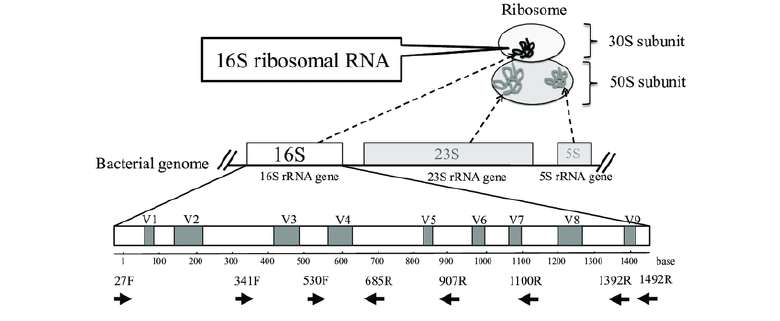
\includegraphics[width=0.85\textwidth]{figuras/estructura_16s.png}
        \parbox{0.85\textwidth}{\centering\caption[Estructura del RNA ribosomal 16S]{Estructura del RNA ribosomal 16S. Fuente: \citet{fukuda2016}.}}
        \label{fig:16s}
    \end{figure}
    
    
    \subsubsection{Aplicaciones del gen 16S en la caracterización bacteriana}
    
    La caracterización bacteriana es clave para identificar y entender con precisión cómo funcionan los microorganismos en distintos entornos. Una de las aplicaciones más importantes del gen 16S está en la microbiología clínica, donde permite detectar bacterias patógenas en muestras biológicas \citep{clarridge2004}. En la ecología microbiana, esta técnica sirve para mapear comunidades bacterianas en ecosistemas diversos. En Colombia, por ejemplo, se ha utilizado para estudiar la composición microbiana de aguas termales en la región Andina \citep{benavides2018clame}. El gen 16S también es fundamental para documentar cómo la actividad humana altera la diversidad microbiana en fuentes de agua \citep{zhang2025yunnan} y para potenciar procesos de biorremediación en sedimentos marinos \citep{lee2021yeosu}. Además, se usa en el análisis del microbioma intestinal, permitiendo vincular ciertas proliferaciones bacterianas con enfermedades inflamatorias y problemas digestivos \citep{sehli2022}.
    
    \subsection{Pipelines bioinformáticos para el análisis de amplicones 16S}
    
    Los pipelines bioinformáticos son procesos computacionales para el estudio de los amplicones 16S. Sus etapas incluyen, a nivel general, el control de calidad de lecturas (\textit{reads}), el recorte de adaptadores y cebadores, el agrupamiento o reducción de ruido en las secuencias, la clasificación taxonómica y el análisis de diversidad. En la literatura se han reportado diferentes pipelines que automatizan este proceso, entre los cuales sobresalen los siguientes.
    
    \begin{itemize}
        \item \textbf{Kraken~2} \citep{wood2019kraken2} es una herramienta de clasificación taxonómica basada en \textit{k}-mers (subsecuencias de longitud fija \textit{k} que se obtienen al segmentar una lectura de DNA). Asigna las lecturas de secuenciación a taxones mediante la comparación contra bases de datos de referencia. Su propósito original fue la metagenómica \textit{shotgun} \citep{quince2017shotgun}. Sin embargo, su alta velocidad de procesamiento ha extendido su uso al análisis de amplicones 16S. Trabajos como los de EPI2ME Labs demuestran su viabilidad en dispositivos ARM64 como Jetson Nano o Raspberry Pi \citep{ont2024wfmetagenomics}, aunque dichas implementaciones están orientadas a análisis metagenómicos.
    
        \item \textbf{LotuS3} (\textit{Less OTU Scripts 3}) \citep{hildebrand2024lotus3} es un pipeline de código abierto que sucede a LotuS2 \citep{ozkurt2022lotus2} e incorpora etapas integradas de filtrado de calidad estricto, agrupamiento (\textit{clustering}) en OTUs y clasificación taxonómica, con énfasis en la reproducibilidad y la eficiencia computacional, lo que lo hace relevante en contextos de evaluación comparativa (\textit{benchmarking}) de herramientas para el análisis de lecturas 16S. Su disponibilidad como software libre y su capacidad de ejecución nativa sobre arquitectura ARM64 lo posicionan como una opción viable para infraestructuras de bajo consumo. No obstante, la literatura carece de reportes sobre su caracterización energética en ecosistemas ARM64.
    
        \item \textbf{QIIME~2} (\textit{Quantitative Insights Into Microbial Ecology 2}) \citep{bolyen2019qiime2} es una plataforma modular de código abierto que integra múltiples herramientas para analizar lecturas 16S. Soporta tanto el agrupamiento en OTU (\textit{Operational Taxonomic Units}) como la inferencia de ASV (\textit{Amplicon Sequence Variants}) mediante complementos como DADA2 y Deblur, y ofrece capacidades de visualización interactiva de los resultados. En la revisión realizada a la fecha, no se hallaron registros que validen la operatividad o el desempeño de este pipeline sobre arquitectura ARM64.
    
        \item \textbf{DADA2} (\textit{Divisive Amplicon Denoising Algorithm 2}) \citep{callahan2016dada2} es un método estadístico de reducción de ruido que modela los errores de secuenciación para inferir variantes de secuencia de amplicones (ASV) con resolución de un solo nucleótido. Está implementado en R, lo que permite su uso de forma independiente o integrado dentro de QIIME~2. Trabajos recientes de cómputo de alto rendimiento sobre procesadores ARM con memoria unificada demuestran reducciones en los cuellos de botella de algoritmos como \texttt{learnErrors} \citep{applesilicon2025}. Sin embargo, aunque su diseño en R lo hace compatible con ARM64, a la fecha no se reportan trabajos específicos de su uso en esta arquitectura para amplicones 16S.
    
        \item \textbf{EMU} (\textit{Expectation-Maximization for Uniquely identifying 16S}) \citep{curry2022emu} es un pipeline orientado a la caracterización de comunidades microbianas a nivel de especie, desarrollado para procesar lecturas de longitud completa del gen 16S rRNA obtenidas mediante secuenciación Oxford Nanopore \citep{jain2016minion}. Su principal ventaja es la capacidad de aprovechar la longitud de las lecturas para lograr una mayor resolución taxonómica frente a tecnologías de lecturas cortas. A la fecha no existe evidencia documentada de su implementación o validación en arquitecturas ARM64.
    \end{itemize}
    
    \subsection{Recursos computacionales requeridos para el análisis de amplicones 16S}
    
    La ejecución de pipelines bioinformáticos dirigidos al análisis de amplicones 16S requiere recursos computacionales cuya capacidad varía según la cantidad de datos del experimento, las herramientas utilizadas y la complejidad del análisis. En general, estos pipelines requieren arquitecturas multinúcleo que permitan la simultaneidad de etapas como el control de calidad y la asignación taxonómica. Por ello es habitual el uso de estaciones de trabajo con múltiples núcleos o de sistemas HPC \citep{seppey2025lemmi}. A nivel de memoria RAM, herramientas como Kraken~2 llegan a requerir entre 8 y 100~GB según la base de datos de referencia empleada \citep{wood2019kraken2, wood2024manual}, mientras que DADA2 y QIIME~2 requieren entre 8 y 32~GB para conjuntos de datos moderados \citep{callahan2016dada2, bolyen2019qiime2}.
    
    El almacenamiento también es fundamental, pues los archivos de secuenciación en formato FASTQ, junto con las bases de datos de referencia y los archivos intermedios del pipeline, pueden ocupar decenas o cientos de gigabytes. Este conjunto de requisitos explica el uso tradicional de infraestructuras robustas y de alto consumo energético para este tipo de análisis, y motiva la exploración de opciones energéticamente menos demandantes como la planteada en este proyecto.
    
    \subsection{Clústeres de bajo consumo energético}
    
    Estudios recientes han mostrado que los centros de datos y los sistemas HPC representan una gran proporción del consumo eléctrico global \citep{warade2022}, lo que ha impulsado el desarrollo de arquitecturas basadas en procesadores de bajo consumo, como ARM, para ejecutar cargas de trabajo científicas y de análisis de datos \citep{pyrhonen2025energy}. En este contexto, la construcción de clústeres basados en RBPi5 surge como un modelo experimental para contrastar si la reducción en el consumo eléctrico de la arquitectura ARM64 permite alcanzar una eficiencia adecuada en el procesamiento de datos frente a la capacidad de cómputo de las arquitecturas x86.
    
    \begin{figure}[H]
        \centering
        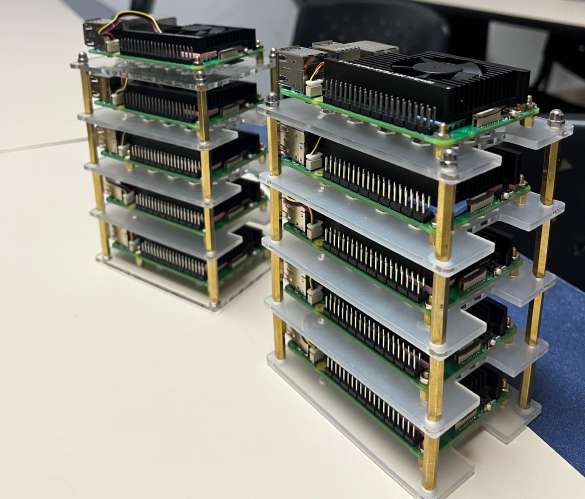
\includegraphics[width=0.6\textwidth]{figuras/cluster_rpi.png}
        \caption[Clúster de Raspberry Pi]{Clúster de Raspberry Pi. Fuente: Propia.}
        \label{fig:cluster}
    \end{figure}
    
    Un clúster de bajo consumo energético, como el de la Figura~\ref{fig:cluster}, es un sistema de cómputo distribuido conformado por múltiples nodos interconectados mediante una red de comunicación, cuyo diseño prioriza la eficiencia energética como criterio fundamental de construcción y operación. A diferencia de los sistemas HPC tradicionales, que priorizan el rendimiento computacional a expensas de un elevado consumo eléctrico, los clústeres de bajo consumo buscan maximizar la relación entre capacidad de procesamiento y energía consumida, expresada comúnmente en métricas como operaciones de punto flotante por vatio (FLOPS/W) o, en el contexto bioinformático, lecturas procesadas por unidad de energía (reads/Wh) \citep{pyrhonen2025energy}.
    
    \subsection{Raspberry Pi 5 y arquitectura ARM64}
    
    La Raspberry Pi 5, mostrada en la Figura~\ref{fig:rpi5}, llegó al mercado en 2023 como la quinta generación de la línea de computadores de placa única (\textit{Single Board Computer}, SBC) de Raspberry Pi. Cuenta con un procesador Broadcom BCM2712 de cuatro núcleos ARM Cortex-A76 de 64 bits (ARM64) a velocidades de hasta 2,4~GHz \citep{pyrhonen2025energy}. A nivel de memoria, soporta hasta 16~GB de RAM LPDDR4X y, en cuanto a conectividad, ofrece puertos USB~3.0, interfaz PCIe~2.0, salida dual de video 4K y red Gigabit Ethernet \citep{rpi2023brief}.
    
    \begin{figure}[H]
        \centering
        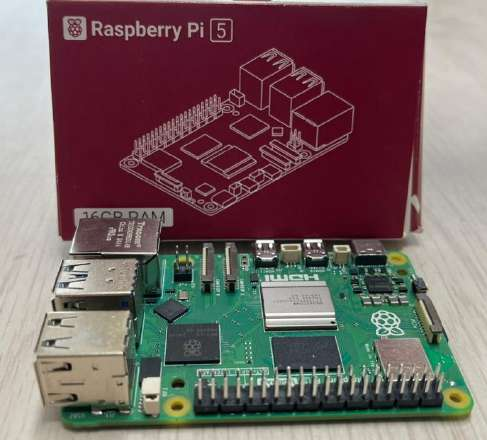
\includegraphics[width=0.55\textwidth]{figuras/raspberry_pi5.png}
        \caption[Tarjeta Raspberry Pi 5]{Visualización de la tarjeta Raspberry Pi 5. Fuente: Propia.}
        \label{fig:rpi5}
    \end{figure}
    
    La arquitectura ARM (\textit{Advanced RISC Machine}) de la RBPi5 se basa en el paradigma RISC (\textit{Reduced Instruction Set Computing}), caracterizado por un conjunto reducido de instrucciones que permite alcanzar un alto rendimiento por vatio consumido \citep{pyrhonen2025energy}. La arquitectura ARM64 introduce un conjunto ampliado de registros de propósito general y brinda soporte nativo para operaciones de punto flotante y extensiones SIMD (\textit{Single Instruction, Multiple Data}) a través del conjunto de instrucciones NEON, las cuales son importantes para acelerar operaciones de procesamiento de datos biológicos como el alineamiento de secuencias \citep{pyrhonen2025energy}. Gracias a esta configuración, un clúster basado en RBPi5 se presenta como una alternativa viable para desplegar los entornos bioinformáticos descritos anteriormente, siempre que estos sean adaptados a la arquitectura ARM64 y el análisis a un número limitado de muestras.
    
    %------------------------------------------------------------------------------
    
    \section{Estado del arte}
    
    \subsection{Clústeres con arquitectura ARM64}
    
    La evolución de los computadores de placa única ha permitido que superen el ámbito educativo, consolidándose como componentes viables y eficientes en infraestructuras de cómputo científico.
    
    Un caso destacado es el de \citet{abrahamsson2013}, quienes exploraron la viabilidad de nubes de bajo costo conectando 300 microcomputadores SBC en la Universidad Libre de Bolzano. Los investigadores mostraron que las limitaciones individuales de cada dispositivo pueden mitigarse mediante el paralelismo, de modo que el clúster, trabajando de forma simultánea, logra un rendimiento que supera las capacidades individuales de sus componentes.
    
    Otro ejemplo es el documentado por \citet{miller2017}, sobre el uso de 750 microcomputadores en el Laboratorio Nacional de Los Álamos para la creación de entornos de prueba a gran escala. Esta arquitectura resultó significativamente más eficiente desde el punto de vista energético que un supercomputador tradicional, manteniendo las capacidades necesarias para la validación y el desarrollo de software complejo.
    
    En cuanto al rendimiento en entornos científicos, \citet{maqbool2015arm} mostraron que la arquitectura ARM ofrece una escalabilidad superior a x86 en aplicaciones con alta demanda de entrada y salida (E/S), con resultados competitivos en ancho de banda y eficiencia energética. Asimismo, \citet{warade2022} validaron que el uso de clústeres de bajo consumo puede reducir el gasto energético total hasta en un 68\,\% mediante una gestión optimizada de recursos.
    
    Teniendo en cuenta estos antecedentes, la Raspberry Pi 5 introducida a finales de 2023 representa una evolución técnica relevante: gracias a su procesador Broadcom BCM2712 con cuatro núcleos ARM Cortex-A76 a 2.4~GHz e interfaz PCIe, amplía notablemente las capacidades de procesamiento de placas de bajo consumo frente a generaciones previas, permitiendo abordar la ejecución de pipelines bioinformáticos de análisis de amplicones en esquemas paralelos y distribuidos \citep{rpi2023brief}.
    
    \subsection{Pipelines de análisis de amplicones 16S en arquitecturas alternativas (GPU, FPGA, RISC-V)}
    
    El procesamiento de datos de 16S rRNA ha buscado históricamente la aceleración mediante hardware especializado para mitigar el cuello de botella que supone el volumen de lecturas. En arquitecturas basadas en unidades de procesamiento gráfico (GPU) se han desarrollado herramientas de clasificación taxonómica masiva que aprovechan el paralelismo de hilos para procesos de reducción de ruido y asignación de \textit{k}-mers. La aceleración por GPU ha permitido que herramientas como Kraken~2 alcancen velocidades de procesamiento órdenes de magnitud superiores a las de una CPU estándar, especialmente en metagenómica \textit{shotgun} y amplicones, aunque este incremento conlleva un consumo energético considerablemente mayor \citep{wood2019kraken2, robinson2021hardware}.
    
    Por otro lado, la industria ha adoptado arquitecturas basadas en matrices de puertas lógicas programables en campo (FPGA), que permiten acelerar el alineamiento de secuencias y el conteo de variantes directamente en hardware. A diferencia de las GPU, las FPGA logran reducir la latencia del pipeline con un menor consumo energético, ya que su diseño configurable permite adaptar los caminos de datos al algoritmo específico, evitando el desperdicio de energía en operaciones innecesarias \citep{robinson2021hardware}.
    
    Finalmente, la arquitectura de código abierto RISC-V \citep{gomezsanchez2023riscv} ha comenzado a explorarse como una alternativa de ultra bajo consumo para el análisis de secuencias. Proyectos de investigación en computación de alto rendimiento han evaluado el desempeño de algoritmos de alineamiento sobre núcleos RISC-V, mostrando que, aunque su ecosistema de software aún está madurando, su diseño modular es adecuado para tareas bioinformáticas que requieren personalización a nivel de instrucción para mejorar la eficiencia energética \citep{gomezsanchez2023riscv, pyrhonen2025energy}.
    
    A pesar de estos avances, el alto costo, el elevado consumo de energía y la complejidad de configuración dificultan el uso de estas arquitecturas en entornos con recursos limitados. Esto hace necesario explorar plataformas accesibles, de bajo consumo y fácil implementación, como el clúster RBPi5 propuesto en este trabajo.
    
    %==============================================================================
    % CAPÍTULO 2: METODOLOGÍA
    %==============================================================================
    
    \chapter{Metodología}
    \label{cap:metodologia}
    
    El desarrollo del proyecto se estructuró en cuatro fases: (1) diseño y construcción del clúster RBPi5, (2) portabilidad e instalación de los pipelines sobre arquitectura ARM64, (3) validación funcional mediante datos de referencia, y (4) evaluación comparativa de desempeño y eficiencia energética frente a una arquitectura x86. Cada fase se llevó a cabo bajo la metodología Six Sigma, concebida por Bill Smith en 1986 \citep{purdue2021sixsigma}, aplicando el ciclo DMAIC (\textit{Define, Measure, Analyze, Improve, Control}), cuyo esquema general se presenta en la Figura~\ref{fig:dmaic}.
    
    \begin{figure}[H]
        \centering
        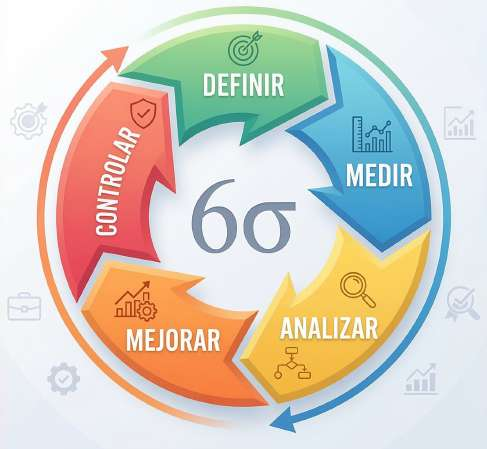
\includegraphics[width=0.5\textwidth]{figuras/six_sigma.png}
        \caption[Ciclo DMAIC de la metodología Six Sigma]{Ciclo DMAIC de la metodología Six Sigma. Fuente: generada con Gemini (versión 3).}
        \label{fig:dmaic}
    \end{figure}
    
    La metodología DMAIC fue concebida originalmente para la mejora de procesos existentes. En este proyecto, dado que el objeto de estudio es la construcción e implementación de un sistema tecnológico nuevo, sus etapas se adaptaron de la siguiente manera:
    
    \begin{itemize}
        \item \textbf{Definir:} establece los requerimientos y criterios de éxito de cada fase.
        
        \item \textbf{Medir:} caracteriza el estado inicial del sistema y documenta sus especificaciones técnicas.
        
        \item \textbf{Analizar:} examina los datos recopilados en la etapa anterior para identificar restricciones, incompatibilidades o cuellos de botella que orientan las decisiones técnicas.
        
        \item \textbf{Mejorar:} ejecuta las acciones correctivas o de implementación derivadas del análisis previo.
        
        \item \textbf{Controlar:} verifica la estabilidad y reproducibilidad del sistema antes de avanzar a la siguiente fase.
    \end{itemize}
    
    %------------------------------------------------------------------------------
    \section{Entornos experimentales}
    \label{sec:entornos}
    
    Para la evaluación comparativa se definieron tres entornos experimentales que permiten contrastar la arquitectura ARM64 frente a x86, así como evaluar el impacto de la virtualización ligera sobre x86 mediante la ejecución en Linux nativo y bajo WSL2, tal como se sintetiza en la Tabla~\ref{tab:entornos}.
    
    El primer entorno corresponde al clúster de bajo consumo (Green HPC), conformado por un nodo maestro Raspberry Pi 4 Model B (Broadcom BCM2711 de cuatro núcleos Cortex-A72 a 1.8~GHz y 8~GB de RAM), encargado de la orquestación y los servicios del sistema, y por los cinco nodos de cómputo Raspberry Pi 5 asignados al proyecto, de los diez disponibles sobre todo el clúster. Cada nodo de cómputo cuenta con un procesador Broadcom BCM2712 de cuatro núcleos ARM Cortex-A76 a 2.4~GHz (20 núcleos de cómputo en total), 16~GB de memoria RAM LPDDR4X-4267 (80~GB en total) y una tarjeta MicroSD local de 64~GB (Clase 10, UHS-I U3) para el arranque del sistema operativo. El clúster opera con Ubuntu Server 24.04 LTS en todos sus nodos, utiliza una topología de red en estrella sobre un conmutador Gigabit Ethernet (1000BASE-T) y comparte las bases de datos y los archivos FASTQ mediante un servidor NFSv4 alojado en el nodo maestro y montado en \texttt{/shared}. La distribución y el control de los trabajos paralelos se gestionan con Slurm Workload Manager (versión 23.11), y la telemetría energética se toma a 1.0~Hz directamente de los rieles de alimentación de cada placa mediante el PMIC Renesas DA9091. La Figura~\ref{fig:entornos} resume la topología del clúster y las características de los tres entornos de experimentación.

    \begin{figure}[H]
    \centering
    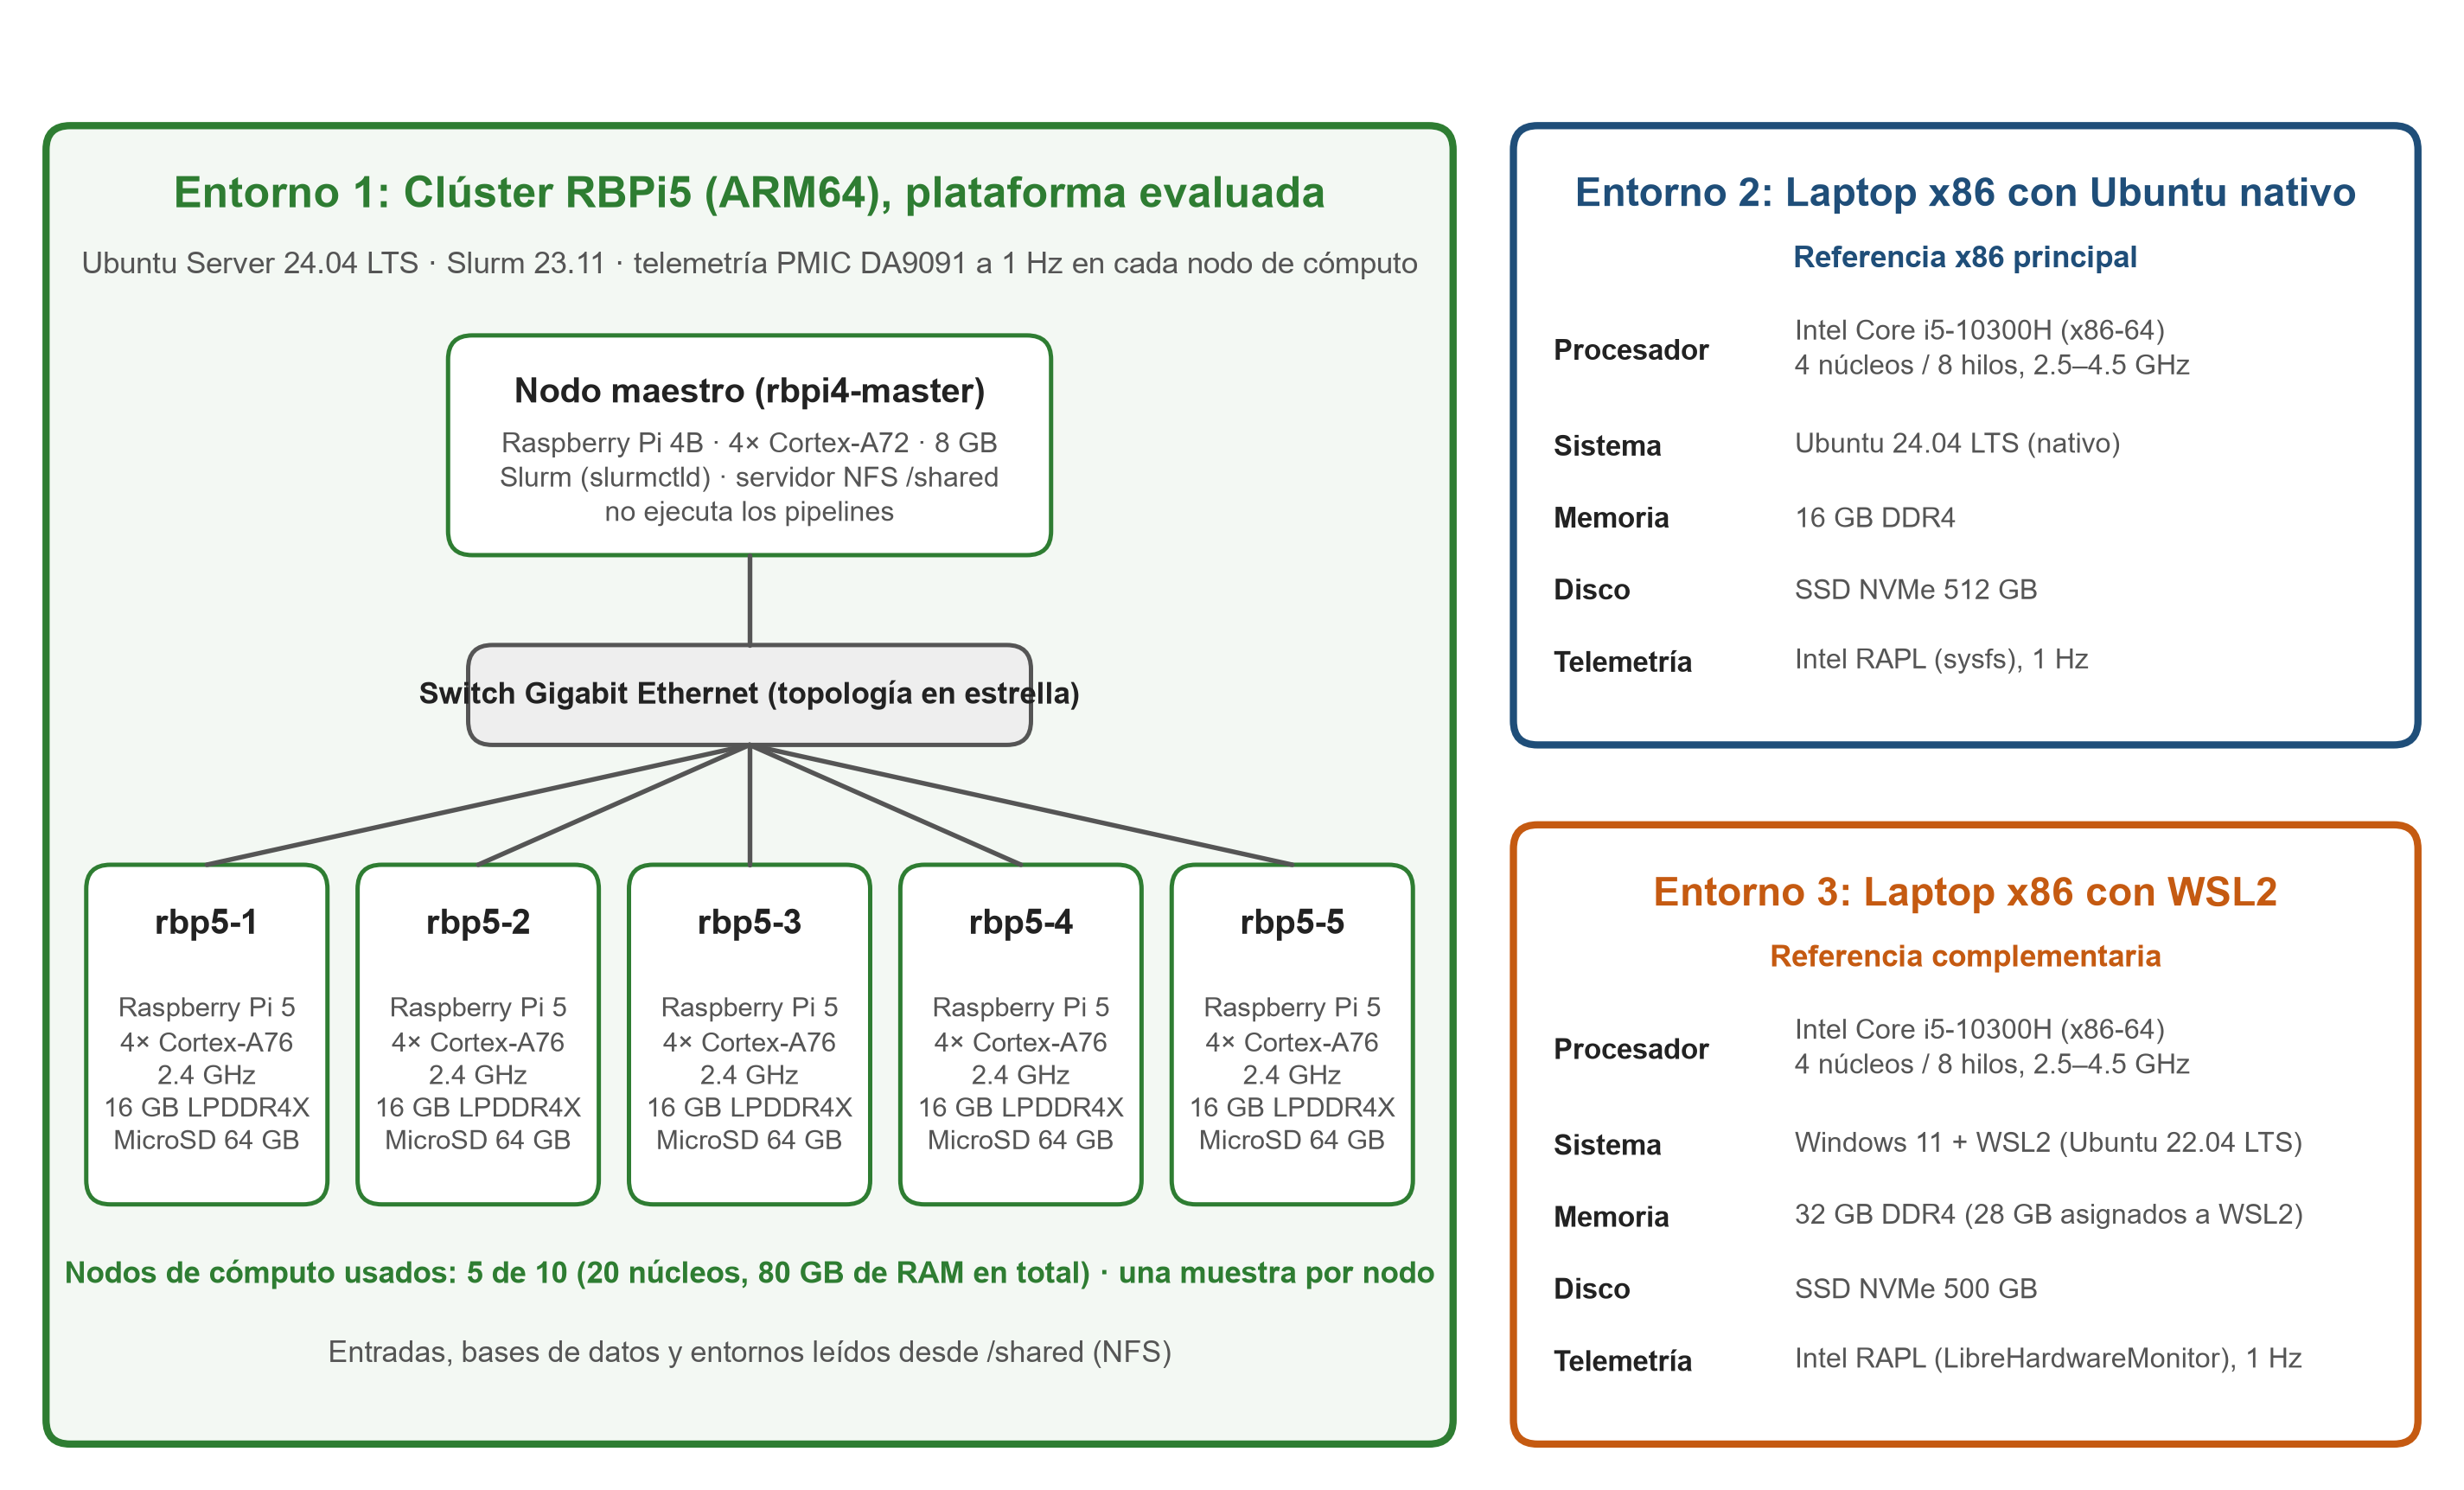
\includegraphics[width=\textwidth]{figuras/fig_entornos_experimentales.png}
    \caption{Entornos de experimentación: clúster RBPi5 con su topología de red, laptop x86 con Ubuntu nativo y laptop x86 con WSL2. Fuente: Propia.}
    \label{fig:entornos}
    \end{figure}
    
    El segundo entorno, utilizado como plataforma de referencia x86 principal, es un computador portátil con instalación nativa de Ubuntu 24.04 LTS (kernel Linux 6.8). Está equipado con un procesador Intel Core i5-10300H (4 núcleos físicos y 8 hilos lógicos a 2.50~GHz base, hasta 4.50~GHz turbo y 8~MB de caché), 16~GB de memoria RAM DDR4 a 2933~MHz en doble canal y una unidad de estado sólido SSD NVMe M.2 PCIe de 512~GB, lo que garantiza acceso directo al almacenamiento local sin sobrecargas de red. El consumo de potencia se registra a 1.0~Hz mediante la interfaz Intel RAPL en el dominio \texttt{package-0} a través de \texttt{sysfs}.
    
    El tercer entorno, empleado como referencia complementaria, evalúa la ejecución virtualizada sobre un computador portátil con sistema anfitrión Windows 11 ejecutando la distribución invitada Ubuntu 22.04 LTS dentro de WSL2. Desde la máquina virtual de WSL2 son visibles los 4 núcleos y 8 hilos del procesador Intel Core i5-10300H (2.50~GHz), y se le asignaron dinámicamente 28~GB de memoria RAM mediante el archivo de configuración \texttt{.wslconfig} (de los 32~GB de RAM DDR4 disponibles). A nivel de disco, WSL2 opera sobre una unidad virtual en formato VHDX montada sobre un SSD NVMe de 500~GB, con sistema de archivos ext4, donde se almacenaron los datos y las bases de referencia. Su telemetría energética se registró a 1.0~Hz capturando los contadores RAPL de la CPU mediante el servicio LibreHardwareMonitor en Windows.
    
    \begin{table}[H]
    \centering
    \caption{Plataformas de cómputo utilizadas en la evaluación.}
    \label{tab:entornos}
    \footnotesize
    \setlength{\tabcolsep}{4pt}
    \resizebox{\textwidth}{!}{%
    \begin{tabular}{l >{\raggedright\arraybackslash}p{4cm} >{\raggedright\arraybackslash}p{3.5cm} >{\raggedright\arraybackslash}p{3cm} >{\raggedright\arraybackslash}p{3cm} >{\raggedright\arraybackslash}p{3cm}}
    \toprule
    \textbf{Plataforma} & \textbf{Arquitectura (CPU)} & \textbf{RAM y Almacenamiento} & \textbf{Sistema operativo} & \textbf{Telemetría energética} & \textbf{Rol en el estudio} \\
    \midrule
    Clúster RBPi5 & ARM64 (20 núcleos Cortex-A76 @ 2.4~GHz) & 80~GB LPDDR4X (total), MicroSD 64~GB, NFS compartido & Ubuntu Server 24.04 LTS (Slurm 23.11) & PMIC DA9091 (hardware ADC) a 1.0~Hz & Plataforma evaluada (Green HPC)\\
    Computador x86 nativo & x86-64 (Intel Core i5-10300H) & 16~GB DDR4, SSD NVMe 512~GB & Ubuntu 24.04 LTS nativo & MSR/RAPL (\texttt{sysfs}) a 1.0~Hz & Referencia x86 principal \\
    Computador x86 WSL2 & x86-64 (Intel Core i5-10300H) & 32~GB DDR4 (28~GB para WSL2), SSD NVMe 500~GB & Ubuntu 22.04 LTS sobre WSL2 (Windows 11) & RAPL (LibreHardwareMonitor) a 1.0~Hz & Referencia complementaria \\
    \bottomrule
    \end{tabular}%
    }
    \end{table}
    
    La articulación de estos tres entornos permite desacoplar y evaluar dos factores fundamentales: el impacto de la microarquitectura de bajo consumo (ARM64 frente a x86) y la sobrecarga computacional inducida por la virtualización ligera (Linux nativo frente a WSL2). No obstante, es indispensable destacar una delimitación metodológica en la instrumentación: mientras que en el clúster Raspberry Pi~5 la telemetría del PMIC captura el consumo a nivel de placa completa, en las plataformas x86 la interfaz Intel RAPL registra exclusivamente el dominio del encapsulado (\texttt{package-0}). Esta asimetría física se consideró explícitamente en el protocolo de experimentación, orientando la evaluación tanto a la energía bruta como a la neta para garantizar una comparación rigurosa y transparente entre sistemas.

    
    
    
    
    %------------------------------------------------------------------------------
    \section{Fase 1: Diseño de la arquitectura hardware y software del clúster}
    \label{sec:fase1_metodologia}
    
    En esta fase se estructuró e implementó la arquitectura hardware y software del clúster de bajo consumo (Green HPC), compuesto por diez nodos de cómputo homogéneos Raspberry Pi 5 y un nodo maestro Raspberry Pi 4, definiendo la topología de red, el esquema de interconexión, la distribución de almacenamiento compartido y el sistema de telemetría energética para establecer la línea base de consumo del sistema en reposo (\textit{stand-by}) sobre arquitectura ARM64.
    
    \textbf{Definir.} Se formalizaron los requerimientos técnicos y funcionales del clúster para soportar cargas bioinformáticas altamente paralelas de procesamiento de secuencias masivas de amplicones 16S. A nivel de hardware, el clúster está organizado bajo un modelo maestro-trabajador y cuenta con un nodo maestro Raspberry Pi 4 Model B (\texttt{rbpi4-master}) y diez nodos de cómputo Raspberry Pi 5. Para este proyecto se utilizaron cinco de ellos (\texttt{rbp5-1} a \texttt{rbp5-5}), que suman 20 núcleos físicos ARM Cortex-A76 @ 2.4~GHz y 80~GB de memoria RAM LPDDR4X (16~GB por nodo de cómputo).
    
    A nivel de conectividad, se estableció una topología en estrella estructurada sobre un switch de red no administrado Gigabit Ethernet (1000BASE-T, IEEE 802.3ab) mediante cableado UTP Categoría 6, con un esquema de direccionamiento IPv4 estático privado dentro del segmento \texttt{192.168.1.100/24} a \texttt{192.168.1.105/24} y resolución local de nombres en \texttt{/etc/hosts}. El acceso al clúster se realizó de forma remota mediante SSH al nodo maestro, autenticándose con usuario y contraseña. Desde allí se enviaron los trabajos a los nodos de cómputo a través de Slurm (Versión 23.11.4). En cuanto a la infraestructura eléctrica, cada uno de los cinco nodos se dotó de una fuente de alimentación oficial Raspberry Pi USB-C de 27~W (5.1~V / 5.0~A con perfil Power Delivery), garantizando una entrega de corriente estable frente a picos transitorios de demanda de cómputo y evitando el estrangulamiento de frecuencia del microprocesador por subtensión (\textit{undervoltage throttling}). Finalmente, se definió el estado de reposo (\textit{stand-by}) como la condición operativa en la cual el nodo maestro y los cinco nodos de cómputo utilizados se encuentran completamente ensamblados, encendidos, conectados a la red local y con el kernel de Linux activo en modo multiusuario, pero sin procesos de análisis bioinformático en ejecución ni tráfico de datos en el bus de red.
    
    \textbf{Medir.} Para poder comparar el consumo de las plataformas, primero se levantó un inventario del hardware de cada equipo y se definió cómo se iba a medir la energía en cada una de ellas. 
    
    En la plataforma ARM64, la medición se tomó directamente de la placa mediante el circuito integrado de gestión de energía (PMIC, \textit{Power Management Integrated Circuit}) Renesas DA9091 disponible en cada Raspberry Pi 5. Este chip incluye un convertidor analógico-digital (ADC) de 12 canales que reporta el voltaje y la corriente de los rieles de alimentación de la placa. Estos valores se leyeron en cada nodo con la utilidad de firmware \texttt{vcgencmd pmic\_read\_adc}, llamada desde un script en Python de autoría propia (\texttt{medir\_energia\_pmic.py}) desarrollado específicamente para este proyecto, el cual captura los valores de los rieles a 1.0~Hz, calcula la potencia instantánea sumando el producto voltaje--corriente de todos los canales ($P = \sum V_i \cdot I_i$) y realiza la integración numérica para computar la energía consumida en vatios-hora.
    
    En las plataformas x86, la telemetría se fundamentó en la interfaz Intel RAPL (\textit{Running Average Power Limit}) para capturar el consumo del encapsulado del procesador en el dominio \texttt{package-0}, adaptando el mecanismo de recolección según el entorno del sistema operativo.
    
    En \textit{Ubuntu nativo} se empleó un script propio en Python (\texttt{medir\_energia\_rapl.py}) que consulta a 1.0~Hz los contadores de energía en microjulios expuestos por el kernel de Linux a través del pseudo-sistema de archivos \texttt{sysfs} (\texttt{/sys/}\allowbreak\texttt{class/}\allowbreak\texttt{powercap/}\allowbreak\texttt{intel-rapl:0/}\allowbreak\texttt{energy\_uj}).
    
    En \textit{WSL2 sobre Windows 11} dado que el hipervisor de virtualización de WSL2 no expone los registros MSR/RAPL en el sistema de archivos de la máquina invitada de Linux, la medición se realizó desde el sistema anfitrión Windows mediante un script automatizado en PowerShell acoplado al motor de telemetría de \textit{LibreHardwareMonitor}, registrando a 1.0~Hz el sensor de potencia del procesador (\textit{CPU Package Power}) de forma sincronizada con la ejecución del pipeline.
    
    Para obtener la línea base energética, en todas las plataformas se registró la potencia de cada equipo en reposo durante 5 minutos antes de cada corrida experimental tras un período de 60 segundos de estabilización previa sin medición, garantizando que únicamente los procesos fundamentales del sistema estuvieran en ejecución antes de iniciar el pipeline objetivo.
    
    
    
    
    
    \textbf{Analizar.} A partir de los requerimientos identificados y los mecanismos de medición formulados, se llevó a cabo un análisis de viabilidad técnica y condiciones operativas enfocado en cuatro factores críticos de diseño:

    En primer lugar, se analizó la capacidad de la infraestructura de comunicaciones frente a la demanda de datos bioinformáticos. Puesto que los pipelines requieren transferir concurrentemente conjuntos de lecturas FASTQ e índices taxonómicos desde el almacenamiento compartido NFS, se contrastó la tasa teórica del enlace Gigabit Ethernet (1000BASE-T, 125~MB/s) frente a los tamaños típicos de las muestras. Se determinó que una topología en estrella con resolución estática minimiza la latencia de conmutación y permite una distribución paralela eficiente, previendo que la lectura intensiva de bases de datos se beneficie de los búferes de memoria RAM local de cada nodo para descongestionar el tráfico de red.

    En segundo lugar, se examinó el balance de potencia eléctrica y estabilidad de voltaje. Las especificaciones del microprocesador Broadcom BCM2712 operando a 2.4~GHz proyectan consumos dinámicos elevados bajo estrés computacional sostenido. Por ello, el análisis de diseño determinó que el suministro eléctrico debía desacoplarse totalmente entre nodos mediante fuentes dedicadas de 27~W con perfil Power Delivery, mitigando riesgos de subtensión transitoria (\textit{undervoltage}) que pudieran degradar la frecuencia de reloj o reiniciar los nodos durante fases de cálculo intensivo.

    En tercer lugar, se evaluaron los márgenes de disipación térmica. Dado que el estrangulamiento térmico (\textit{thermal throttling}) en la Raspberry Pi~5 se activa automáticamente al alcanzar los $80^\circ$C reduciendo la frecuencia de la CPU, se estableció el criterio de que el sistema de enfriamiento activo por modulación de ancho de pulso (PWM) debía mantener la temperatura de los nodos con un margen de seguridad holgado respecto a dicho umbral crítico en todas las condiciones de reposo y operación.

Finalmente, se consideró analíticamente la asimetría de instrumentación entre plataformas: mientras que en el clúster ARM64 el sensor PMIC registra la potencia total disipada por la placa completa (procesador, memoria LPDDR4X y circuitería de soporte), la interfaz RAPL en x86 captura exclusivamente el dominio del encapsulado (\texttt{package-0}). Esta delimitación física fundamentó la necesidad analítica de formular dos métricas independientes de consumo (energía bruta y energía neta) para asegurar una evaluación comparativa transparente.

    
    
    \textbf{Mejorar.} Con el fin de mitigar posibles degradaciones de rendimiento y asegurar la máxima disponibilidad operativa, se llevaron a cabo optimizaciones tanto en el sistema operativo como en la pila de software de alto rendimiento:
    \newpage
    
    \begin{enumerate}
        \item \textit{Despliegue del gestor de colas Slurm:} Se instaló y configuró Slurm Workload Manager versión 23.11, desplegando el servicio central de control \texttt{slurmctld} en el nodo maestro y los servicios de ejecución \texttt{slurmd} en cada uno de los cinco nodos de cómputo, lo que permitió el despacho concurrente de tareas bioinformáticas.
        
        \item \textit{Aislamiento y control de recursos vía cgroups:} En entornos de memoria compartida (16~GB por nodo de cómputo), la ejecución concurrente de procesos científicos intensivos puede saturar la memoria física y activar el mecanismo \textit{OOM Killer} (\textit{Out-Of-Memory}) del kernel de Linux, congelando el nodo. Para prevenir esto, se integró el subsistema de grupos de control (\texttt{cgroups}) en el archivo de configuración \texttt{cgroup.conf} de Slurm, estableciendo techos máximos de memoria RAM por proceso (\texttt{AllowedRAMSpace=90\%}) y confinamiento estricto (\texttt{ConstrainRAMSpace=yes}), garantizando una reserva de memoria dedicada a las funciones críticas del sistema operativo y evitando desbordamientos de memoria.
        
        \item \textit{Almacenamiento distribuido compartido NFS:} Se implementó un servidor Network File System versión 4 (NFSv4) en el nodo maestro, exportando el directorio \texttt{/shared} hacia los cinco nodos de computo bajo las directivas de montaje \texttt{rw}, \texttt{sync}, \texttt{no\_root\_squash}, \texttt{no\_subtree\_check} con aceleración de lectura en búfer de memoria RAM local. Esta configuración unificó el acceso a los scripts, las bases de datos de referencia (GTDB y SILVA) y a los archivos FASTQ, evitando la redundancia de almacenamiento y eliminando la necesidad de duplicar decenas de gigabytes en las tarjetas MicroSD locales de cada trabajador.
        
        \item \textit{Configuración operativa del sistema operativo:} Cada nodo operó bajo Ubuntu Server 24.04 LTS en modalidad estrictamente sin interfaz gráfica (\textit{headless}, objetivo \texttt{multi-user.target}), verificándose la ausencia de servidores de video activos y la inactividad de las interfaces inalámbricas (Bluetooth y Wi-Fi), asegurando que el flujo de datos y la telemetría operaran exclusivamente sobre el controlador Gigabit Ethernet cableado para evitar consumos parásitos de radiofrecuencia.
    \end{enumerate}
    
    \textbf{Controlar.} Se establecieron protocolos automatizados de validación del estado y estabilidad del sistema. Mediante comandos nativos de Slurm (\texttt{sinfo}, \texttt{scontrol ping} y \texttt{squeue}) y scripts de prueba en Bash, se verificó la disponibilidad continua de los nodos de cómputo y la resolución bidireccional de red sin pérdidas de paquetes. Adicionalmente, se implementó un procedimiento de control de calidad para la telemetría energética: antes de autorizar las mediciones basales, se consultó el estado del PMIC en cada nodo mediante \texttt{vcgencmd pmic\_read\_adc}, validando la respuesta positiva y libre de anomalías en todos los canales de sensado ($P > 0$) tras el período de estabilización de 60 segundos, asegurando la consistencia e integridad de las lecturas eléctricas.

    
    %------------------------------------------------------------------------------
    \section{Fase 2: Portabilidad de los pipelines a ARM64}
    \label{sec:fase2_metodologia}
    
    En esta fase se abordó el reto de ingeniería de software consistente en portar, compilar y ejecutar de forma nativa en la arquitectura ARM64 (\texttt{aarch64}) tres pipelines bioinformáticos representativos para el análisis de amplicones 16S, asegurando su compatibilidad con el gestor de colas Slurm y optimizando su desempeño multihilo sobre el hardware del clúster.
    
    \textbf{Definir.} Como marco de referencia se tomó LEMMI16s \citep{seppey2025lemmi}, una plataforma para evaluar y comparar herramientas de clasificación taxonómica de amplicones 16S. LEMMI16s incluye los pipelines empaquetados en contenedores Docker o Singularity, lo que facilita su instalación y despliegue, y genera muestras sintéticas a partir de una composición taxonómica conocida, de modo que la clasificación obtenida por cada pipeline se puede comparar con la composición real (\textit{Ground Truth}). A partir de las herramientas disponibles en LEMMI16s se seleccionaron tres pipelines con enfoques algorítmicos distintos:
    
    \begin{enumerate}
        \item \textit{Kraken 2 (v2.1.3) + Bracken (v3.0.1):} Enfoque basado en alineamiento libre de k-mers (\textit{alignment-free}) y búsqueda exacta mediante minimizadores compactos indexados sobre la base de datos de referencia Genome Taxonomy Database (GTDB), seguido de una estimación de abundancias a nivel de especie mediante el algoritmo probabilístico de reestimación bayesiana de Bracken.
        
        \item \textit{LotuS3 Suite (v3.03):} Pipeline integral y ligero orientado al agrupamiento de secuencias en Unidades Taxonómicas Operacionales (OTUs). Integra el módulo de demultiplexación y filtrado de calidad estricto \texttt{sdm}, algoritmos de agrupamiento heurístico basados en identidad de secuencia (CD-HIT en el modo para lecturas largas PacBio) y asignación taxonómica mediante alineamiento con \texttt{vsearch} y el algoritmo del ancestro común más cercano (\textit{Lowest Common Ancestor}, LCA) contra la base de datos SILVA 138.1.
        
        \item \textit{QIIME 2 (q2cli 2022.8):} Entorno modular de referencia en microbiología computacional que genera Variantes de Secuencia de Amplicones (ASVs) mediante denoising estadístico por modelado de tasas de error de secuenciación (algoritmo Deblur) y clasificación taxonómica automatizada basada en clasificadores Naive Bayes entrenados sobre bases de referencia (\texttt{q2-feature-classifier}).    
    \end{enumerate}
    
    
    \textbf{Medir.} Se realizó una auditoría de dependencias binarias y librerías dinámicas requeridas por cada pipeline. Se identificaron los módulos nativos en C, C++, Fortran y Perl, así como la pila científica de Python (\texttt{numpy}, \texttt{scipy}, \texttt{scikit-learn}, \texttt{biopython}, \texttt{pandas}, \texttt{scikit-bio}, \texttt{h5py}). Para cada herramienta se evaluó la disponibilidad de paquetes precompilados para la arquitectura \texttt{aarch64} en canales comunitarios como Bioconda y Conda-Forge, identificando aquellas fuentes que exigían compilación manual desde el código fuente.
    
    \textbf{Analizar.} El análisis técnico de la portabilidad sobre la plataforma Raspberry Pi 5 evidenció tres obstáculos principales:
    
    \begin{enumerate}
        \item \textit{Restricción de contenedores Docker y Singularity/Apptainer:} Como se indicó al inicio de esta sección, LEMMI16s ejecuta sus pipelines dentro de contenedores Docker o Singularity/Apptainer. En el clúster, la construcción y ejecución de estos contenedores requería permisos de superusuario (\texttt{sudo}), los cuales no fueron otorgados a las cuentas del proyecto por la administración del clúster, dado que se trata de una infraestructura compartida en la que un cambio con privilegios de administrador podía afectar la configuración del sistema y el trabajo de otros usuarios. Adicionalmente, en Ubuntu Server 24.04 LTS el kernel aplica por omisión la directiva \texttt{kernel.}\allowbreak\texttt{apparmor\_}\allowbreak\texttt{restrict\_}\allowbreak\texttt{unprivileged\_}\allowbreak\texttt{userns = 1}, que impide la creación de espacios de nombres de usuario no privilegiados, por lo que la invocación de contenedores sin privilegios fallaba con errores de permisos (\texttt{EPERM}).
        
        \item \textit{Inviabilidad de la emulación dinámica con QEMU:} Aunque es posible ejecutar binarios x86\_64 en sistemas ARM64 mediante la capa de traducción QEMU User Emulation (\texttt{qemu-x86\_64-static}), este mecanismo introduce una penalización considerable en el tiempo de ejecución y altera las mediciones de potencia al agregar la sobrecarga de traducir instrucciones. Dado que el objetivo del trabajo es medir la eficiencia del procesador ARM64 frente a x86, la emulación fue descartada.
        
        \item \textit{Incompatibilidad de herramientas y versiones entre plataformas:} No todas las herramientas y versiones disponibles para x86\_64 contaban con soporte o paquetes precompilados para la arquitectura \texttt{aarch64}:
        
        En \textit{QIIME~2}, no existían metapaquetes recientes de distribución para ARM64, siendo \texttt{q2cli 2022.8} la única versión funcional y estable en el clúster, mientras que la plataforma x86 contaba con distribuciones más actualizadas.
        
        En \textit{Bracken}, el contenedor oficial de LEMMI16s en x86 empleaba la versión 2.8, pero los repositorios de Bioconda para \texttt{aarch64} únicamente disponían de la versión 3.0.1 (debido a la ausencia de compilaciones retrospectivas en la infraestructura ARM64 de Conda), lo que introducía divergencias en la estimación probabilística de abundancias.
        
        En \textit{LotuS3}, el alineador local predeterminado de la suite (\texttt{lambda3}) carece por completo de paquete o binario ejecutable para \texttt{aarch64}, forzando al clúster a recurrir a \texttt{vsearch}. Asimismo, componentes internos esenciales como el módulo de agrupamiento \texttt{usearch} y el clasificador \texttt{LCA} (\textit{Lowest Common Ancestor}) se distribuían únicamente como binarios precompilados para x86\_64, exigiendo compilación nativa desde código fuente en el clúster, mientras que ligeras discrepancias en la subversión de \texttt{vsearch} entre plataformas alteraban el número de lecturas asignadas en secuencias largas.
        
        Estas discrepancias de software y dependencias arquitectónicas impedían establecer una comparación experimental válida y reproducible si no se realizaba una homologación estricta previa.
    \end{enumerate}
    
    \textbf{Mejorar.} Para superar estos impedimentos se adoptaron las siguientes soluciones:
    
    \begin{enumerate}
        \item \textit{Transición a ejecución nativa en espacio de usuario:} Se desacoplaron los pipelines de la capa de contenedores y se instalaron de forma nativa, sin requerir permisos de superusuario, mediante entornos de Conda para la arquitectura \texttt{aarch64} alojados en el almacenamiento compartido: \texttt{lemmi16s\_env} (Kraken~2 + Bracken), \texttt{lemmi16s\_pacbio\_env} (LotuS3) y \texttt{qiime2\_arm64} (QIIME~2). Kraken~2, Bracken y los componentes \texttt{sdm} y \texttt{vsearch} se instalaron como paquetes precompilados para ARM64 desde Bioconda. LotuS3 se instaló a partir del paquete de Bioconda descargado manualmente, ya que la resolución automática de dependencias fallaba en ARM64. El módulo de agrupamiento \texttt{usearch12} se compiló desde su código fuente oficial para \texttt{aarch64}, y QIIME~2 (q2cli 2022.8) se instaló mediante \texttt{pip} sobre un entorno Python 3.8 de Conda-Forge.
    
        \item \textit{Alineación de versiones entre plataformas:} Durante la fase exploratoria preliminar se identificaron discrepancias entre los paquetes disponibles en los repositorios de cada plataforma (por ejemplo, Bracken 2.8 en x86 frente a 3.0.1 en ARM64). Para asegurar que las comparaciones experimentales reflejaran las características de la microarquitectura y no discrepancias de software, para todas las corridas finales comparativas de rendimiento, telemetría y fidelidad taxonómica se homologaron estrictamente las versiones en ambas plataformas: Kraken~2.1.3, Bracken 3.0.1, LotuS~3.03 y QIIME~2 (q2cli 2022.8). En la plataforma x86, Bracken se reinstaló de forma nativa a partir del repositorio oficial para igualar la versión 3.0.1 del clúster, y el entorno de QIIME~2 se ajustó a q2cli 2022.8. En LotuS3 se fijó además el alineador de la asignación taxonómica: Dado que LAMBDA3 no tiene paquete para \texttt{aarch64}, el clúster cambia automáticamente a \texttt{vsearch}. Para que las tres plataformas ejecutaran el mismo flujo, LotuS3 se corrió en todos los equipos con \texttt{vsearch} v2.31.0 (opción \texttt{-taxAligner vsearch}). Todas las tablas, figuras y resultados definitivos del presente trabajo corresponden exclusivamente a estas versiones homologadas.
    
    
        \item \textit{Orquestación distribuida vía scripts Slurm:} Se diseñaron scripts de sumisión por lotes que asignan cada muestra biológica de forma exclusiva a un nodo de cómputo (\texttt{--nodes=1 --exclusive}), operando sobre el almacenamiento compartido \texttt{/shared}. Para maximizar el aprovechamiento de los 4 núcleos Cortex-A76 sin saturar los buses de datos, Kraken~2 y LotuS3 se parametrizaron con 4 hilos por tarea, mientras que QIIME~2 se configuró con 2 hilos por tarea (\texttt{--cpus-per-task}) y un techo de contención de 14~GB (\texttt{--mem=14G}). Asimismo, como delimitación metodológica orientada a desacoplar el efecto de la aceleración distribuida frente a la eficiencia propia de la microarquitectura, se incorporó una condición experimental de control consistente en evaluar cada pipeline bajo ejecución secuencial (en un nodo físico de control) bajo las mismas restricciones operativas.
    
        \item \textit{Optimización de memoria y reducción del clasificador en QIIME~2:} El clasificador Naive Bayes (\texttt{q2-feature-classifier classify-sklearn}) entrenado sobre la base de datos taxonómica completa de SILVA (más de 500,000 secuencias no acotadas) demanda entre 32 y 64~GB de memoria RAM durante la clasificación, lo que provocaría el colapso inmediato por falta de memoria física (\textit{Out-of-Memory}, OOM) tanto en los nodos de la Raspberry Pi 5 (con 16~GB de RAM física compartida) como en las computadoras portátiles. Para mitigar esta restricción, como adaptación metodológica, se implementó el procedimiento de reducción y acotamiento sobre la base SILVA 138.1, extrayendo un conjunto curado de aproximadamente 62,000 secuencias representativas focalizadas en las regiones hipervariables V1--V2 (\texttt{referenceClassificator.qza}, 118~MB). Esta optimización acotó la huella máxima estimada de memoria a menos de 3~GB por proceso, permitiendo una ejecución fluida con 2 hilos por nodo sin riesgo de estrangulamiento de memoria ni degradación por contención de recursos.
    \end{enumerate}
    
    \textbf{Controlar.} Antes de iniciar las campañas de medición se verificó el funcionamiento de cada entorno nativo en el clúster y en las plataformas x86: se validó la homologación de versiones de cada herramienta (\texttt{kraken2 --version}, \texttt{bracken -v}, \texttt{lotus3 -v} y \texttt{qiime --version}) y se ejecutó una corrida de prueba piloto con una muestra biológica por pipeline para certificar la ausencia de fallos de segmentación. Adicionalmente, las secuencias FASTQ de entrada y el modelo clasificador entrenado (\texttt{referenceClassificator.qza}) fueron distribuidos de manera centralizada hacia el almacenamiento compartido NFS y las estaciones x86, validando su integridad criptográfica mediante sumas de verificación MD5 para asegurar que todas las plataformas procesaran exactamente las mismas entradas.
    
    %------------------------------------------------------------------------------
    \section{Fase 3: Validación de la integridad funcional}
    \label{sec:fase3_metodologia}
    
    En esta fase se validó la integridad funcional y la fidelidad biológica de los pipelines bioinformáticos ejecutados sobre la arquitectura ARM64, comparando de manera sistemática sus salidas frente a los resultados obtenidos en las estaciones de control x86 y contrastándolos contra conjuntos de datos de referencia con verdad de terreno conocida (\textit{Ground Truth}).
    
    \textbf{Definir.} Para asegurar una evaluación imparcial, rigurosa y estandarizada, se establecieron tres conjuntos de datos sintéticos de amplicones 16S con una composición definida, generados por la plataforma de referencia internacional LEMMI16s \citep{seppey2025lemmi}, los cuales fueron:
    
    \begin{enumerate}
        \item \textit{Dataset HOMD\_v4\_GTDB (Kraken 2 + Bracken):} Comunidad sintética representativa del microbioma oral humano generada a partir de secuencias del gen 16S rRNA de longitud completa, de las cuales se simularon lecturas pareadas de 200~pb con el perfil Illumina MiSeq v3. Comprende 2,453,431 lecturas pareadas distribuidas en 5 muestras independientes (\texttt{c001}, \texttt{c002}, \texttt{c003}, \texttt{e001} y \texttt{e002}), analizadas contra el índice taxonómico de GTDB.
    
        \item \textit{Dataset HM\_Contaminated\_Soil (LotuS3 Suite):} Comunidad simulada de suelo contaminado con metales pesados, con lecturas PacBio HiFi del gen 16S rRNA completo generadas por la versión de LEMMI16s para lecturas largas (herramienta MHASS, perfil PacBio Sequel). Comprende 25,611 lecturas de una sola hebra, con una longitud media de 1,505~pb, en 5 muestras: tres de calibración (\texttt{c001}, \texttt{c002} y \texttt{c003}), que se usan para elegir el umbral de filtrado que maximiza el F1, y dos de evaluación (\texttt{e001} y \texttt{e002}), con las que se mide el desempeño final. Las muestras se generaron una sola vez y se copiaron a las tres plataformas, verificando con sumas MD5 que fueran idénticas.
        
        \item \textit{Dataset alfa\_v1v2\_SILVA (QIIME 2):} Amplicones correspondientes a las regiones hipervariables V1--V2 del gen 16S rRNA secuenciados mediante tecnología Illumina, abarcando un total de 2,690,077 lecturas pareadas en 5 muestras biológicas (\texttt{c001}, \texttt{c002}, \texttt{c003}, \texttt{e001} y \texttt{e002}), evaluadas mediante el clasificador Naive Bayes entrenado sobre SILVA 138.  
    \end{enumerate}
    
    \textbf{Medir.} Se ejecutaron los tres pipelines utilizando idénticos archivos FASTQ de entrada, versiones de bases de datos y parámetros de filtrado tanto en la estación de trabajo x86 nativa como en el clúster RBPi5. Las salidas computacionales (tablas de características, perfiles de abundancia relativa y asignaciones taxonómicas) se transformaron a matrices tabulares unificadas. Se definieron formalmente las métricas estadísticas para cuantificar la fidelidad biológica de cada pipeline frente al archivo oficial del Ground Truth (\texttt{queryTaxo.tsv}):
    
    \begin{itemize}
        \item \textit{Verdaderos Positivos ($TP$):} Número de taxones (familias, géneros o especies) identificados por el pipeline que coinciden biológica y taxonómicamente con los taxones presentes en el \textit{Ground Truth}.
        
        \item \textit{Falsos Positivos ($FP$):} Número de taxones predichos por el pipeline que no están presentes en la verdad de terreno (asignaciones espurias o ruido metagenómico).
        
        \item \textit{Falsos Negativos ($FN$):} Número de taxones presentes en el \textit{Ground Truth} que el pipeline no logró detectar (omisiones taxonómicas).
        
        \item \textit{Taxones de Verdad de Terreno ($GT$):} Número total de linajes biológicos verdaderos contenidos en la muestra simulada ($GT = TP + FN$).
    \end{itemize}
    
    A partir de estas variables se calcularon la Precisión ($P$), la Sensibilidad (\textit{Recall}, $R$) y la media armónica o puntuación F1 (\textit{F1-Score}, $F_1$) para cada muestra y nivel taxonómico:
    \begin{equation}
        P = \frac{TP}{TP + FP}, \qquad R = \frac{TP}{TP + FN}, \qquad F_1 = 2 \cdot \frac{P \cdot R}{P + R} = \frac{2 \cdot TP}{2 \cdot TP + FP + FN}
        \label{eq:metricas_biologicas}
    \end{equation}
    
    Adicionalmente, para verificar la reproducibilidad cruzada entre plataformas (x86 frente a ARM64), se calculó la concordancia taxonómica absoluta mediante la comparación diferencial de archivos línea por línea (\texttt{diff -u}), la verificación de coincidencia en los linajes taxonómicos detectados y la comparación de los perfiles de abundancia relativa.
    
    \textbf{Analizar.} El análisis de la integridad biológica se estructuró a partir de dos niveles complementarios de evaluación entre las salidas generadas en la arquitectura ARM64 y las estaciones de control x86:
    
    En primer lugar, se estableció un análisis computacional orientado a verificar el determinismo algorítmico entre plataformas mediante la inspección diferencial directa (\texttt{diff -u}) de los archivos de predicción taxonómica y perfiles de abundancia. Este análisis permitió evaluar si las diferencias arquitectónicas en los conjuntos de instrucciones o en las unidades de coma flotante introducían variaciones en los métodos deterministas (como la concordancia de k-mers en Kraken~2 o el modelado de Deblur en QIIME~2).
    
    En segundo lugar, se formuló un análisis de consistencia biológica enfocado en comparar la robustez taxonómica frente a la verdad de terreno. Dado que flujos como LotuS3 incorporan etapas de agrupamiento heurístico y alineamiento local en secuencias de longitud completa (PacBio HiFi), el análisis se centró en corroborar si posibles variaciones menores en la agregación estocástica de lecturas alteraban la identificación de linajes clave o si, por el contrario, los perfiles taxonómicos a nivel de familia y género se mantenían biológicamente equivalentes en todas las plataformas.
    
    Con base en estos dos ejes, se definieron los criterios de aceptación analítica: para validar la reproducibilidad entre arquitecturas se requirió la preservación de los taxones biológicos verdaderos y la invariabilidad de las métricas de clasificación ($P$, $R$ y $F_1$), asegurando que cualquier cambio de plataforma no introdujera sesgos metodológicos ni divergencias en la interpretación biológica de las comunidades microbianas.
    
    
    \textbf{Mejorar.} Se ajustaron los parámetros de umbral de filtrado de calidad y longitud mínima de lecturas en los scripts de ejecución para garantizar que ningún pipeline descartara fragmentos válidos de secuencias por diferencias en la interpretación de caracteres ASCII. Asimismo, se unificaron las versiones de los índices de referencia en el volumen NFS para evitar discrepancias temporales en la resolución de linajes taxonómicos.
    
    \textbf{Controlar.} Las tablas de taxonomía resultantes de cada corrida se evaluaron con el procedimiento de análisis del benchmark LEMMI16s, que compara las predicciones frente al archivo de referencia \texttt{queryTaxo.tsv} para obtener las métricas de la Ecuación~\eqref{eq:metricas_biologicas}. Al revisar ese procedimiento se encontró que el evaluador de LEMMI16s calcula todas las muestras de evaluación con la verdad de terreno de la primera de ellas (\texttt{input.truth[0]} en el archivo \texttt{eval.smk}), por lo que el F1 se recalculó con la misma lógica de LEMMI16s (umbral de calibración y normalización por número de copias del gen), pero usando para cada muestra su propio archivo \texttt{queryTaxo.tsv}. Adicionalmente, las predicciones del clúster se compararon directamente con las obtenidas en x86 mediante \texttt{diff -u}, verificando que las diferencias entre plataformas fueran nulas o se limitaran a variaciones menores en los conteos.
    
    %------------------------------------------------------------------------------
    \section{Fase 4: Evaluación de desempeño y eficiencia energética}
    \label{sec:fase4_metodologia}
    
    En esta fase se evaluó experimentalmente el desempeño computacional, el consumo eléctrico y la eficiencia energética de las tres plataformas de cómputo bajo estudio, estableciendo un protocolo estandarizado de medición para formular la relación de eficiencia en lecturas procesadas por vatio-hora (\textit{Reads/Wh}).
    
    \textbf{Definir.} Se definió un protocolo de medición común para las tres plataformas, con el fin de que cada corrida comenzara con el equipo sin carga y sin actividad previa que alterara la potencia medida. Cada sesión experimental se estructuró en tres fases continuas:
\newpage

    \begin{enumerate}
        \item \textit{Estabilización (60 segundos, sin medición):} Tras lanzar el script de medición, el sistema permanece sin carga para que terminen los procesos residuales del arranque y la actividad previa.
        \item \textit{Línea base previa en reposo (Pre-run idle, 5 minutos):} El sistema se mantiene sin carga de procesamiento y se registra la potencia a 1.0~Hz. Su promedio es la potencia basal $\bar{P}_{\text{idle}}$ de esa sesión.
        \item \textit{Fase de cómputo activo (Active computation):} Se ejecuta el pipeline bioinformático completo bajo orquestación de Slurm en el clúster o mediante ejecución nativa en las estaciones x86, registrando de manera continua a 1.0~Hz la potencia instantánea disipada $P(\tau)$.
    \end{enumerate}
    
    La estandarización de este protocolo responde a la necesidad de controlar la deriva térmica residual: ensayos preliminares de calibración indicaron que intervalos de reposo breves (inferiores a un minuto) son susceptibles a sobrestimaciones de la potencia basal debido al calor acumulado y a procesos residuales del sistema operativo inmediatamente posteriores a una tarea previa. Por esta razón, se adoptó formalmente un intervalo de estabilización pasiva de 60~segundos seguido de 300~segundos (5~minutos) de registro continuo, garantizando una estimación robusta y asintóticamente estable de $\bar{P}_{\text{idle}}$ para cada sesión experimental.
    
    Además, para separar el efecto del paralelismo, cada pipeline se evaluó bajo un esquema de ejecución secuencial en el clúster (QIIME~2 y LotuS3 en \texttt{rbp5-1}, \texttt{rbp5-2}, y Kraken~2 en \texttt{rbp5-3}), procesando todas sus muestras una tras otra con el mismo protocolo, los mismos hilos por tarea y las mismas entradas que en la ejecución distribuida, lanzado mediante Slurm con acceso exclusivo al nodo.
    
    \textbf{Medir.} A lo largo de la ejecución de cada pipeline se adquirieron concurrentemente las siguientes variables físicas y computacionales:
    \begin{itemize}
        \item \textit{Tiempo de ejecución ($t$):} Duración en segundos de la ventana de medición de la fase activa, desde la primera hasta la última lectura de potencia. Es el mismo intervalo sobre el que se integra la energía. En el clúster corresponde a la ventana conjunta de los nodos, desde el primero que inicia hasta el último que termina.
        \item \textit{Carga de CPU ($\%$):} Porcentaje promedio de utilización de los núcleos de procesamiento muestreado a través del subsistema \texttt{procfs} de Linux (\texttt{/proc/stat}) y reportado a nivel de sistema.
        \item \textit{Memoria RAM máxima (\text{GB}):} Huella máxima de memoria física residente (\textit{Resident Set Size}, RSS) ocupada por los procesos bioinformáticos a lo largo del flujo.
        \item \textit{Potencia media en carga ($\bar{P}_{\text{activa}}$):} Promedio temporal de la potencia eléctrica total disipada durante la fase activa, expresada en vatios (W).
        \item \textit{Potencia media en reposo ($\bar{P}_{\text{idle}}$):} Potencia eléctrica basal registrada durante el intervalo previo de reposo, correspondiente al costo energético de mantener la plataforma encendida y operativa.
    \end{itemize}
    
    \textbf{Analizar.} Para analizar de forma física y matemáticamente rigurosa el gasto energético, se formuló el balance eléctrico del sistema. La potencia neta atribuible exclusivamente al cálculo computacional ($P_{\text{neta}}$) se calculó sustrayendo el consumo basal en reposo de la potencia activa:
    \begin{equation}
        P_{\text{neta}}(\tau) = P_{\text{activa}}(\tau) - \bar{P}_{\text{idle}} \qquad [\text{W}]
        \label{eq:potencia_neta}
    \end{equation}
    
    A partir de la potencia instantánea se calculó la energía total consumida ($E_{\text{total}}$) y la energía neta computacional ($E_{\text{neta}}$), integradas en el dominio temporal y expresadas en vatios-hora (Wh). Como la potencia se registra en lecturas discretas $P_i$ tomadas en los instantes $t_i$ ($i = 1, \dots, n$), la integral se evaluó numéricamente mediante la regla del trapecio sobre las marcas de tiempo reales de cada lectura:
    
    \begin{equation}
        E_{\text{total}} = \frac{1}{3600}\int_{t_1}^{t_n} P_{\text{activa}}(\tau)\,d\tau \approx \frac{1}{3600}\sum_{i=1}^{n-1} \frac{P_{i} + P_{i+1}}{2}\,(t_{i+1} - t_{i}) \qquad [\text{Wh}]
        \label{eq:energia_total}
    \end{equation}
    \begin{equation}
        E_{\text{neta}} = \frac{1}{3600}\int_{t_1}^{t_n} P_{\text{neta}}(\tau)\,d\tau \approx \frac{1}{3600}\sum_{i=1}^{n-1} \left(\frac{P_{i} + P_{i+1}}{2} - \bar{P}_{\text{idle}}\right)(t_{i+1} - t_{i}) \qquad [\text{Wh}]
        \label{eq:energia_neta}
    \end{equation}
    
    La evaluación numérica mediante la regla del trapecio sobre marcas de tiempo reales $(t_{i+1} - t_{i})$, en lugar de asumir un paso de discretización constante, se fundamenta en el comportamiento temporal del sistema operativo: bajo cargas computacionales intensivas, la contención en la planificación de procesos en espacio de usuario puede introducir pequeñas fluctuaciones en la frecuencia efectiva de muestreo de la telemetría. La integración temporal sobre intervalos reales garantiza la exactitud del cómputo energético acumulado. En el clúster, la energía se calculó de forma independiente para cada nodo de cómputo empleando su respectivo $\bar{P}_{\text{idle}}$, computando posteriormente el consumo agregado del sistema.
\newpage

    La energía total ($E_{\text{total}}$) es toda la energía que consumió el equipo durante la corrida, incluida la que gasta solo por estar encendido. La energía neta ($E_{\text{neta}}$) es la energía total menos la que el equipo habría consumido en reposo durante el mismo tiempo ($\bar{P}_{\text{idle}} \cdot t$), es decir, la energía adicional que exigió el pipeline. La energía total refleja lo que realmente se paga en electricidad, mientras que la energía neta permite comparar cuánto consume el cómputo en sí, sin el efecto del consumo en reposo de cada plataforma.
    
    Para cuantificar el rendimiento biológico por unidad de energía eléctrica consumida, se formuló la métrica principal de eficiencia energética ($\eta$), definida como el número total de lecturas biológicas procesadas ($N_{\text{reads}}$) por cada vatio-hora invertido:
    \begin{equation}
        \eta_{\text{bruta}} = \frac{N_{\text{reads}}}{E_{\text{total}}} \quad \left[\frac{\text{reads}}{\text{Wh}}\right], \qquad \eta_{\text{neta}} = \frac{N_{\text{reads}}}{E_{\text{neta}}} \quad \left[\frac{\text{reads}}{\text{Wh}}\right]
        \label{eq:eficiencia}
    \end{equation}
    
    Finalmente, para cuantificar la ventaja relativa de una plataforma sobre otra, se definió el factor de ganancia verde o aceleración energética relativa ($G_{\text{verde}}$) como la razón entre la eficiencia alcanzada por el clúster ARM64 frente a la estación x86:
    \begin{equation}
        G_{\text{verde}} = \frac{\eta_{\text{clúster}}}{\eta_{\text{x86}}}
        \label{eq:ganancia_verde}
    \end{equation}
    
    \textbf{Mejorar.} Con el fin de aislar estrictamente el costo energético del procesamiento biológico y evitar sobreestimaciones por etapas accesorias, se estableció como directriz metodológica la preindexación de las bases de datos de referencia: tanto el índice de \texttt{vsearch} para LotuS3 (archivo en formato UDB de aproximadamente 3~GB) como los índices taxonómicos de Kraken~2 se generaron de forma centralizada previo a las sesiones de prueba. De este modo, la ventana de telemetría capturó de manera pura el consumo derivado del control de calidad, agrupamiento, inferencia y clasificación taxonómica de las muestras, eliminando el sesgo de las fases de preparación de datos.
    
    \textbf{Controlar.} Para asegurar la validez y comparabilidad de las mediciones, cada corrida experimental se normalizó exclusivamente frente al reposo basal ($\bar{P}_{\text{idle}}$) registrado en su propia sesión y entorno térmico. Asimismo, se estableció un protocolo de verificación de estabilidad que descartó cualquier sesión experimental que presentara derivas basales o anomalías en la telemetría al finalizar el procesamiento, garantizando que las integrales de energía neta calculadas reflejaran de forma fidedigna el esfuerzo computacional de los pipelines bioinformáticos.
    
    
    
    %==============================================================================
    % CAPÍTULO 3: RESULTADOS
    %==============================================================================
    
    \chapter{Resultados}
    \label{cap:resultados}
    
    En este capítulo se presentan los resultados obtenidos en cada una de las fases del proyecto. En todos los casos, la comparación principal se realiza entre el clúster RBPi5 y el computador x86 con Ubuntu nativo. Los resultados obtenidos en WSL2 se incluyen como referencia complementaria.
    
    %------------------------------------------------------------------------------
    \section{Fase 1: Clúster RBPi5 y línea base energética}
    
    El clúster quedó conformado como se describió en la Sección~\ref{sec:fase1_metodologia} y se muestra en la Figura~\ref{fig:cluster_montado}: un nodo maestro Raspberry Pi~4B, que solo coordina las tareas mediante Slurm y comparte el directorio \texttt{/shared} por NFS, y diez nodos de cómputo Raspberry Pi~5 conectados por un switch Gigabit Ethernet, de los cuales cinco fueron asignados al proyecto (\texttt{rbp5-1} a \texttt{rbp5-5}). Antes de cada corrida se verificó con \texttt{sinfo} que los cinco nodos de cómputo estuvieran disponibles en estado \texttt{idle} (Figura~\ref{fig:sinfo_cluster}). La Tabla~\ref{tab:standby} presenta la potencia en reposo de cada nodo de cómputo, medida con el PMIC de la placa durante los 5 minutos previos a cada corrida.
    
    
    \begin{figure}[H]
    \centering
    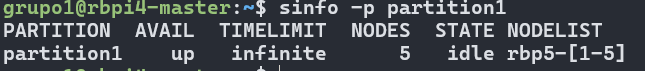
\includegraphics[width=0.7\textwidth]{figuras/sinfo_cluster.png}
    \caption{Estado de los cinco nodos de cómputo en la partición \texttt{partition1} de Slurm. Fuente: Propia.}
    \label{fig:sinfo_cluster}
    \end{figure}
    
    \begin{figure}[H]
    \centering
    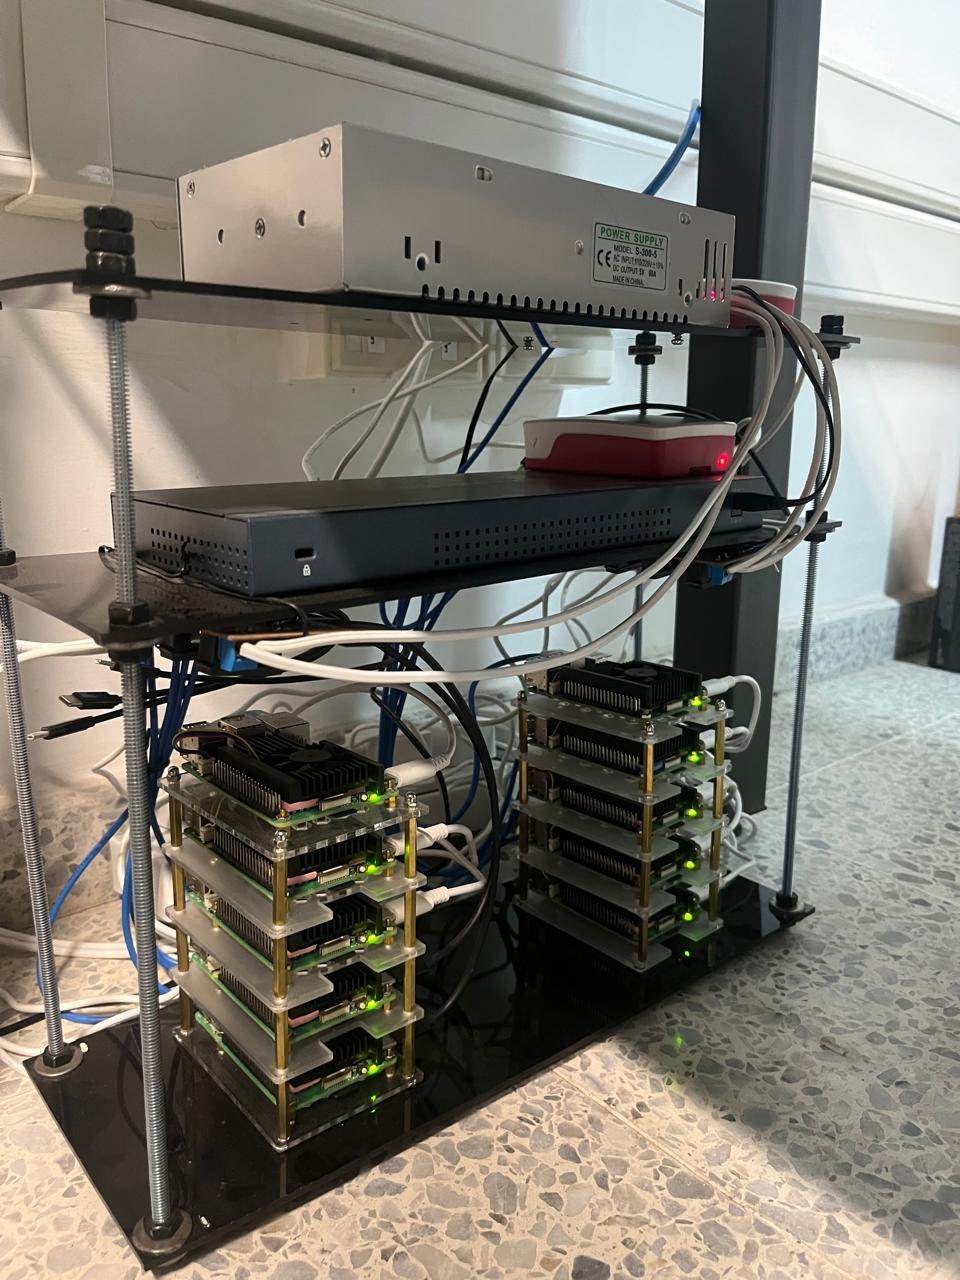
\includegraphics[width=0.6\textwidth]{figuras/cluster_montado.jpg}
    \caption{Clúster RBPi5 en operación: nodo maestro Raspberry Pi~4B (caja roja), switch Gigabit Ethernet y dos torres de cinco nodos de cómputo Raspberry Pi~5. Fuente: Propia.}
    \label{fig:cluster_montado}
    \end{figure}
    
    \begin{table}[H]
    \centering
    \caption{Potencia en reposo (\textit{stand-by}) de los nodos de cómputo del clúster RBPi5, promedio de las mediciones de 5 minutos previas a cada corrida.}
    \label{tab:standby}
    \small
    \begin{tabular}{l c}
    \toprule
    \textbf{Nodo de cómputo} & \textbf{Potencia en reposo (W)} \\
    \midrule
    \texttt{rbp5-1} & 2.389 \\
    \texttt{rbp5-2} & 2.377 \\
    \texttt{rbp5-3} & 2.420 \\
    \texttt{rbp5-4} & 2.379 \\
    \texttt{rbp5-5} & 2.332 \\
    \midrule
    \textbf{Total (5 nodos de cómputo)} & \textbf{11.896} \\
    \bottomrule
    \end{tabular}
    \end{table}
    
    
    El nodo maestro (Raspberry Pi 4B) no se incluye en esta caracterización, ya que no incorpora el PMIC DA9091 y no participa en la ejecución de los pipelines. Su función se limita a la coordinación de tareas mediante Slurm y al servicio de almacenamiento compartido NFS.
    
    %------------------------------------------------------------------------------
    \section{Fase 2: Pipelines portados a ARM64}
    Se lograron portar, compilar y ejecutar con éxito los tres pipelines de análisis de amplicones 16S sobre la arquitectura ARM64 con Ubuntu Server 24.04 LTS. La Tabla~\ref{tab:pipelines} detalla las herramientas adaptadas, sus versiones y los ajustes técnicos requeridos.
    
    \begin{table}[H]
    \centering
    \caption{Pipelines portados a la arquitectura ARM64.}
    \label{tab:pipelines}
    \footnotesize
    \setlength{\tabcolsep}{4.5pt}
    \resizebox{\textwidth}{!}{%
    \begin{tabular}{>{\raggedright\arraybackslash}p{2.8cm} >{\raggedright\arraybackslash}p{2.0cm} >{\raggedright\arraybackslash}p{4.6cm} >{\raggedright\arraybackslash}p{4.8cm}}
    \toprule
    \textbf{Pipeline} & \textbf{Versión} & \textbf{Método de instalación} & \textbf{Ajustes necesarios en ARM64} \\
    \midrule
    \textbf{Kraken 2} + Bracken & Kraken 2.1.3 \newline Bracken 3.0.1 & Entorno Conda nativo (\texttt{lemmi16s\_env}) & Paquetes precompilados aarch64 de Bioconda. Mapeo de memoria para base de datos GTDB (142~MB). \\
    \addlinespace
    \textbf{LotuS3} & LotuS 3.03 & Entorno Conda + binarios nativos ARM64 &Paquete de Bioconda instalado manualmente (\texttt{--no-deps}), \texttt{sdm}, \texttt{vsearch} de Bioconda y \texttt{usearch12} compilado desde código fuente. Asignación taxonómica con \texttt{vsearch}, porque LAMBDA3 no está disponible para ARM64. Indexación previa de la base de referencia en formato UDB. \\
    \addlinespace
    \textbf{QIIME 2} & 2022.8 (Core) & Entorno Conda dedicado (\texttt{qiime2\_arm64}, Python 3.8) & Instalación de q2cli 2022.8 y Deblur 1.1.0 mediante \texttt{pip} sobre Python 3.8. Reducción de la base SILVA 138 a regiones V1--V2 ($\approx 62{,}000$ secuencias, 118~MB) para mitigar colapso por memoria (OOM). Asignación de 2 hilos por nodo. \\
    \bottomrule
    \end{tabular}%
    }
    \end{table}
    
    Los obstáculos encontrados durante la portabilidad y las soluciones adoptadas se describieron en la Sección~\ref{sec:fase2_metodologia}. 
    
    La Figura~\ref{fig:versiones_arm64} muestra la ejecución, a través de Slurm, de la verificación de versiones en el nodo de cómputo \texttt{rbp5-1}: el sistema reporta la arquitectura \texttt{aarch64} y las versiones instaladas de los tres pipelines, que son las mismas usadas en las plataformas x86 y en todos los resultados de este capítulo.
    
    \begin{figure}[H]
    \centering
    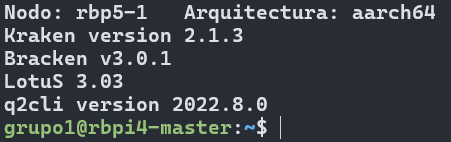
\includegraphics[width=0.6\textwidth]{figuras/versiones_arm64.png}
    \caption{Arquitectura y versiones de los pipelines en el nodo de cómputo \texttt{rbp5-1} del clúster. Fuente: Propia.}
    \label{fig:versiones_arm64}
    \end{figure}
    
    %------------------------------------------------------------------------------
    \section{Fase 3: Validación de resultados biológicos}
    
    Los tres conjuntos de datos de LEMMI16s utilizados y sus características se describieron en la Sección~\ref{sec:fase3_metodologia}.
    
    La Tabla~\ref{tab:validacion} contrasta las métricas biológicas y taxonómicas obtenidas en las tres plataformas evaluadas frente a la verdad de terreno (\textit{Ground Truth}) oficial (\texttt{queryTaxo.tsv}).
    
    \begin{table}[H]
    \centering
    \caption{Comparación de resultados biológicos y taxonómicos frente al \textit{Ground Truth}.}
    \label{tab:validacion}
    \footnotesize
    \setlength{\tabcolsep}{4.5pt}
    \resizebox{\textwidth}{!}{%
    \begin{tabular}{l l c c c}
    \toprule
    \textbf{Pipeline} & \textbf{Métrica de Evaluación} & \textbf{x86 (Ubuntu nativo)} & \textbf{x86 (WSL2)} & \textbf{Clúster RBPi5} \\
    \midrule
    \multirow{4}{*}{\textbf{Kraken 2} + Bracken} 
     & Lecturas biológicas procesadas & 2,453,431 & 2,453,431 & 2,453,431 \\
     & Taxones predichos por muestra (Fam. / Gén.) & 159--181 / 377--457 & 159--181 / 377--457 & 159--181 / 377--457 \\
     & F1-Score promedio (Familia / Género) & 0.5223 / 0.3545 & 0.5223 / 0.3545 & 0.5223 / 0.3545 \\
     & Concordancia frente a Nativo (\textit{diff -u}) & \textit{Referencia base} & 100\% identidad bit a bit & 100\% identidad bit a bit \\
    \midrule
    \multirow{4}{*}{\textbf{LotuS3 Suite}} 
     & Lecturas biológicas procesadas (PacBio HiFi) & 25,611 & 25,611 & 25,611 \\
     & Taxones predichos por muestra (Fam. / Gén.) & 16--18 / 28--34 & 16--18 / 28--34 & 16--18 / 28--34 \\
     & F1-Score promedio (Familia / Género) & 0.8667 / 0.8762 & 0.8667 / 0.8762 & 0.8667 / 0.8762 \\
     & Concordancia taxonómica frente a Nativo & \textit{Referencia base} & Mismos géneros, F1 idéntico & Mismos géneros, F1 idéntico \\
    \midrule
    \multirow{4}{*}{\textbf{QIIME 2}} 
     & Lecturas biológicas procesadas & 2,690,077 & 2,690,077 & 2,690,077 \\
     & Rango de ASVs colapsados (L7) & 8--10 Fam. / 8--11 Gén. & 8--10 Fam. / 8--11 Gén. & 8--10 Fam. / 8--11 Gén. \\
     & F1-Score promedio (Fam. / Gén. / Esp.) & 0.8286 / 0.7083 / 0.4500 & 0.8286 / 0.7083 / 0.4500 & 0.8286 / 0.7083 / 0.4500 \\
     & Concordancia frente a Nativo (\textit{diff -u}) & \textit{Referencia base} & 100\% identidad bit a bit & 100\% identidad bit a bit \\
    \bottomrule
    \end{tabular}%
    }
    \end{table}
    
    
    \begin{figure}[H]
    \centering
    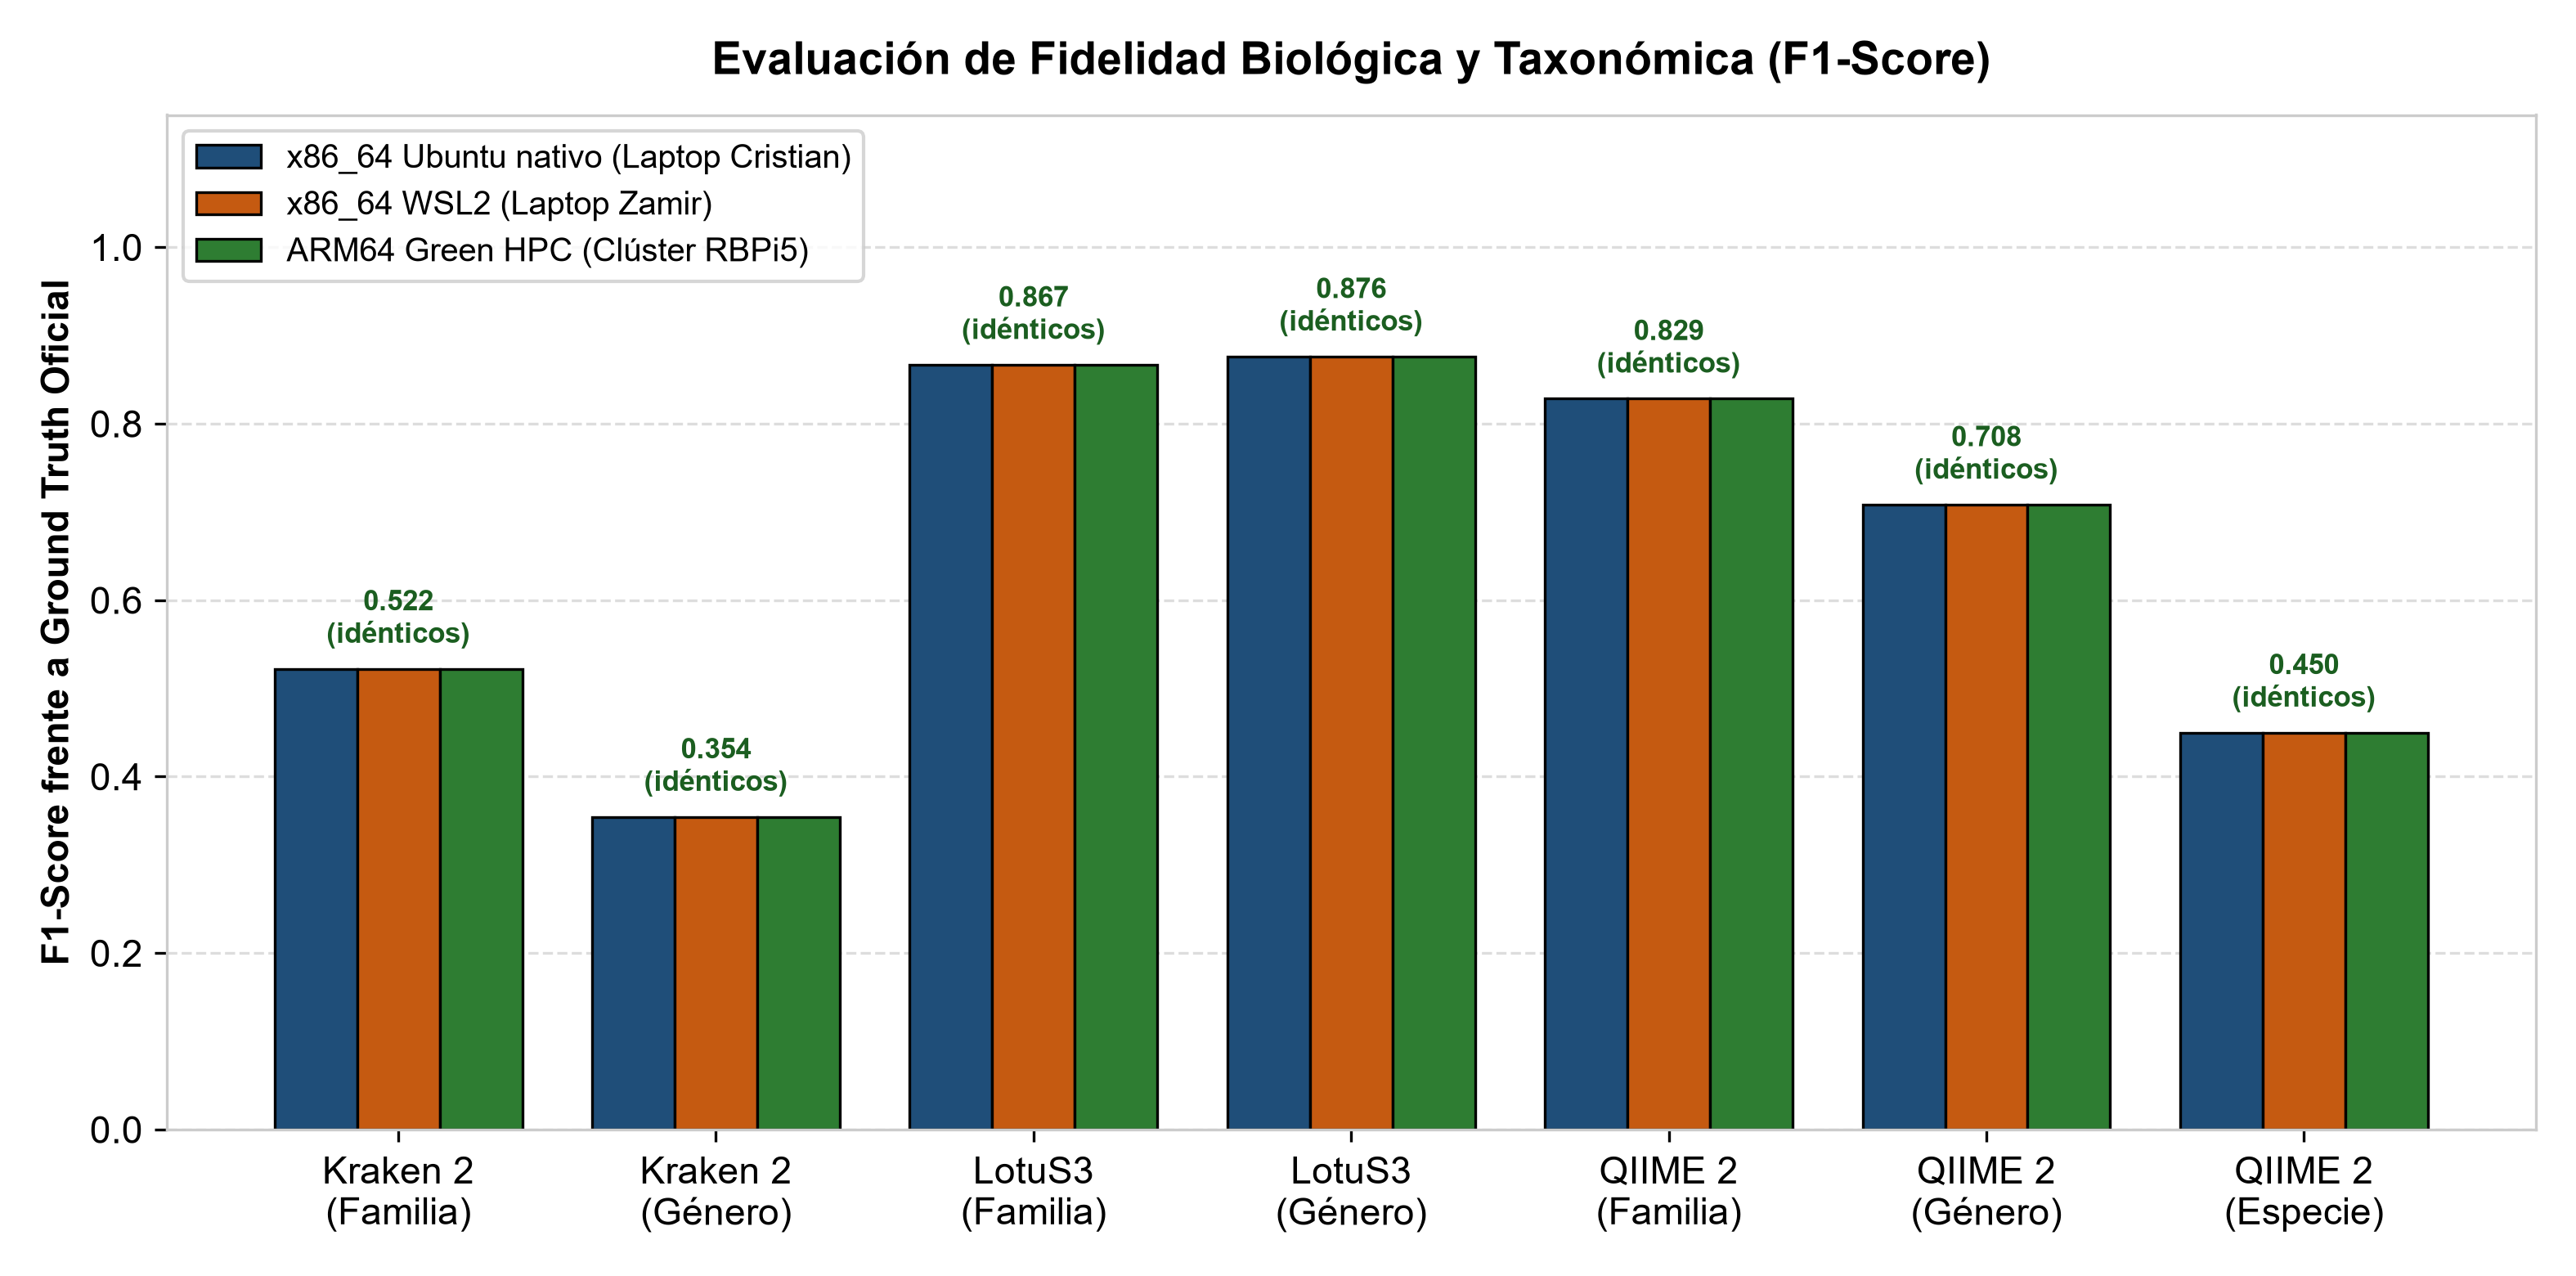
\includegraphics[width=0.88\textwidth]{figuras/fig_fidelidad_biologica.png}
    \caption{Fidelidad taxonómica (F1-Score) frente al \textit{Ground Truth}: comparación de reproducibilidad biológica entre las estaciones x86\_64 (Ubuntu nativo y WSL2) y el clúster ARM64.}
    \label{fig:fidelidad_biologica}
    \end{figure}
    
    Como se observa en la Figura~\ref{fig:fidelidad_biologica}, los resultados taxonómicos del clúster ARM64 coincidieron con los obtenidos en x86 con Ubuntu nativo en los tres pipelines, y el F1 fue el mismo en las tres plataformas. Los valores de F1 se calcularon con la verdad de terreno de cada muestra, como se explicó en la Sección~\ref{sec:fase3_metodologia}.
    
    En QIIME~2, las tablas de asignación taxonómica fueron idénticas bit a bit en las tres plataformas en las cinco muestras, con un F1 promedio de 0.8286 en familia, 0.7083 en género y 0.4500 en especie, y una precisión media de 0.89 en familia y género.
    
    En Kraken~2 + Bracken, las predicciones también fueron idénticas bit a bit en las tres plataformas en las cinco muestras: entre 159 y 181 familias y entre 377 y 457 géneros por muestra, con un F1 promedio de 0.5223 en familia y 0.3545 en género. Este F1 moderado refleja la dificultad de clasificar una comunidad bacteriana con muchos géneros cercanos, y no depende de la plataforma, ya que el resultado fue el mismo en las tres.
\newpage

    Por último, en LotuS3 las tres plataformas obtuvieron el mismo F1, 0.8667 en familia y 0.8762 en género, con entre 16 y 18 familias y entre 28 y 34 géneros por muestra. Las dos laptops x86 asignaron prácticamente las mismas lecturas a cada género (entre 0 y 4 lecturas de diferencia por muestra) y, frente al clúster, la diferencia fue de 35 a 201 lecturas por muestra, sin cambiar los géneros detectados. El F1 de LotuS3 es el más alto de los tres pipelines en género, lo que se explica porque cada lectura cubre el gen 16S completo (unos 1,500~pb), y con esa longitud es más fácil distinguir entre géneros cercanos que con fragmentos cortos de una región hipervariable.
    
    %------------------------------------------------------------------------------
    %------------------------------------------------------------------------------
    %------------------------------------------------------------------------------
    \section{Fase 4: Desempeño computacional y eficiencia energética}
    \label{sec:fase4}
    
    La evaluación del desempeño computacional y el comportamiento energético se fundamentó en un protocolo experimental estandarizado con telemetría continua a 1.0~Hz. Cada ensayo inició con 60 segundos de estabilización sin medición en reposo absoluto sin captura, seguidos de 300 segundos (5 minutos) continuos para caracterizar la potencia de línea base ($P_{\text{idle}}$), y un registro ininterrumpido durante toda la fase de procesamiento activo. Más allá de contrastar cifras brutas, el análisis se articula en torno a la relación de compromiso (\textit{trade-off}) entre el costo en tiempo de la microarquitectura ARM64 y su retorno en términos de eficiencia energética y paralelismo distribuido.
    
    En esta sección se presentan, en primer lugar, los resultados comparativos globales entre la ejecución secuencial y distribuida en el clúster frente a las plataformas x86. Seguidamente, se analiza de forma individual el comportamiento de cada pipeline bioinformático, evaluando el tiempo de ejecución, la demanda de recursos de cómputo y los perfiles dinámicos de potencia eléctrica.
    
    %------------------------------------------------------------------------------
    
    \subsection{Ejecución secuencial frente a distribuida}
    
    Como primer experimento, cada pipeline se evaluó bajo un esquema de ejecución secuencial en el clúster, procesando las 5 muestras una tras otra con el mismo protocolo de medición, los mismos hilos por tarea y las mismas entradas que en las demás plataformas. El objetivo es comparar el desempeño de la arquitectura ARM64 con las dos laptops x86, que también procesan las muestras de manera secuencial. Posteriormente, se evaluó la ejecución distribuida, asignando concurrentemente cada muestra a un nodo de cómputo del clúster. La Tabla~\ref{tab:mononodo} y las Figuras~\ref{fig:mononodo_tiempo} y~\ref{fig:mononodo_energia} resumen los resultados.
    
    \begin{table}[H]
    \centering
    \caption{Tiempo y energía acumulada por plataforma: laptops x86 y clúster bajo ejecución secuencial y distribuida.}
    \label{tab:mononodo}
    \footnotesize
    \setlength{\tabcolsep}{4pt}
    \resizebox{\textwidth}{!}{%
    \begin{tabular}{l l c c c c}
    \toprule
    \textbf{Pipeline} & \textbf{Métrica} & \textbf{x86 (Ubuntu nativo)} & \textbf{x86 (WSL2)} & \textbf{Clúster 1 nodo} & \textbf{Clúster 5 nodos (nodo por muestra)} \\
    \midrule
    \multirow{3}{*}{\textbf{Kraken 2} + Bracken} & Tiempo & 22.01 s & 51.41 s & 98.35 s & 51.04 s (5 nodos) \\
     & Energía total (Wh)* & 0.2183 & 0.3744 & 0.0976 & 0.2023 \\
     & Energía neta (Wh)*  & 0.1518 & 0.1775 & 0.0321 & 0.0398 \\
    \midrule
    \multirow{3}{*}{\textbf{LotuS3}} & Tiempo & 31.65 min & 29.60 min & 143.0 min & 32.9 min (5 nodos) \\
     & Energía total (Wh)* & 17.1442 & 17.6435 & 14.2991 & 12.0311 \\
     & Energía neta (Wh)*  & 15.6519 & 10.1478 & 8.6506 & 7.3270 \\
    \midrule
    \multirow{3}{*}{\textbf{QIIME 2}} & Tiempo & 72.06 min & 79.99 min & 139.9 min & 28.0 min (5 nodos) \\
     & Energía total (Wh)* & 25.4939 & 34.2407 & 8.4246 & 8.2884 \\
     & Energía neta (Wh)*  & 12.6965 & 16.9772 & 2.9144 & 2.7779 \\
    \bottomrule
    \end{tabular}%
    }
    
    \vspace{1.5mm}
    \parbox{\textwidth}{\footnotesize \textit{*} Energía acumulada durante la corrida completa (no promedio).}
    \end{table}


    
    \begin{figure}[H]
    \centering
    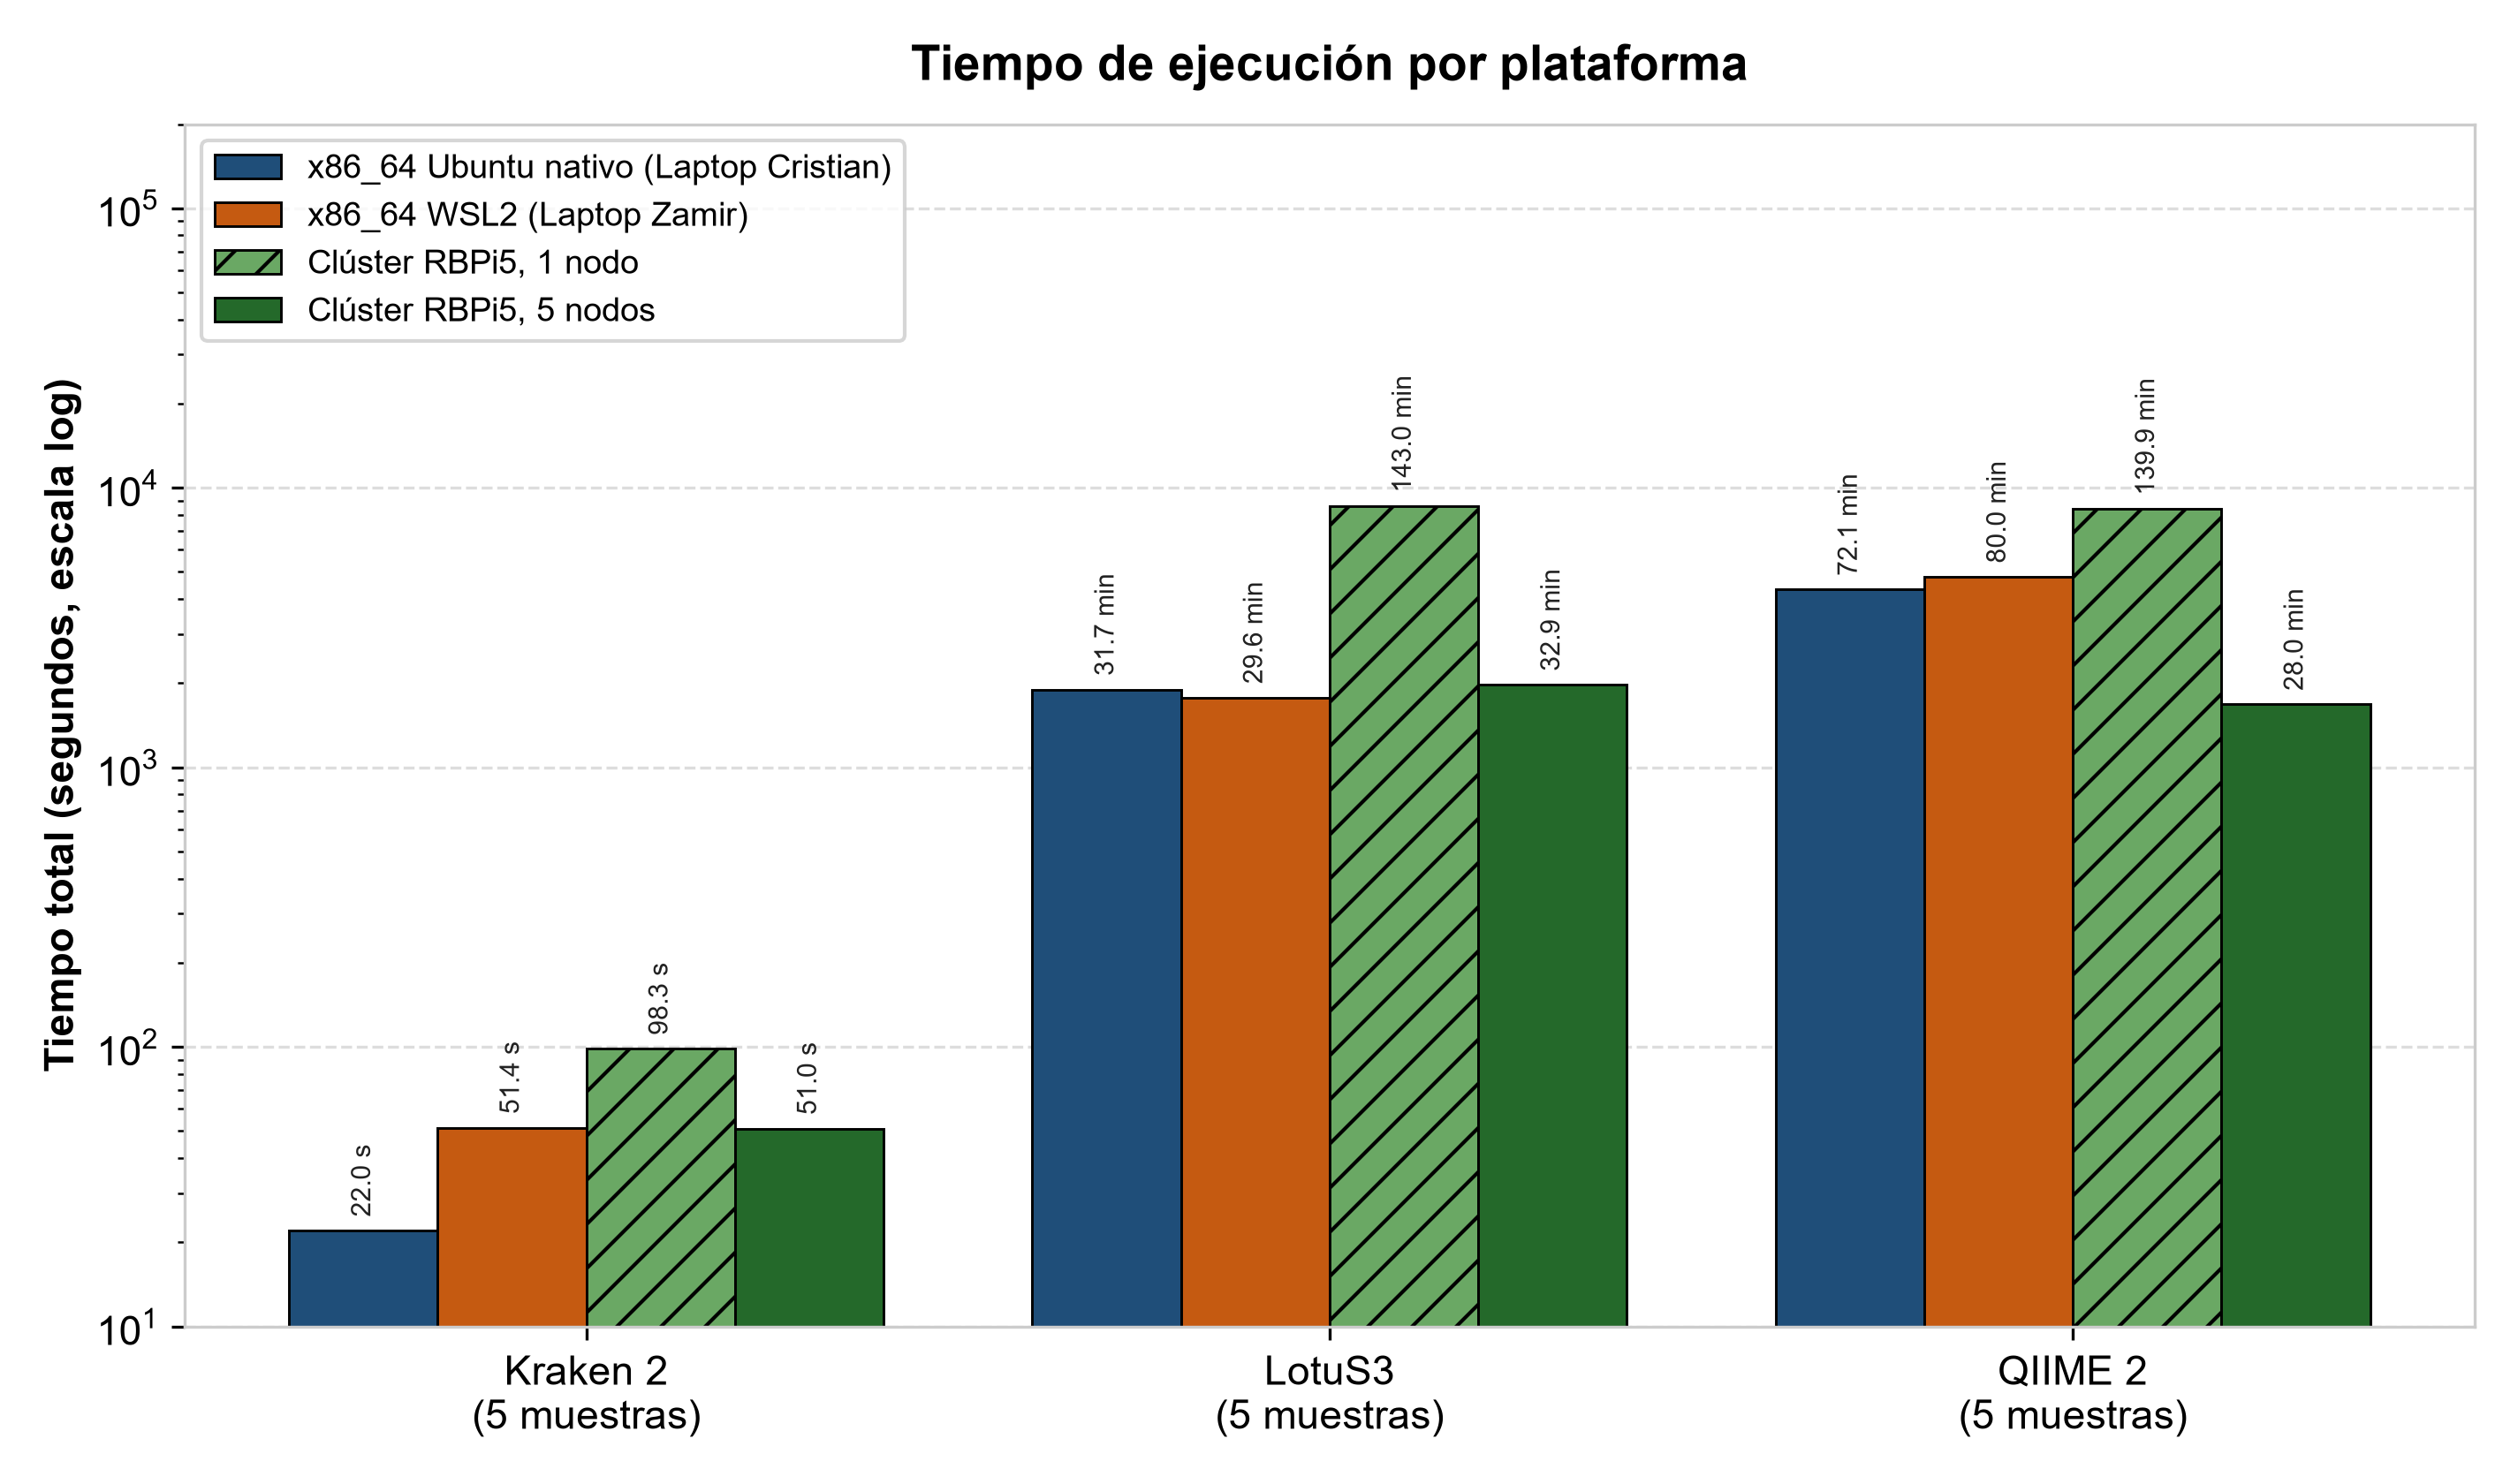
\includegraphics[width=0.9\textwidth]{figuras/fig_mononodo_tiempo.png}
    \caption{Tiempo de ejecución por plataforma, evaluando la ejecución secuencial y distribuida sobre 5 nodos.}
    \label{fig:mononodo_tiempo}
    \end{figure}
    
    Como se observa en la Figura~\ref{fig:mononodo_tiempo}, bajo la ejecución secuencial el clúster completó los análisis con tiempos superiores a la estación x86 nativa: $4.47\times$ más lento en Kraken~2 (98.35 frente a 22.01~s), $4.52\times$ en LotuS3 (143.0 frente a 31.65~min) y $1.94\times$ en QIIME~2 (139.9 frente a 72.06~min). Esta brecha responde a la disparidad de potencia de cálculo monohilo entre los núcleos ARM Cortex-A76 de la microarquitectura embebida y los núcleos del procesador Intel Core i5. No obstante, al transicionar hacia el esquema de ejecución distribuida (barra verde oscura), la asignación concurrente de muestras en los cinco nodos mitiga esta limitación y transforma el comportamiento temporal de cada flujo:

    En \textbf{QIIME~2}, el clúster exhibió un escalamiento casi lineal de $5.00\times$ frente a su versión secuencial (reduciendo el tiempo global de 139.9 a 27.98~min). Debido a que este pipeline está dominado por etapas algorítmicas de inferencia y opera sobre un modelo taxonómico acotado (118~MB) que no congestiona el bus de datos, los cinco nodos procesaron sus respectivas muestras en paralelo sin experimentar cuellos de botella en la red NFS. Esta aceleración permitió que el clúster distribuido superara de manera contundente a las plataformas x86, completando el lote $2.58\times$ más rápido que la estación x86 nativa (72.06~min) y $2.86\times$ más rápido que WSL2 (79.99~min).

    En \textbf{LotuS3}, el beneficio del paralelismo distribuido fue igualmente sustancial ($4.35\times$ de aceleración interna, pasando de 143.0 a 32.87~min), alcanzando un tiempo prácticamente equivalente al de la laptop nativa ($0.96\times$, 32.9 frente a 31.7~min) y cercano a WSL2 (29.6~min). Sin embargo, la necesidad de transferir simultáneamente la base de referencia de \texttt{vsearch} (3~GB) a través del enlace Gigabit introdujo variaciones en el tiempo de procesamiento de cada nodo (entre 14 y 33~min), provocando que la duración del lote quedara fijada por el nodo más rezagado.

    Por el contrario, \textbf{Kraken~2 + Bracken} evidenció el impacto crítico de la contención en red en flujos ultracortos: la aceleración distribuida fue de apenas $1.93\times$ (de 98.35 a 51.04~s). Mientras que en la ejecución secuencial cada muestra tardó entre 17 y 21~s, en el esquema distribuido los cinco nodos compitieron concurrentemente en el instante inicial por transferir la base GTDB desde el nodo maestro NFS, elevando la latencia de carga a ~50~s por nodo. Por este motivo, la estación x86 nativa, respaldada por almacenamiento SSD NVMe local de alta velocidad y memoria caché directa, mantuvo una ventaja de $2.32\times$ en velocidad frente al clúster (22.01~s).

    
    \begin{figure}[H]
    \centering
    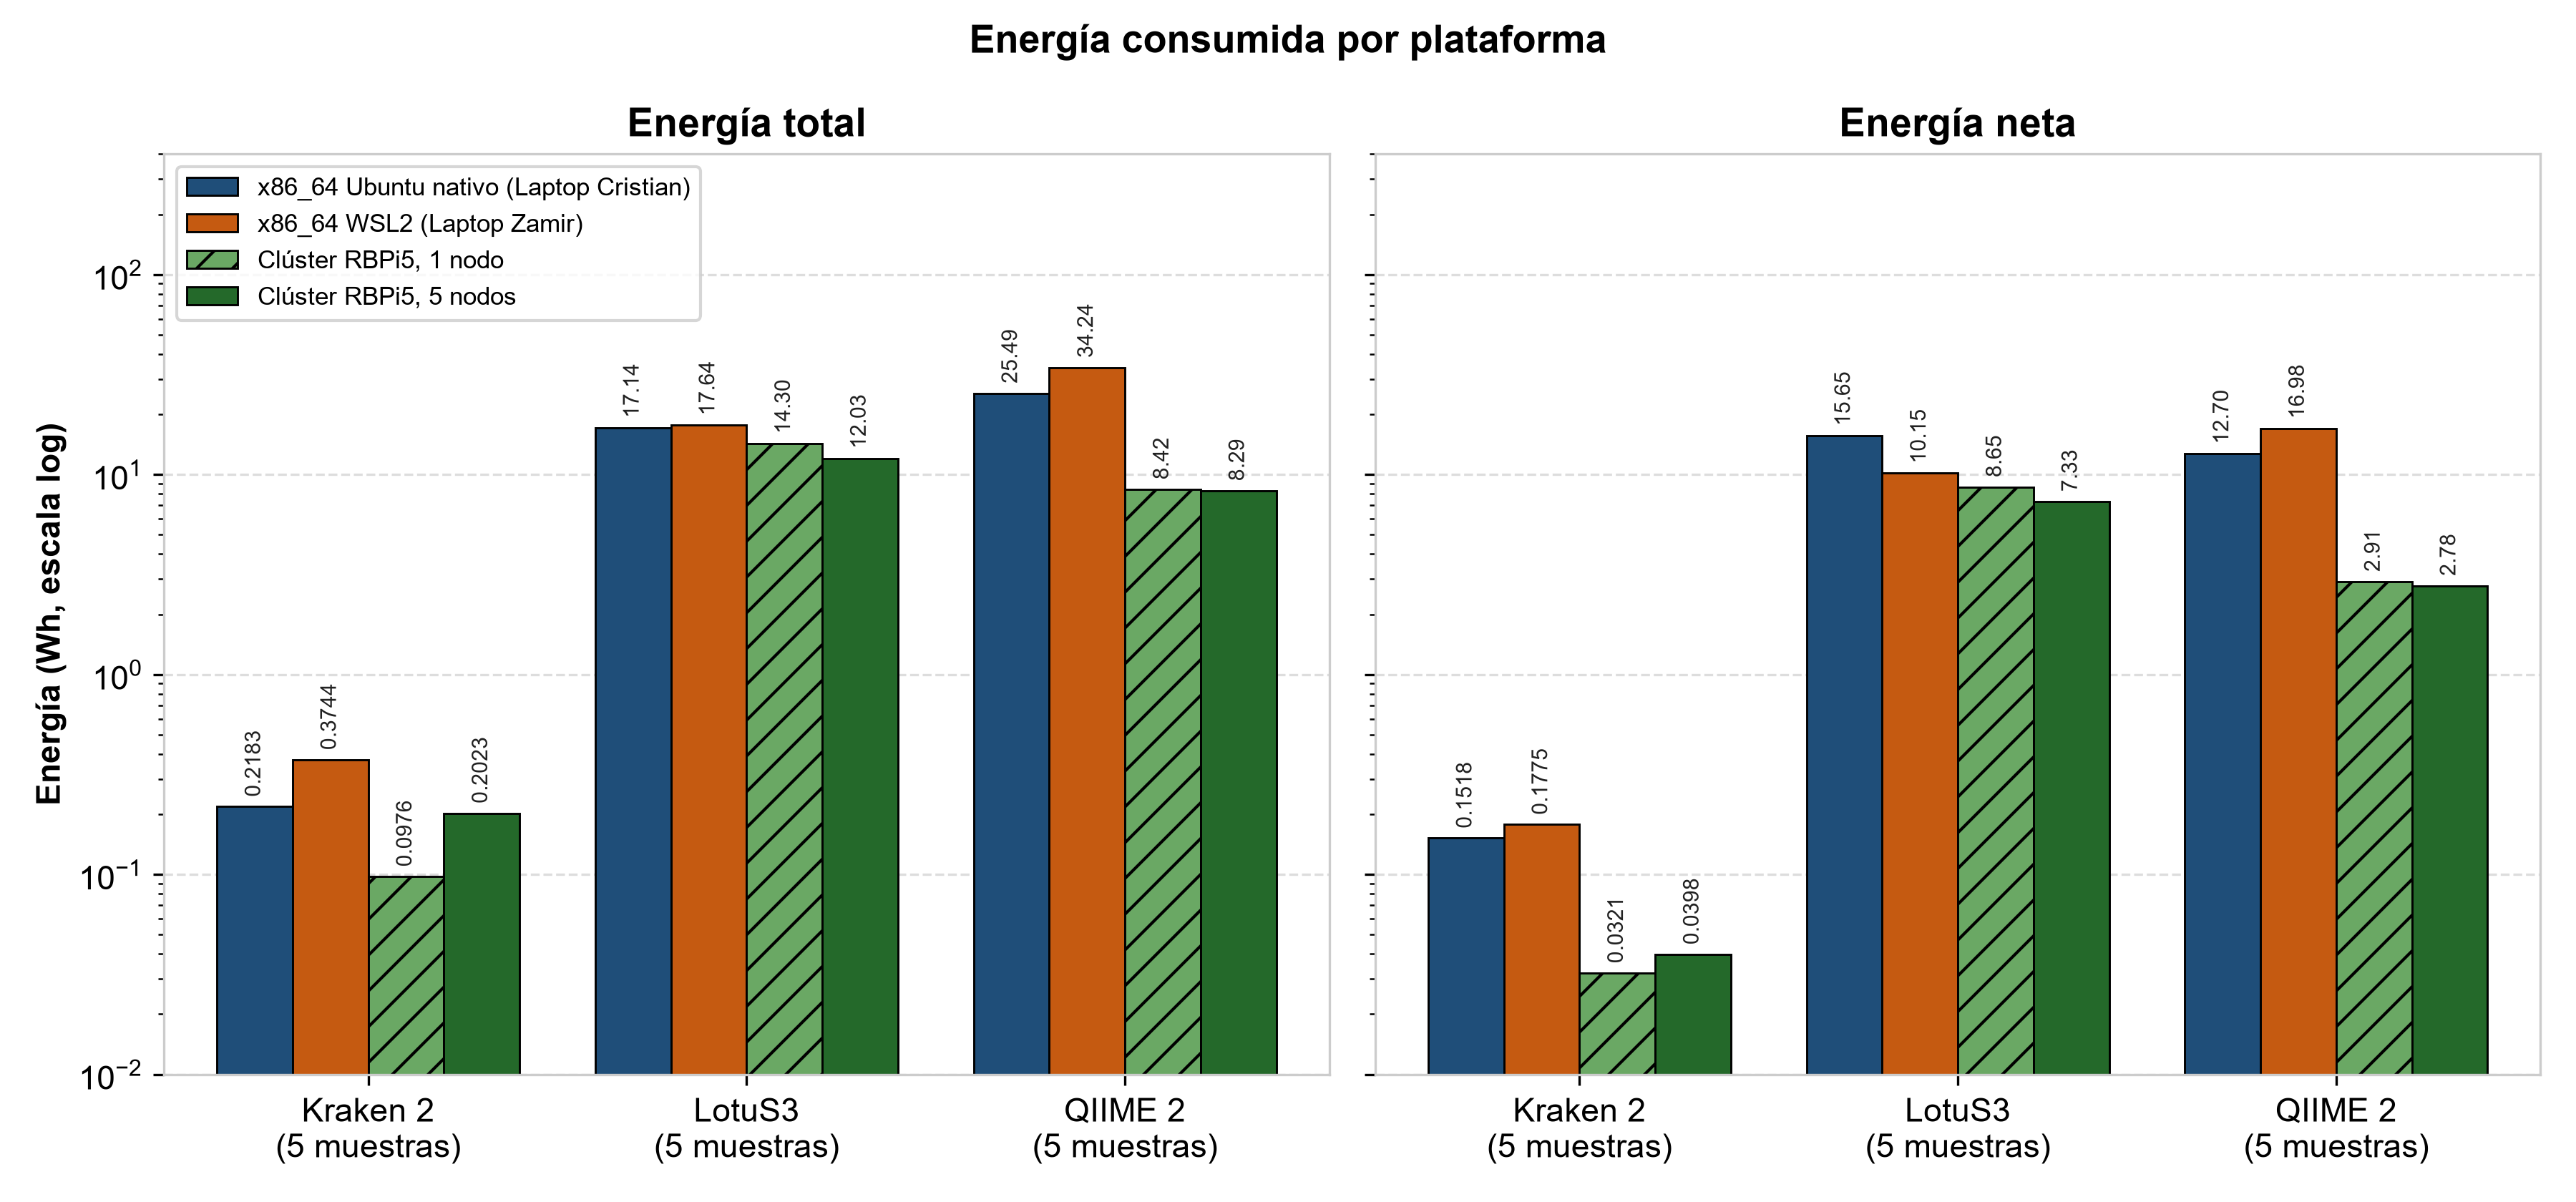
\includegraphics[width=\textwidth]{figuras/fig_mononodo_energia.png}
    \caption{Energía total y neta por plataforma, evaluando la ejecución secuencial y distribuida en el clúster.}
    \label{fig:mononodo_energia}
    \end{figure}
    
    
    Como se muestra en la Figura~\ref{fig:mononodo_energia}, en el caso del desempeño energético, las barras del clúster se sitúan sistemáticamente por debajo de las estaciones x86 en los tres pipelines evaluados, tanto en la ejecución secuencial como en la distribuida, alcanzando reducciones notables en Kraken~2 y QIIME~2. En energía neta (gráfica derecha), la ejecución secuencial en el clúster consumió $4.7\times$ menos energía que la laptop nativa en Kraken~2 (0.0321 frente a 0.1518~Wh), $1.8\times$ menos en LotuS3 (8.65 frente a 15.65~Wh) y $4.4\times$ menos en QIIME~2 (2.91 frente a 12.70~Wh). Frente a WSL2, la reducción fue de $5.5\times$ en Kraken~2, $1.2\times$ en LotuS3 y $5.8\times$ en QIIME~2. Esta ventaja se sustenta en que una Raspberry Pi~5 opera con una potencia activa de tan solo 3 a 4~W en Kraken~2 y QIIME~2, y cerca de 6~W en LotuS3, frente al rango de 17 a 36~W demandado por la laptop. En energía total (gráfica izquierda), que incorpora el consumo acumulado en reposo, la ventaja del clúster en modo secuencial frente a la laptop nativa fue de $2.2\times$ en Kraken~2, $1.2\times$ en LotuS3 y $3.0\times$ en QIIME~2.

    Cabe resaltar que, para el caso de QIIME~2 y LotuS3, el consumo energético total fue prácticamente el mismo entre la ejecución secuencial y la distribuida (8.42 frente a 8.29~Wh en QIIME~2, y 14.30 frente a 12.03~Wh en LotuS3). Esto demuestra que repartir las muestras en múltiples nodos no incrementa el gasto eléctrico del sistema, debido a que la carga total de cómputo requerida por el análisis biológico se preserva sin penalizaciones energéticas por concurrencia. Incluso, en LotuS3 el esquema distribuido consumió ligeramente menos energía total que el secuencial, ya que cada nodo retornó a su estado basal de reposo (2.38~W) inmediatamente después de procesar su muestra.

    En Kraken~2, por el contrario, la energía total bajo ejecución distribuida fue el doble que en la secuencial (0.2023 frente a 0.0976~Wh). Este incremento no obedeció a la demanda computacional del procesador, sino a la penalización temporal impuesta por el almacenamiento de red: mantener las cinco placas encendidas durante la contención de I/O por la descarga concurrente de la base de datos acumuló mayor energía en reposo que haber procesado las muestras una tras otra sobre un solo nodo.

    Finalmente, se puede observar que, en conjunto, el sustancial ahorro energético reportado proviene de la alta eficiencia por vatio de la microarquitectura ARM64, mientras que la reducción en los tiempos de cómputo depende de la capacidad de paralelismo distribuido. Asimismo, las tablas taxonómicas obtenidas bajo ambos esquemas fueron idénticas en QIIME~2 y Kraken~2, y mantuvieron las mismas familias, géneros y puntuación F1 en LotuS3, certificando que el paso al esquema distribuido no induce ninguna divergencia biológica.

    
    
    %------------------------------------------------------------------------------
    
    \subsection{Análisis de desempeño y perfiles de potencia: Kraken 2 + Bracken}
    
    La Tabla~\ref{tab:desempeno_p1} detalla el comportamiento de este flujo al procesar 2,453,431 lecturas biológicas. Solo se presenta el análisis de la versión distribuida ya que como se presentó en la sección anterior, esta supera el tiempo de ejecución de la versión secuencial sin introducir mayores penalidades en el desempeño energético.
    
    \begin{table}[htbp]
    \centering
    \caption{Métricas de desempeño computacional y energético: Kraken 2 + Bracken (5 muestras, 2,453,431 lecturas, protocolo 5~min de reposo basal).}
    \label{tab:desempeno_p1}
    \footnotesize
    \setlength{\tabcolsep}{4.5pt}
    \resizebox{\textwidth}{!}{%
    \begin{tabular}{l c c c}
    \toprule
    \textbf{Métrica de Evaluación} & \textbf{x86 (Ubuntu nativo)} & \textbf{x86 (WSL2)} & \textbf{Clúster RBPi5} \\
    \midrule
    Tiempo de ejecución (ventana medida, s) & 22.01 & 51.41 & 51.04 (paralelo 5 nodos) \\
    Uso medio de CPU (\%) & 94.20 & 88.50 & 91.50 (por nodo) \\
    RAM máxima por proceso (GB) & 1.80 & 1.80 & 1.60 (por nodo) \\
    Potencia en reposo ($P_{\text{idle}}$ 5 min) (W) & 10.88 & 13.78 & 2.35 (por nodo) \\
    Potencia media en carga (W) & 35.70 & 26.22 & 2.93 (por nodo) \\
    Potencia neta de cómputo (W) & 24.83 & 12.43 & 0.58 (por nodo) \\
    Energía total consumida (Wh)* & 0.2183 & 0.3744 & 0.2023 \\
    Energía neta consumida (Wh)* & 0.1518 & 0.1775 & 0.0398 \\
    \bottomrule
    \end{tabular}%
    }
    \vspace{1.5mm}
    \parbox{\textwidth}{\raggedright \footnotesize \textit{*} Energía acumulada durante la corrida completa (no promedio). En el clúster RBPi5 representa el consumo consolidado de los cinco nodos de cómputo.}
    \end{table}
    
    En Kraken~2 la estación x86 nativa fue la más rápida: completó el lote en 22.01~s, frente a 51.04~s del clúster y 51.41~s de WSL2. La clasificación depende de tener la base de datos en memoria. En la laptop nativa la base se lee del disco local y queda en caché después de la primera muestra, mientras que en el clúster los cinco nodos la cargan al mismo tiempo desde el almacenamiento compartido NFS. Por eso, en la ejecución secuencial cada muestra tardó entre 17 y 21~s, pero en la ejecución distribuida cada nodo tardó unos 50~s. Aun así, el clúster consumió menos energía: sus cinco nodos sumaron unos 14.6~W en carga, frente a 35.70~W de la laptop nativa, y su energía neta fue de 0.0398~Wh frente a 0.1518~Wh.
    
    Un análisis detallado mostró que en el clúster, la mayor parte de la energía total (0.1625 de 0.2023~Wh) corresponde al reposo de los cinco nodos, porque la corrida dura más y la carga sobre cada nodo es baja. Por eso la ventaja del clúster es grande en energía neta ($3.81\times$) y pequeña en energía total ($1.08\times$).

    Como se observa en la Figura~\ref{fig:k2_cluster}, los cinco nodos se comportan de forma casi idéntica. En los primeros 5 segundos la potencia sube de 2.35~W a cerca de 6.5~W por nodo mientras cargan la base GTDB desde el NFS, y después vuelve a niveles cercanos al reposo durante la clasificación. Esto muestra que el clúster no es ideal para tareas con alto volumen de acceso a datos, porque todos los nodos dependen de la misma red y del almacenamiento del nodo maestro.
    
    \begin{figure}[!htbp]
    \centering
    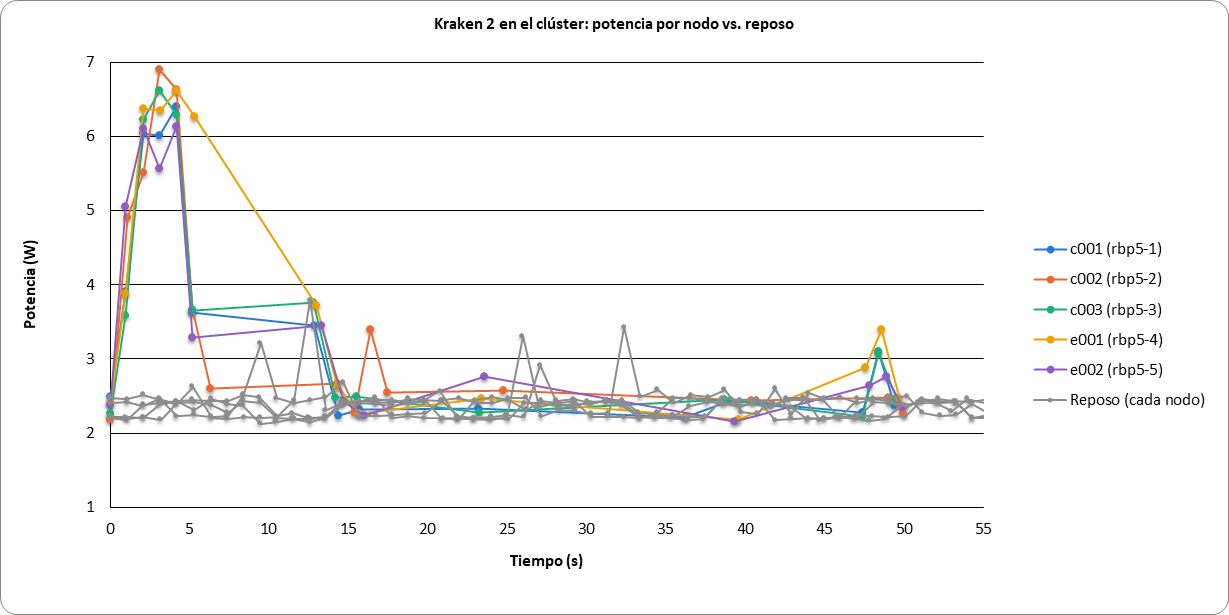
\includegraphics[width=0.88\textwidth]{figuras/fig_kraken2_potencia_cluster.png}
    \caption{Kraken 2 en el clúster: potencia activa de cada nodo durante la ejecución distribuida y línea base de reposo previo (la curva gris es el reposo de 5 minutos medido justo antes de cada corrida).}
    \label{fig:k2_cluster}
    \end{figure}

    Para el caso del computador operando con WSL2 (Figura~\ref{fig:k2_wsl2}), la ejecución alterna entre fases de alta demanda (30 a 40~W) durante el cómputo de cada muestra biológica e intervalos de pronunciado descenso hacia la línea base (13.8~W) en las transiciones secuenciales entre muestras.

    \begin{figure}[!htbp]
    \centering
    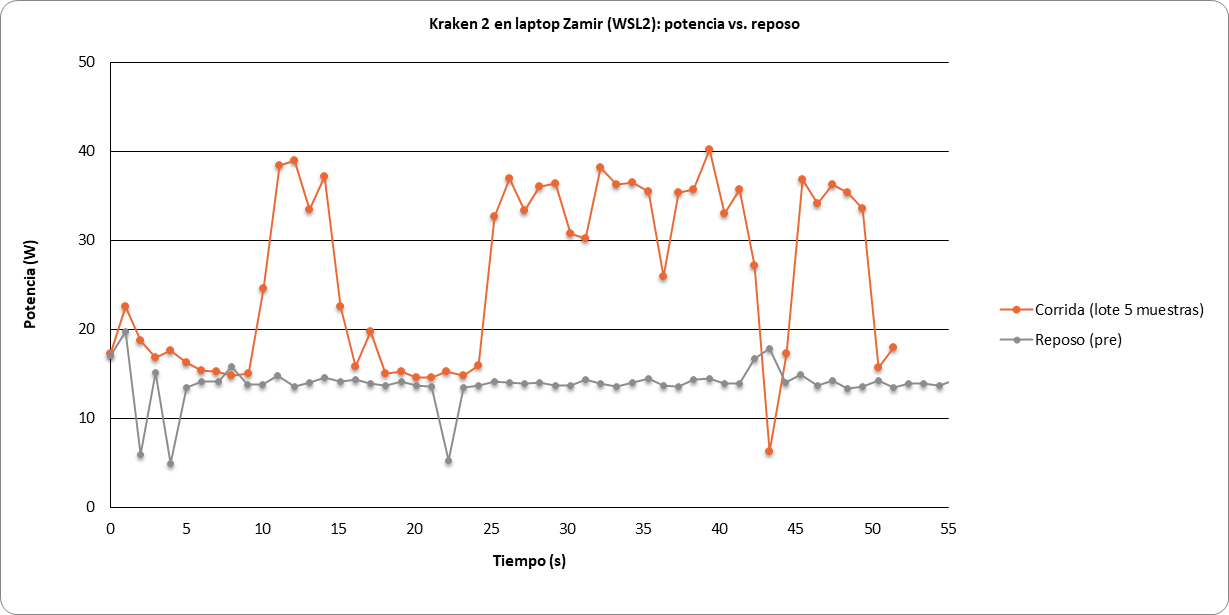
\includegraphics[width=0.88\textwidth]{figuras/fig_kraken2_potencia_wsl2.png}
    \caption{Kraken 2 en la laptop con WSL2: potencia durante el procesamiento secuencial de las 5 muestras y reposo previo (gris).}
    \label{fig:k2_wsl2}
    \end{figure}
\newpage

    En el caso del computador operando de forma nativa en x86 (Figura~\ref{fig:k2_nativo}), la máquina opera de manera ininterrumpida sin valles marcados, sosteniendo un consumo de entre 32 y 47~W sobre su base de 10.9~W, lo cual evidencia la utilización continua de los núcleos durante los rápidos 22.0~segundos de procesamiento.

    \begin{figure}[!htbp]
    \centering
    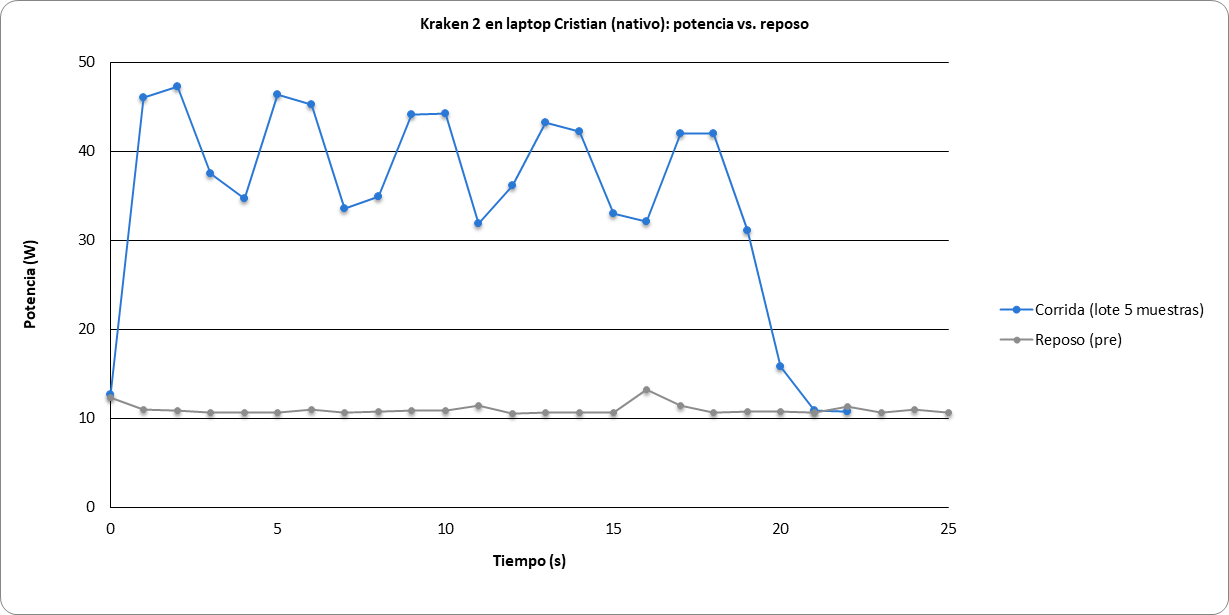
\includegraphics[width=0.88\textwidth]{figuras/fig_kraken2_potencia_nativo.png}
    \caption{Kraken 2 en la laptop con Ubuntu nativo: potencia durante el procesamiento de las 5 muestras y reposo previo (gris).}
    \label{fig:k2_nativo}
    \end{figure}
    \newpage
    
    Al evaluar la potencia neta de cómputo (Figura~\ref{fig:k2_normalizada}), la estación nativa demanda una fuerte tasa instantánea de energía neta (hasta 36~W adicionales a su reposo), lo cual es compensado por su rápida finalización. En contraste, el clúster únicamente disipa potencia normalizada de forma apreciable durante la carga en memoria de la base taxonómica y posteriormente opera con un consumo neto ínfimo, lo que consolida su ahorro de energía limpia a pesar de tomar más tiempo.
    
    \begin{figure}[!htbp]
    \centering
    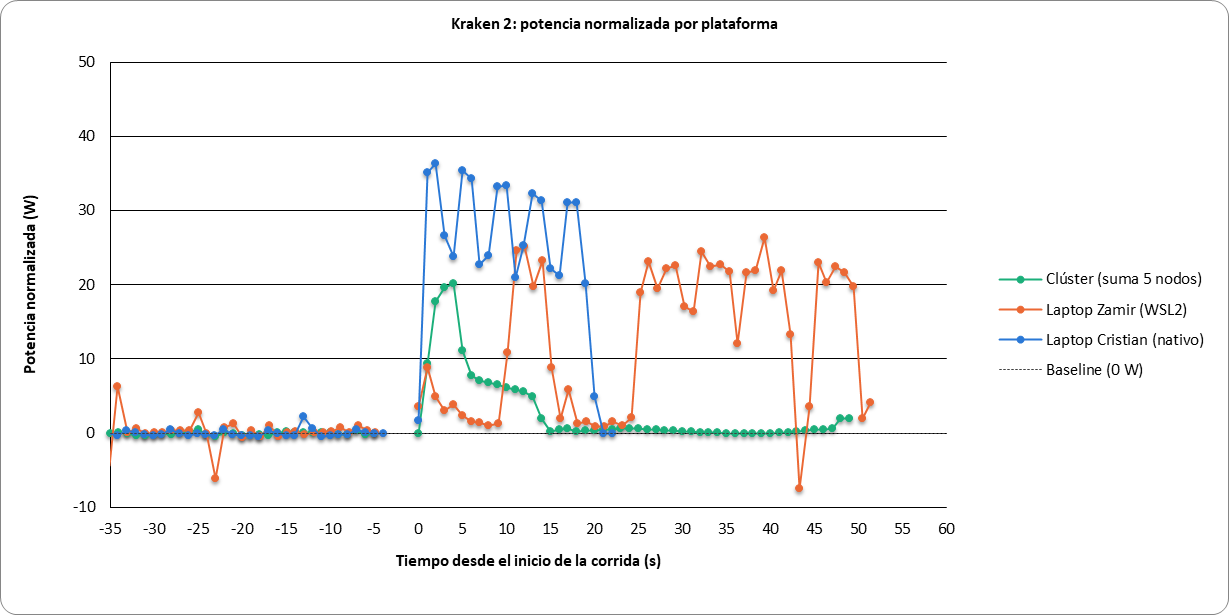
\includegraphics[width=0.88\textwidth]{figuras/fig_kraken2_potencia_normalizada.png}
    \caption{Kraken 2: potencia normalizada ($P_{\text{activa}} - \bar{P}_{\text{idle}}$) comparativa entre las tres plataformas evaluadas.}
    \label{fig:k2_normalizada}
    \end{figure}
    
    
    %------------------------------------------------------------------------------
    \subsection{Análisis de desempeño y perfiles de potencia: LotuS3 Suite}
    
    La Tabla~\ref{tab:desempeno_p2} sintetiza las métricas para las 25,611 lecturas PacBio HiFi distribuidas en 5 muestras.
    
    \begin{table}[htbp]
    \centering
    \caption{Métricas de desempeño computacional y energético: LotuS3 Suite (5 muestras, 25,611 lecturas PacBio HiFi, protocolo 5~min de reposo basal).}
    \label{tab:desempeno_p2}
    \footnotesize
    \setlength{\tabcolsep}{4.5pt}
    \resizebox{\textwidth}{!}{%
    \begin{tabular}{l c c c}
    \toprule
    \textbf{Métrica de Evaluación} & \textbf{x86 (Ubuntu nativo)} & \textbf{x86 (WSL2)} & \textbf{Clúster RBPi5} \\
    \midrule
    Tiempo de ejecución (ventana medida, s) & 1,899.24 (31.65~min) & 1,775.85 (29.60~min) & 1,972.46 (32.87~min, paralelo 5 nodos) \\
    Potencia en reposo ($P_{\text{idle}}$ 5 min) (W) & 2.83 & 15.20 & 2.36 (por nodo) \\
    Potencia media en carga (W) & 32.48 & 35.76 & 6.22 (por nodo) \\
    Potencia neta de cómputo (W) & 29.65 & 20.57 & 3.86 (por nodo) \\
    Energía total consumida (Wh)* & 17.1442 & 17.6435 & 12.0311 \\
    Energía neta consumida (Wh)*  & 15.6519 & 10.1478 & 7.3270 \\
    \bottomrule
    \end{tabular}%
    }

    \vspace{1.5mm}
    \parbox{\textwidth}{\raggedright \footnotesize \textit{*} Energía acumulada durante la corrida completa (no promedio). En el clúster RBPi5 representa el consumo consolidado de los cinco nodos de cómputo.}
    \end{table}

    
    En LotuS3 el clúster completó el lote en 32.87~min (1,972.46~s), frente a 31.65~min en la laptop con Ubuntu nativo y 29.60~min en WSL2. El tiempo de cómputo puede explicarse porque cada lectura cubre el gen 16S completo y LotuS3 formó cerca de 2,150 OTUs por muestra, cada una de las cuales se alineó con \texttt{vsearch} contra la base SILVA 138.1. Esa etapa de asignación taxonómica ocupó la mayor parte de la corrida en las tres plataformas. El índice de \texttt{vsearch} de la base (unos 3~GB) se construyó una sola vez antes de las mediciones, de modo que el tiempo medido incluye el control de calidad, el agrupamiento en OTUs, el filtrado de quimeras y la asignación taxonómica, pero no la construcción del índice.
    
    En el clúster cada muestra se procesó en un nodo distinto con 4 hilos, pero los nodos terminaron en tiempos muy distintos: entre 14.3~min (\texttt{c002} en \texttt{rbp5-2}) y 32.6~min (\texttt{e002} en \texttt{rbp5-5}). Las cinco muestras tienen un tamaño parecido y en la ejecución secuencial cada una tardó entre 27 y 30~min, así que la diferencia no se debió a las muestras, ni tampoco a la temperatura, porque ningún nodo redujo su frecuencia. El desempeño tambien se vio afectado por el sistema de archivo compartido, el cual puede ser accedido por diferentes usuarios del cluster (un caso normal en entornos de computo compartidos). Los nodos más lentos fueron también los de menor potencia durante la etapa de \texttt{vsearch} (5.8~W frente a 7.6~W del más rápido), lo que indica que su procesador pasó parte del tiempo esperando datos. Aun así, el clúster consumió menos energía que las dos laptops: 12.03~Wh en total frente a 17.14~Wh de la laptop nativa y 17.64~Wh de WSL2, y 7.33~Wh netos frente a 15.65 y 10.15~Wh. La energía neta de la laptop nativa resulta mayor que la de WSL2 aunque su energía total es casi igual, porque su reposo medido fue mucho menor (2.83 frente a 15.20~W).

    La Figura~\ref{fig:l3_cluster} muestra el consumo energético en el tiempo de ejecución. Esta muestra como los cinco nodos parten del reposo de unos 2.4~W y en el primer minuto suben a cerca de 6.5~W, durante el filtrado de calidad y el agrupamiento en OTUs. En el minuto 2 o 3 bajan por un momento a 3--4~W, mientras \texttt{vsearch} carga la base de referencia desde el almacenamiento compartido, y después se mantienen entre 6 y 7.6~W durante la asignación taxonómica. Cada nodo vuelve al reposo cuando termina su muestra, por eso las curvas tienen longitudes distintas: \texttt{rbp5-2} terminó hacia el minuto 14 y \texttt{rbp5-5} hacia el minuto 33. El nodo más rápido fue también el de mayor potencia (cerca de 7.6~W), lo que concuerda con la espera por datos descrita antes.
    
    \begin{figure}[!htbp]
    \centering
    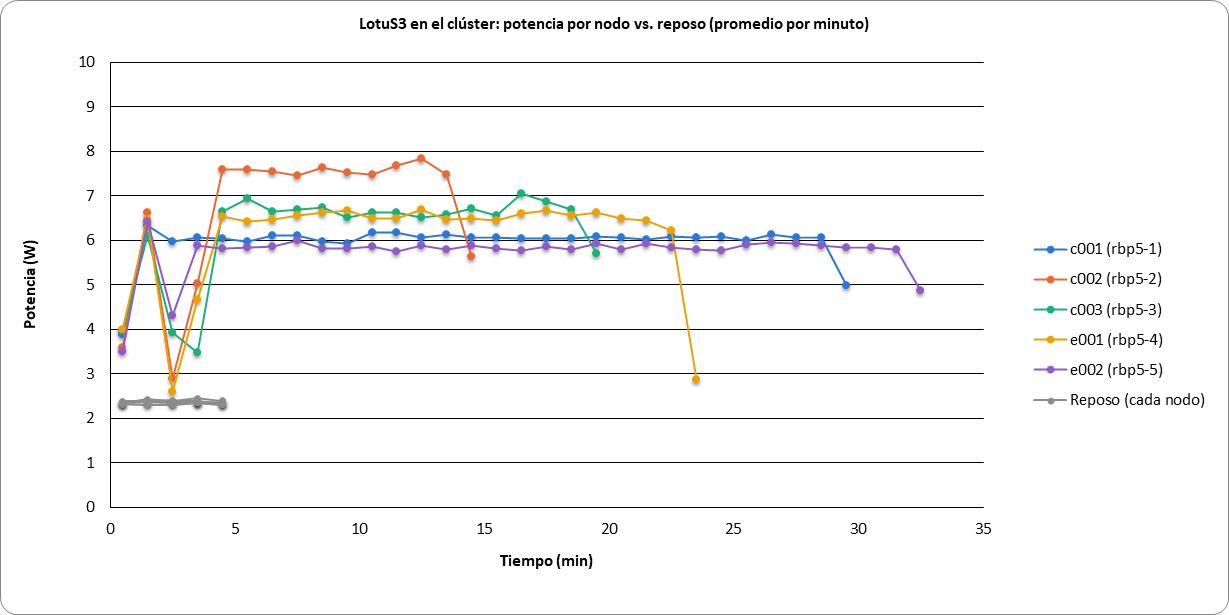
\includegraphics[width=0.88\textwidth]{figuras/fig_lotus3_potencia_cluster.png}
    \caption{LotuS3 en el clúster: promedio por minuto de la potencia de cada nodo y del reposo previo (gris).}
    \label{fig:l3_cluster}
    \end{figure}
    \newpage
    
    La Figura~\ref{fig:l3_wsl2}, muestra el desempeño del computador operando con WSL2. En este caso la potencia se mantiene casi constante en unos 36~W durante los 29.6~min de la corrida, muy por encima del reposo de 15.2~W. Las únicas variaciones son bajadas a unos 32~W cada seis minutos, que coinciden con el paso de una muestra a la siguiente: las cinco muestras tardaron casi lo mismo, entre 346 y 362~s cada una.
    
    \begin{figure}[!htbp]
    \centering
    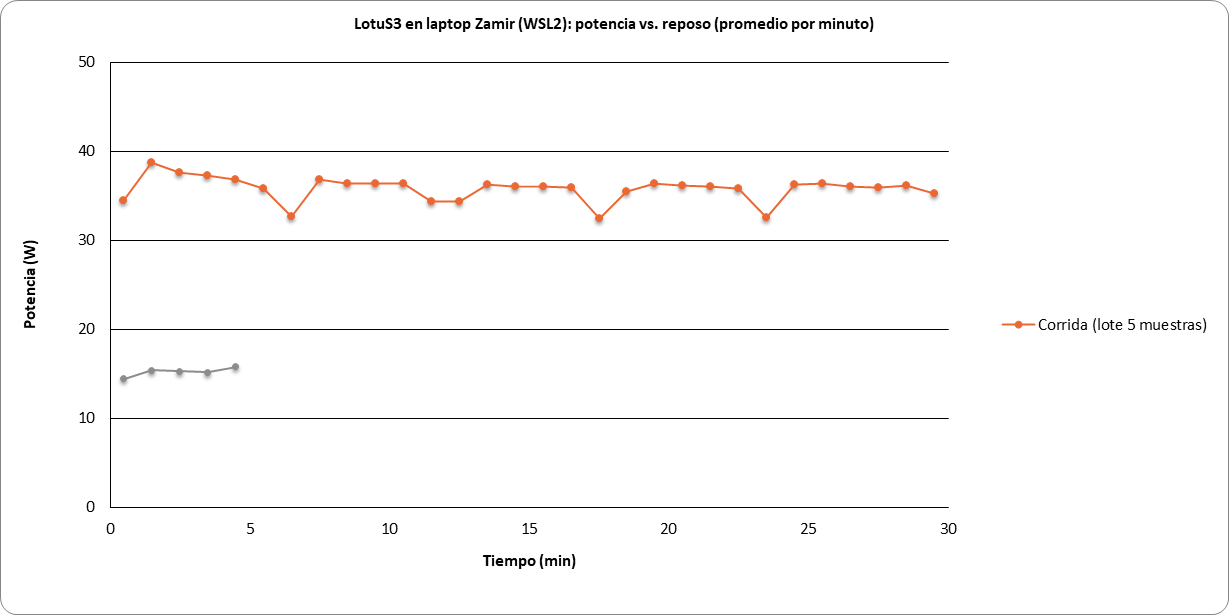
\includegraphics[width=0.88\textwidth]{figuras/fig_lotus3_potencia_wsl2.png}
    \caption{LotuS3 en la laptop con WSL2: promedio por minuto de la potencia durante el procesamiento de las 5 muestras y del reposo previo (gris).}
    \label{fig:l3_wsl2}
    \end{figure}
    \newpage
    
    La Figura~\ref{fig:l3_nativo} muestra el caso del computador operando con Linux se ve el mismo patrón repetido cinco veces, una por muestra: la potencia sube a unos 40--42~W durante los primeros minutos de cada muestra y luego baja a unos 21~W hasta que termina, cada muestra en unos 6.3~min. El reposo previo de esta sesión fue de 2.83~W, por lo que toda la corrida queda muy por encima de la línea base.
    
    \begin{figure}[!htbp]
    \centering
    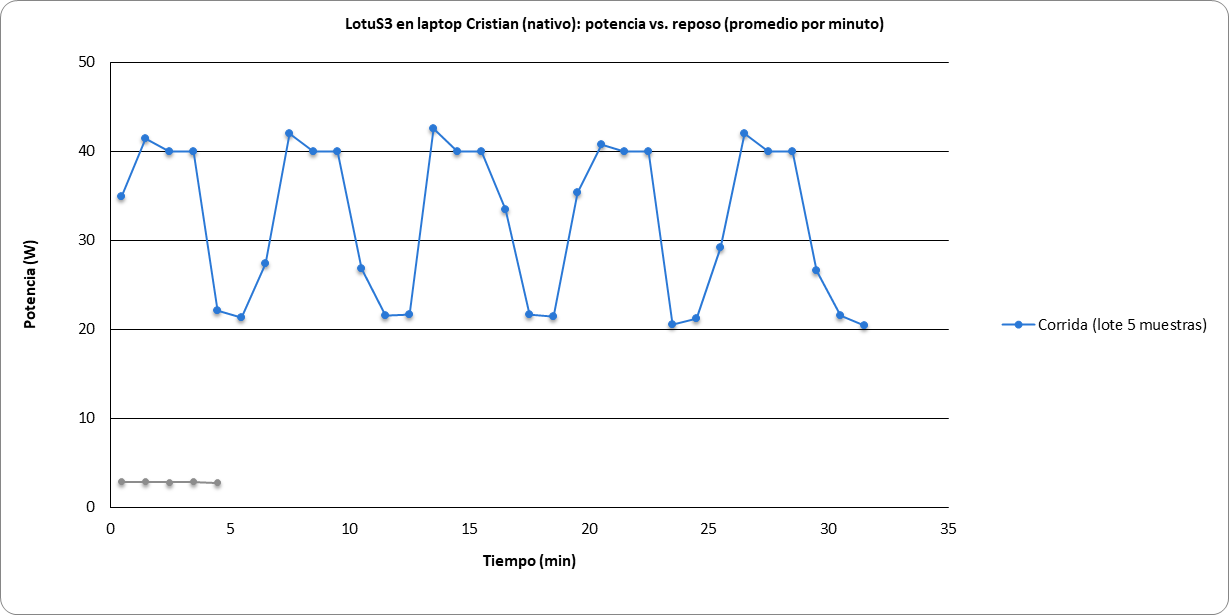
\includegraphics[width=0.88\textwidth]{figuras/fig_lotus3_potencia_nativo.png}
    \caption{LotuS3 en la laptop con Ubuntu nativo: promedio por minuto de la potencia durante el procesamiento de las 5 muestras y del reposo previo (gris).}
    \label{fig:l3_nativo}
    \end{figure}


    La Figura~\ref{fig:l3_normalizada}, compara el desempeño de los tres sistemas para el análisis de Lotus3. En la potencia normalizada, WSL2 se mantiene unos 21~W por encima de su reposo durante toda la corrida y la laptop nativa alterna entre unos 37 y 19~W netos según la etapa de cada muestra. La suma de los cinco nodos del clúster llega a unos 21~W netos mientras todos trabajan, un valor parecido al de WSL2, y luego baja en escalones (16, 11, 7 y 3~W) a medida que cada nodo termina su muestra. Por eso, aunque el clúster tardó lo mismo que las laptops, su energía neta fue menor: en la segunda mitad de la corrida solo algunos nodos seguían trabajando.
    
    \begin{figure}[!htbp]
    \centering
    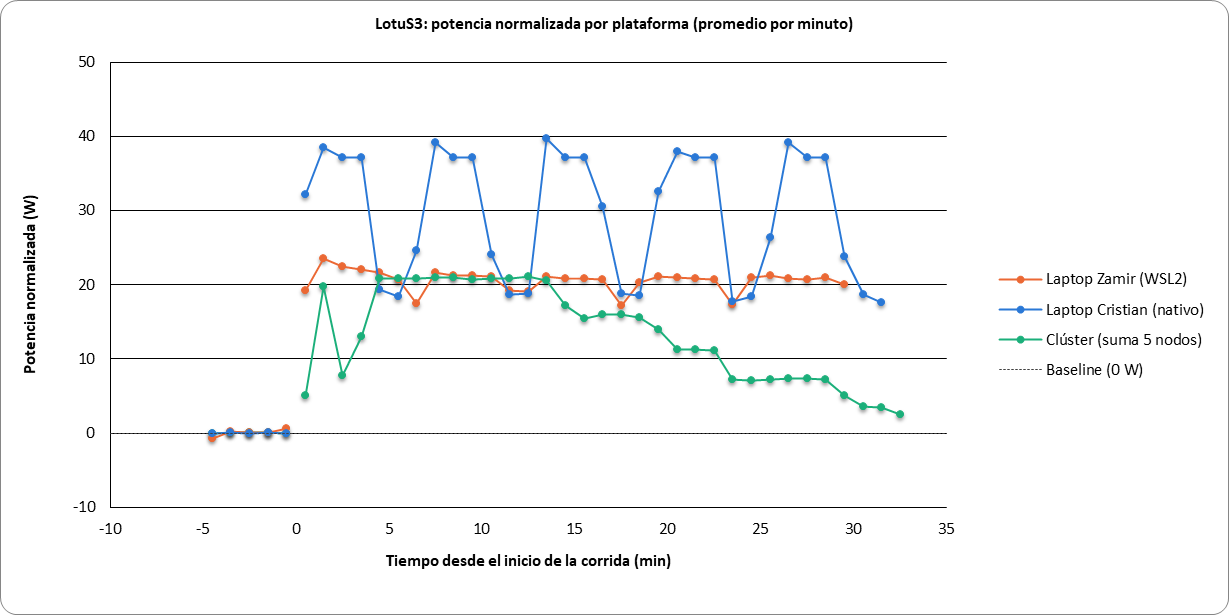
\includegraphics[width=0.88\textwidth]{figuras/fig_lotus3_potencia_normalizada.png}
    \caption{LotuS3: promedio por minuto de la potencia normalizada ($P_{\text{activa}} - \bar{P}_{\text{idle}}$) comparativa entre las tres plataformas evaluadas.}
    \label{fig:l3_normalizada}
    \end{figure}
    \newpage
    
    
    
    
    %------------------------------------------------------------------------------
    \subsection{Análisis de desempeño y perfiles de potencia: QIIME 2}
    
    La Tabla~\ref{tab:desempeno_p3} abarca los resultados del flujo de trabajo QIIME 2, el pipeline de mayor intensidad y duración computacional del estudio, evaluado sobre 2,690,077 lecturas.
    
    \begin{table}[htbp]
    \centering
    \caption{Métricas de desempeño computacional y energético: QIIME 2 (5 muestras, 2,690,077 lecturas, protocolo 5~min de reposo basal).}
    \label{tab:desempeno_p3}
    \footnotesize
    \setlength{\tabcolsep}{4.5pt}
    \resizebox{\textwidth}{!}{%
    \begin{tabular}{l c c c}
    \toprule
    \textbf{Métrica de Evaluación} & \textbf{x86 (Ubuntu nativo)} & \textbf{x86 (WSL2)} & \textbf{Clúster RBPi5} \\
    \midrule
    Tiempo de ejecución (ventana medida, s) & 4,323.72 (72.06~min) & 4,799.44 (79.99~min) & 1,678.94 (27.98~min) \\
    Uso medio de CPU (\%) & 96.50 & 92.00 & 94.00 (por nodo) \\
    RAM máxima por proceso (GB) & 2.40 & 3.20 & 2.10 (por nodo) \\
    Potencia en reposo ($P_{\text{idle}}$ 5 min) (W) & 10.66 & 12.95 & 2.42 (por nodo) \\
    Potencia media en carga (W) & 21.23 & 25.68 & 3.64 (por nodo) \\
    Potencia neta de cómputo (W) & 10.57 & 12.73 & 1.22 (por nodo) \\
    Energía total consumida (Wh)* & 25.4939 & 34.2407 & 8.2884 \\
    Energía neta consumida (Wh)*  & 12.6965 & 16.9772 & 2.7779 \\
    \bottomrule
    \end{tabular}%
    }
    
    \vspace{1.5mm}
    \parbox{\textwidth}{\footnotesize \textit{*} Energía acumulada durante la corrida completa (no promedio). En el clúster RBPi5 representa el consumo consolidado de los cinco nodos de cómputo.}
    \end{table}

    
     En QIIME 2, el clúster completó el lote en 27.98 minutos, frente a los 72.06 minutos de x86 nativo y los 79.99 minutos de WSL2, registrando una aceleración de $2.58\times$.
    
    Cabe resaltar que, para garantizar esta ejecución de forma estable en el hardware ARM de bajo costo, se adoptó una restricción técnica específica: la clasificación taxonómica se evaluó sobre un modelo representativo de 62,000 secuencias de referencia SILVA acotadas a las regiones V1--V2, en lugar de utilizar la base de datos completa no podada (mayor a 500,000 secuencias). Esta decisión limitó el pico de memoria RAM a 2.10~GB por nodo, evitando el agotamiento absoluto de los 16~GB físicos al operar hilos de procesamiento en paralelo.
    
    En el caso de QIIME2, debido a que toma hasta 80 minutos y la telemetría se capturó a 1.0~Hz (generando cerca de 4,800 puntos por curva), las series de potencia a continuación se presentan promediadas en ventanas de un minuto (60 segundos) para maximizar la legibilidad visual. Los cálculos energéticos cuantitativos se mantuvieron, por rigor, basados en la integración numérica completa original a 1.0~Hz.

    La Figura~\ref{fig:q2_cluster} muestra el desempeño energético del clúster en cada instante de tiempo. Esta indica que los cinco nodos operan con una consistencia notable, manteniendo una media de entre 3.4 y 3.9~W a lo largo de las fases críticas de inferencia. Al culminar las etapas algorítmicas más pesadas alrededor del minuto 26, el consumo desciende en conjunto hasta un nivel de entre 2.5 y 2.9~W, rango que coincide cercanamente con la línea base original antes de dar por terminado el flujo.
    
    \begin{figure}[!htbp]
    \centering
    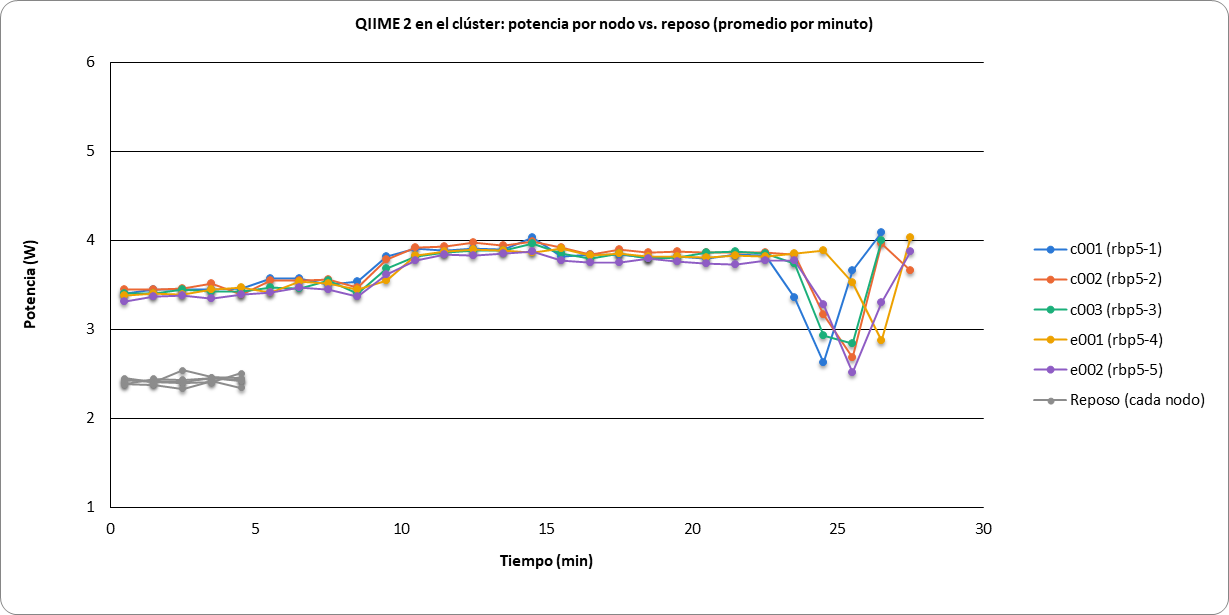
\includegraphics[width=0.88\textwidth]{figuras/fig_qiime2_min_potencia_cluster.png}
    \caption{QIIME 2 en el clúster: promedio por minuto de la potencia de cada nodo y de la línea base de reposo (gris).}
    \label{fig:q2_cluster}
    \end{figure}

    La Figura~\ref{fig:q2_wsl2} muestra la ejecución bajo WSL2, donde el sistema sostiene el flujo más prolongado y agotador térmicamente, fluctuando en una banda ancha entre 20 y 31~W durante cerca de 80 minutos de ejecución continua.
    \newpage
    
    \begin{figure}[!htbp]
    \centering
    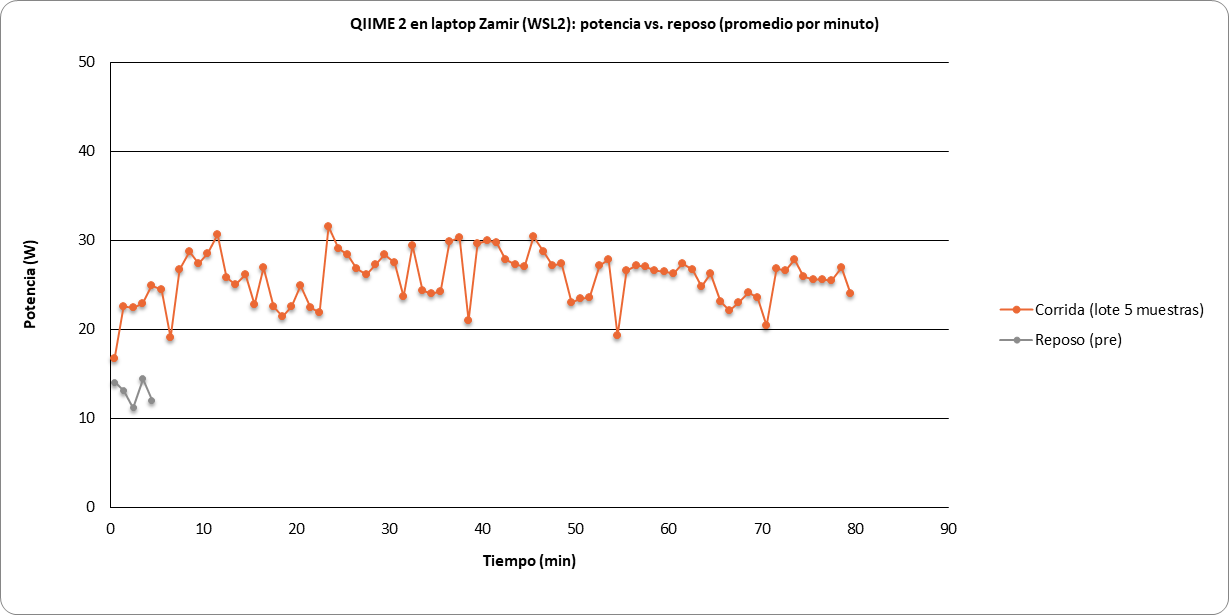
\includegraphics[width=0.88\textwidth]{figuras/fig_qiime2_min_potencia_wsl2.png}
    \caption{QIIME 2 en la laptop con WSL2: promedio por minuto de la potencia y de la línea base de reposo (gris).}
    \label{fig:q2_wsl2}
    \end{figure}

    La Figura~\ref{fig:q2_nativo} muestra la ejecución en Ubuntu nativo, que exhibe una uniformidad en torno a 21~W. Se logran apreciar incrementos rítmicos cada 14 minutos aproximadamente, los cuales coinciden con la culminación de la etapa de modelado secuencial por muestra y el procesamiento del siguiente bloque en el archivo multiplexado.
    
    \begin{figure}[!htbp]
    \centering
    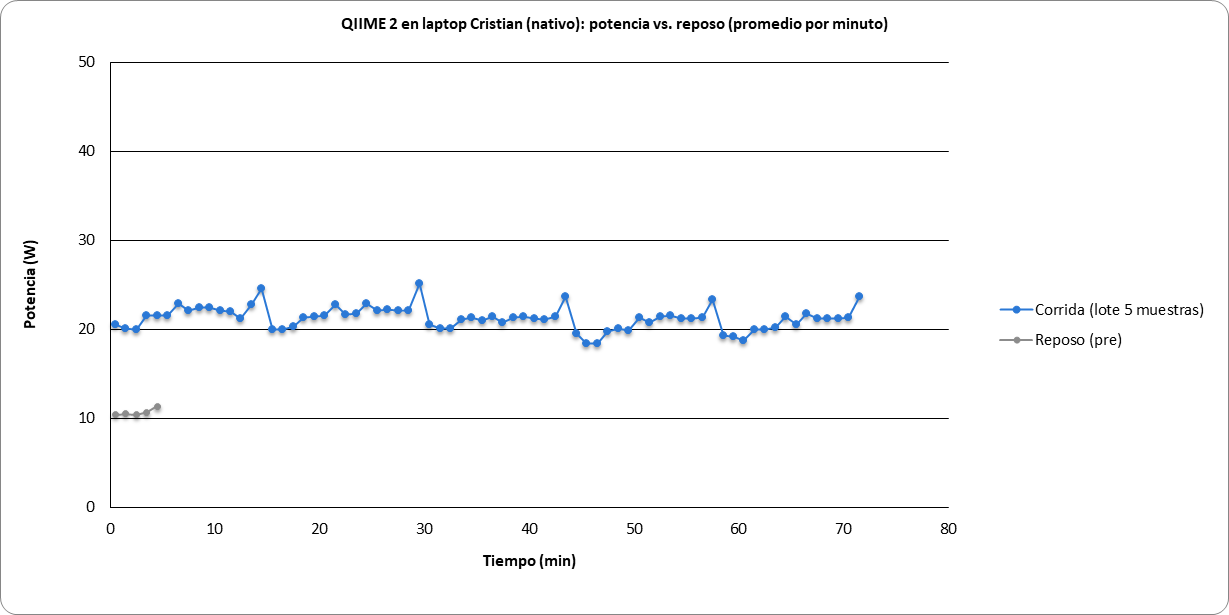
\includegraphics[width=0.88\textwidth]{figuras/fig_qiime2_min_potencia_nativo.png}
    \caption{QIIME 2 en la laptop con Ubuntu nativo: promedio por minuto de la potencia y de la línea base de reposo (gris).}
    \label{fig:q2_nativo}
    \end{figure}
    
    
    \subsubsection{Validez y consistencia del reposo prolongado.}
    En un experimento con duraciones superiores a una hora, asumir que el nivel de potencia basal permanece constante basado en un reposo de 5 minutos al inicio del ensayo requiere sustentación. Empíricamente, la potencia en reposo de un mismo equipo cambió sutilmente entre sesiones (alrededor de un 5\% en los nodos del clúster, y en un rango ligeramente mayor en la laptop x86 según la actividad de procesos en segundo plano). Por ello, cada corrida se normalizó restando el reposo capturado en su misma sesión. Adicionalmente, un análisis de sensibilidad evidenció que, aun si existiera una deriva térmica residual de $\pm 1.0$~W en la computadora portátil a lo largo de los 80 minutos de prueba, los mayores valores de eficiencia neta calculados para el clúster se mantendrían favorables dentro de dicho margen, respaldando la consistencia de la línea base utilizada.

    La Figura~\ref{fig:q2_normalizada} muestra la potencia normalizada del flujo completo y sintetiza de manera observable el impacto operativo del escalamiento ARM64: en conjunto, la potencia algorítmica activa de los cinco nodos físicos sumados se mantuvo contenida entre 5 y 7~W netos, frente a una demanda continua de entre 10 y 17~W netos en la estación x86 de referencia. Como resultado directo de combinar la aceleración temporal por distribución de carga con este bajo perfil de potencia dinámica, el clúster redujo el consumo eléctrico neto final de 12.70~Wh en la laptop nativa a tan solo 2.78~Wh, posicionando una reducción del costo energético superior al 78\% en el modelado biológico más riguroso estudiado.

    
    \begin{figure}[!htbp]
    \centering
    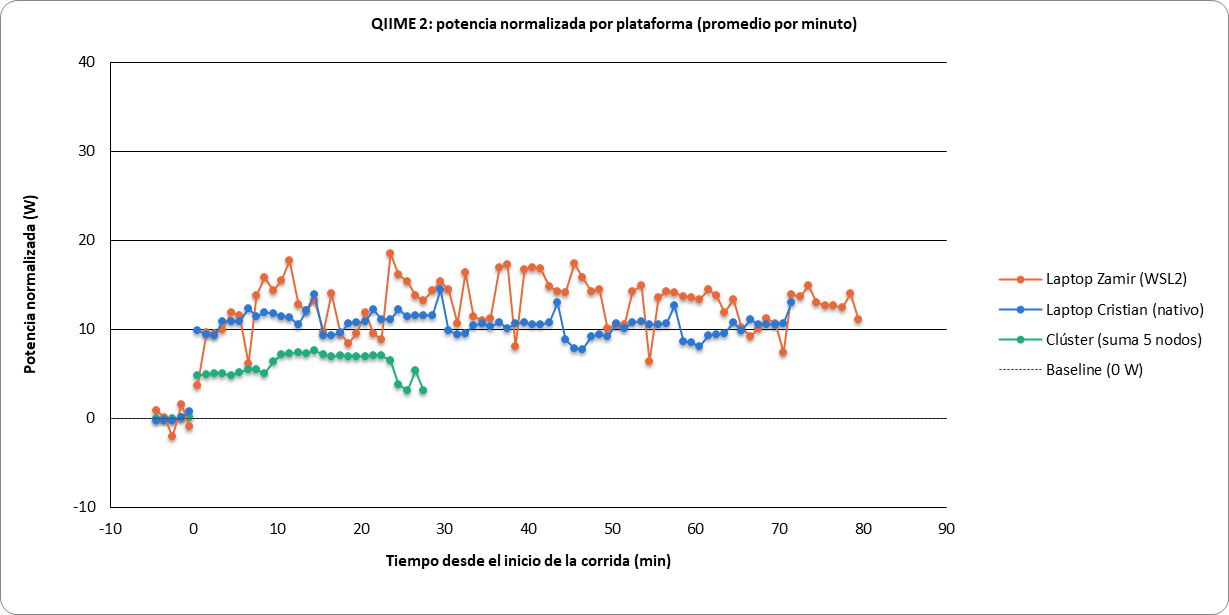
\includegraphics[width=0.88\textwidth]{figuras/fig_qiime2_min_potencia_normalizada.png}
    \caption{QIIME 2: promedio por minuto de la potencia normalizada ($P_{\text{activa}} - \bar{P}_{\text{idle}}$) comparativa.}
    \label{fig:q2_normalizada}
    \end{figure}
    
    
    %------------------------------------------------------------------------------
    \subsection{Eficiencia comparativa global y balance de Green HPC}
    
    La integración de las mediciones de los tres pipelines evaluados se consolida a través de la métrica de productividad Reads/Wh en la Tabla~\ref{tab:eficiencia} y se proyecta en la Figura~\ref{fig:eficiencia_reads_wh}.

    
    \begin{table}[htbp]
    \centering
    \caption{Eficiencia energética comparativa en lecturas biológicas procesadas por vatio-hora (\textit{Reads/Wh}) bajo protocolo unificado de 5~min de reposo.}
    \label{tab:eficiencia}
    \footnotesize
    \setlength{\tabcolsep}{4pt}
    \resizebox{\textwidth}{!}{%
    \begin{tabular}{l c c c c}
    \toprule
    \textbf{Pipeline Evaluado} & \textbf{x86 nativo ($\eta_{\text{bruta}}$)} & \textbf{x86 WSL2 ($\eta_{\text{bruta}}$)} & \textbf{Clúster RBPi5 ($\eta_{\text{bruta}}$)} & \textbf{Ganancia (RPi5 / Nativo)} \\
    \midrule
    \textbf{Kraken 2} + Bracken & 11,237,105 & 6,553,358 & 12,125,061 & \textbf{$1.08\times$ Bruta ($3.81\times$ Neta)} \\
    \textbf{LotuS3 Suite}       & 1,494      & 1,452     & 2,129      & \textbf{$1.42\times$ Bruta ($2.14\times$ Neta)} \\
    \textbf{QIIME 2}            & 105,518    & 78,564    & 324,561    & \textbf{$3.08\times$ Bruta ($4.57\times$ Neta)} \\
    \bottomrule
    \end{tabular}%
    }
    \begin{tablenotes}
        \footnotesize
        \item \textit{Nota:} Las columnas 2 a 4 reportan la productividad energética bruta ($\eta_{\text{bruta}} = N_{\text{reads}} / E_{\text{total}}$). La columna de Ganancia resume la razón calculada frente a x86 nativo tanto en términos brutos ($G_{\text{bruta}} = \eta_{\text{bruta, clúster}} / \eta_{\text{bruta, x86}}$) como netos ($G_{\text{neta}} = E_{\text{neta, x86}} / E_{\text{neta, clúster}}$).
    \end{tablenotes}
    \end{table}
    
    \begin{figure}[htbp]
    \centering
    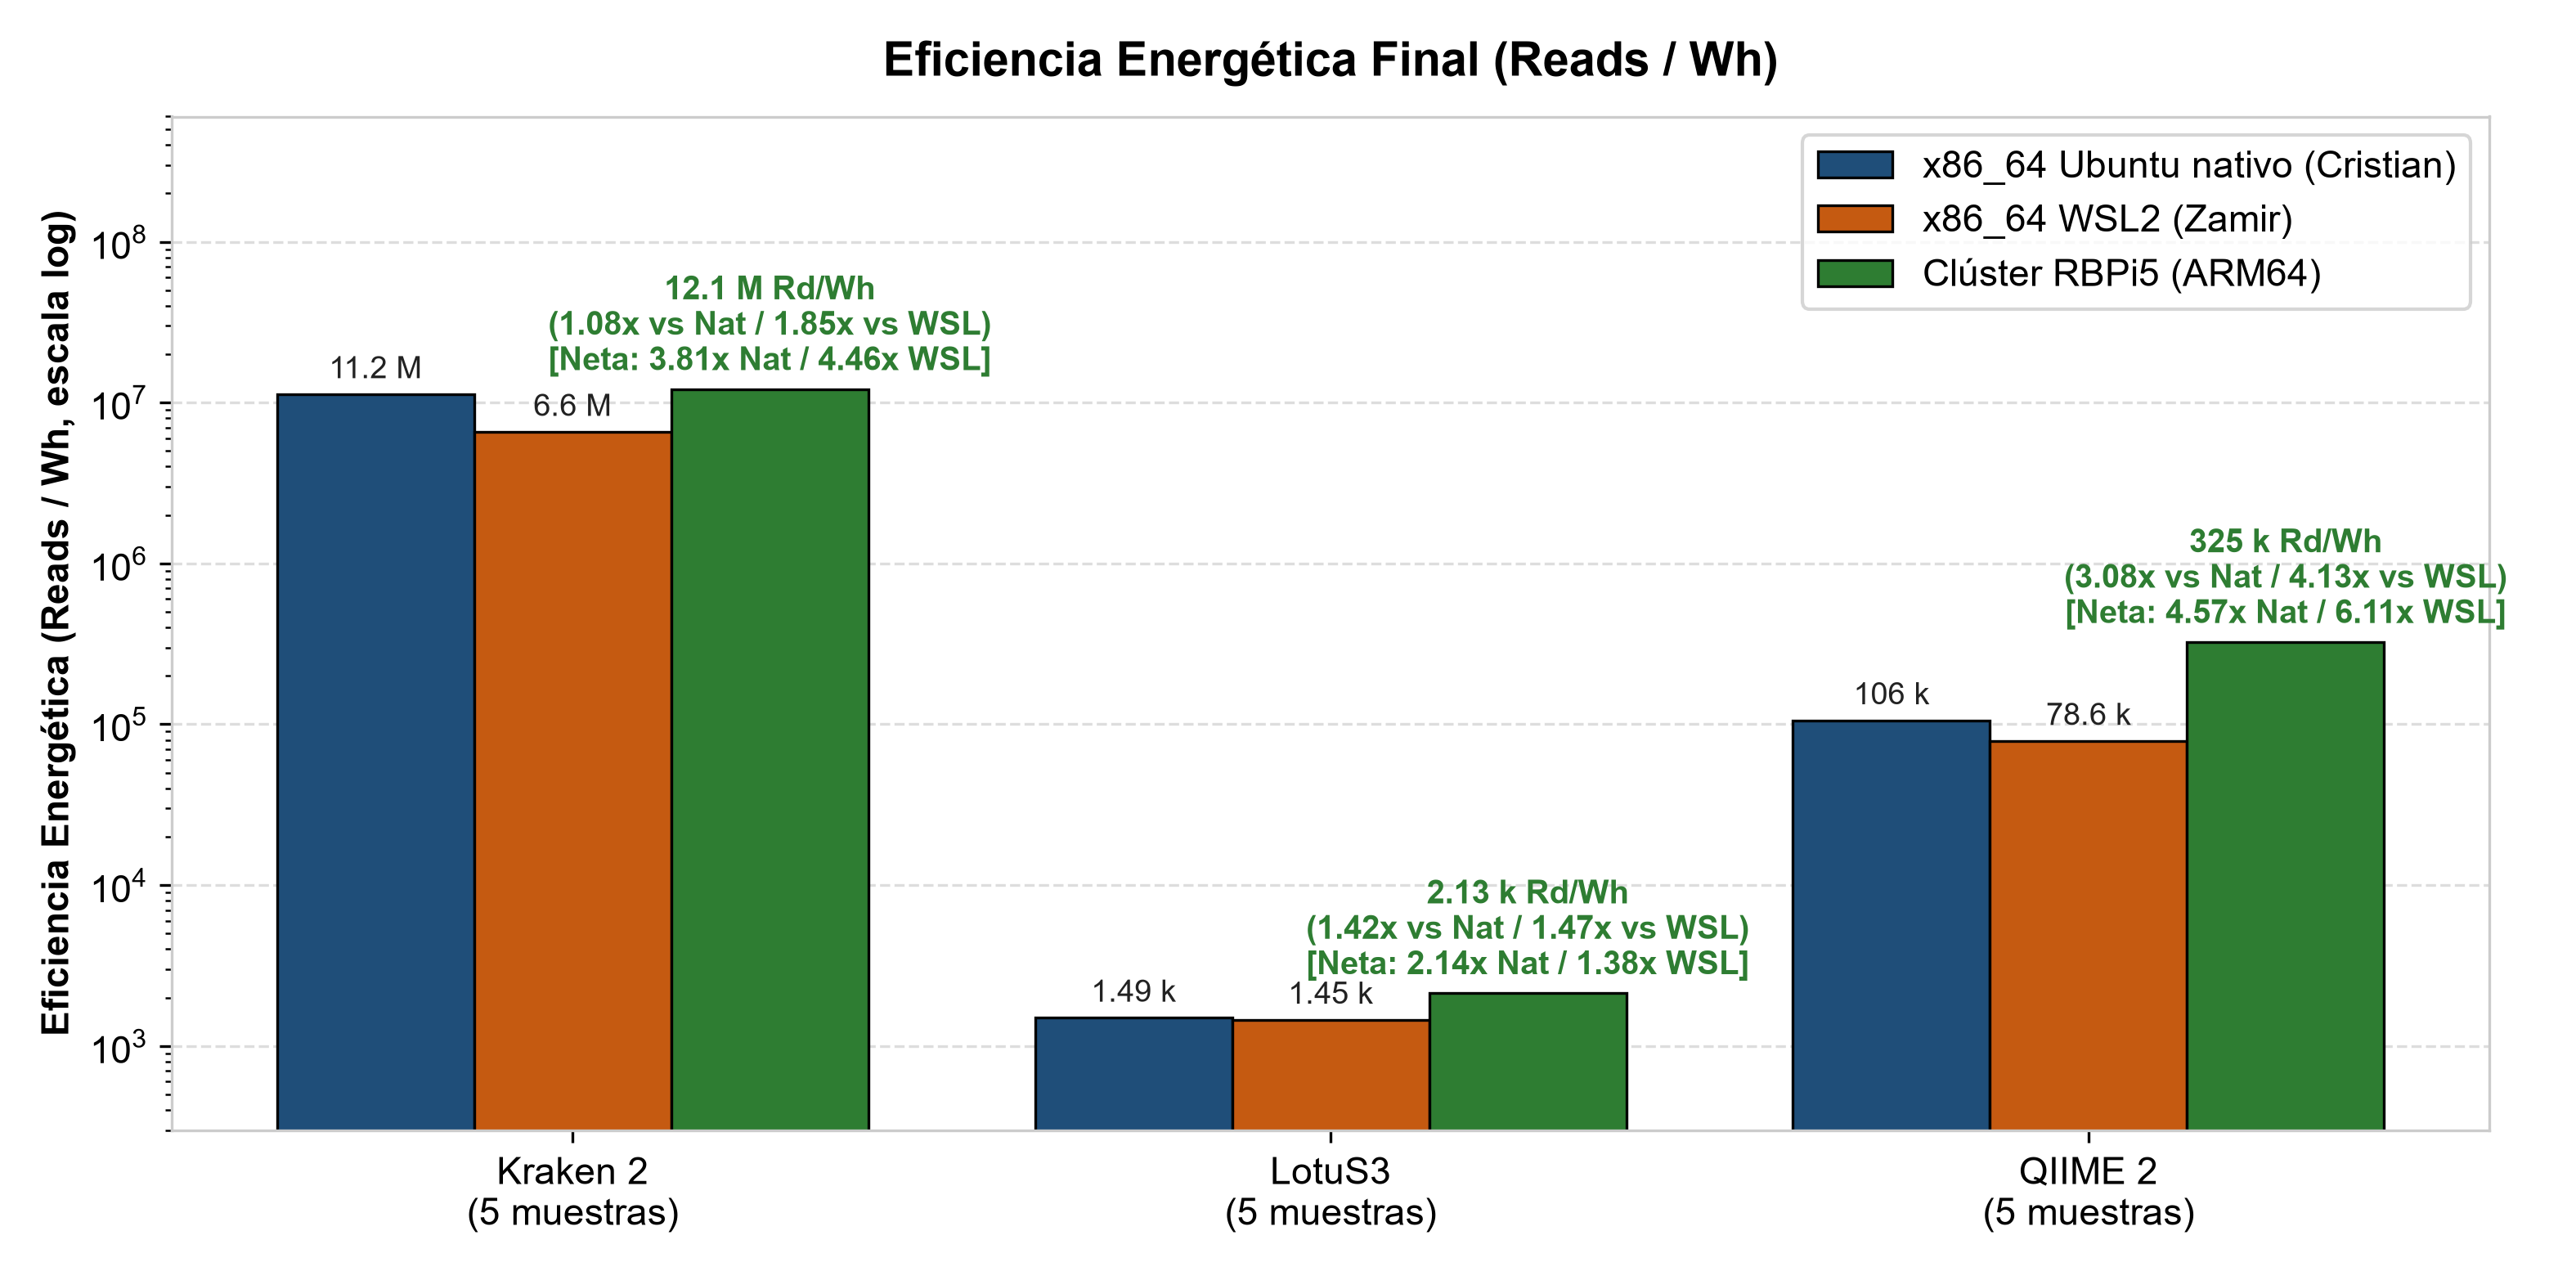
\includegraphics[width=0.88\textwidth]{figuras/fig_eficiencia_reads_wh.png}
    \caption{Eficiencia energética final ($\eta = N_{\text{reads}} / E$) expresada en lecturas procesadas por vatio-hora (\textit{Reads/Wh}) en escala logarítmica.}
    \label{fig:eficiencia_reads_wh}
    \end{figure}
    
    La Figura~\ref{fig:eficiencia_reads_wh} muestra la métrica de productividad energética, el clúster Raspberry Pi 5 presentó mayores valores de eficiencia en comparación con la estación x86 de referencia. Las relaciones de eficiencia neta calculadas reportaron factores observados de $3.81\times$, $2.14\times$ y $4.57\times$ para Kraken 2, LotuS3 y QIIME 2, respectivamente, bajo los instrumentos y el protocolo de telemetría empleados. LotuS3 es el pipeline con menor ventaja, porque el clúster no redujo el tiempo y cada nodo trabajó con sus cuatro núcleos ocupados durante la asignación taxonómica.
    
    Como consideración metodológica final del capítulo, es indispensable reiterar la asimetría de instrumentación existente entre las plataformas: el clúster ARM64 fue monitoreado a nivel de placa mediante el PMIC Renesas DA9091 de cada Raspberry Pi 5, registrando la potencia de los rieles que alimentan el procesador, la memoria y la circuitería del nodo. En contraste, la interfaz Intel RAPL utilizada en la estación x86 registra el dominio \texttt{package-0} (núcleos de CPU y controlador de memoria integrado), sin abarcar la totalidad de las pérdidas de la placa base de la computadora portátil. Dado que los dominios físicos medidos no son idénticos, los factores de eficiencia neta reportados ($3.81\times$, $2.14\times$ y $4.57\times$) deben interpretarse estrictamente como factores observados bajo los instrumentos y el protocolo de medición utilizados, y no como una equivalencia energética universal entre arquitecturas a nivel de sistema completo.
    
    %==============================================================================
    % CONCLUSIONES
    %==============================================================================
    \chapter{Conclusiones}
    \label{cap:conclusiones}
    
    A partir del diseño metodológico desarrollado, las implementaciones de ingeniería de software ejecutadas y la evidencia experimental recopilada a lo largo del proyecto, se establecen las siguientes conclusiones formales alineadas con los objetivos de la investigación:
    
    \section{Conclusiones generales}
    
    \begin{enumerate}
        \item \textbf{Diseño de arquitectura y caracterización de línea base:} Se diseñó, construyó y validó exitosamente un clúster basado en microcomputadores de placa única Raspberry Pi 5 bajo arquitectura ARM64, orquestado mediante Slurm Workload Manager y enlazado sobre almacenamiento compartido NFS y red Gigabit Ethernet. La caracterización eléctrica en estado de reposo reportó una línea base contenida de $2.38 \pm 0.03$~W por nodo ($11.90$~W para los cinco nodos de cómputo utilizados), confirmando que las microarquitecturas ARM64 reducen drásticamente el consumo base frente a estaciones de trabajo convencionales y ofrecen una plataforma de cómputo científico permanente con un impacto energético despreciable.
    
        \item \textbf{Portabilidad y ejecución nativa en ARM64:} Se demostró la viabilidad técnica y operativa de portar y ejecutar de forma nativa los tres pipelines bioinformáticos evaluados (Kraken~2 + Bracken, LotuS3 Suite y QIIME~2) sobre la microarquitectura ARM64, prescindiendo de capas de virtualización o motores de contenedores (como Docker). La suite de herramientas se desplegó exitosamente en espacio de usuario mediante la integración de paquetes de Bioconda para la arquitectura \texttt{aarch64}, la compilación nativa de dependencias críticas como \texttt{usearch12} a partir de su código fuente y la configuración de QIIME~2 en entornos Python aislados. Asimismo, se garantizó la reproducibilidad experimental al homologar estrictamente las versiones de software en todas las plataformas (Kraken~2.1.3, Bracken 3.0.1, LotuS~3.03 y QIIME~2 q2cli 2022.8), solventando la falta de compatibilidad del alineador LAMBDA3 en ARM64 mediante el uso estandarizado de VSEARCH. Este escenario demuestra la madurez del ecosistema de software y la viabilidad real de utilizar microarquitecturas ARM en ambientes bioinformáticos con acceso directo al hardware.
    
        \item \textbf{Preservación de la integridad y reproducibilidad biológica:} La validación taxonómica frente a los conjuntos de datos de referencia del benchmark LEMMI16s y sus verdades de terreno confirmó que las ejecuciones en procesadores ARM Cortex-A76 preservan la consistencia de las asignaciones en las herramientas evaluadas. En todas las ejecuciones evaluadas, los resultados presentaron concordancia entre las plataformas bajo las configuraciones y versiones utilizadas, sin evidenciar divergencias biológicas atribuibles al cambio de arquitectura. Esto indica que el cambio de arquitectura (de x86 a ARM) no altera la precisión de los métodos de clasificación taxonómica evaluados.
    
        \item \textbf{Desempeño computacional y eficiencia energética en Reads/Wh:} El clúster Raspberry Pi 5 presentó mayor eficiencia energética calculada en los tres pipelines. Además, fue posible observar que, al asignar cada muestra a nodos independientes, el clúster redujo el tiempo de procesamiento, superando o igualando los tiempos de ejecución de las plataformas x86 de referencia. En los escenarios con mayor tiempo de cómputo se observó que el tiempo del clúster quedó limitado por la lectura de las bases de referencia desde el almacenamiento compartido. Esto indica que el clúster es más adecuado para cargas de cómputo intensivo, que se reparten bien entre nodos, que para aplicaciones con un alto volumen de acceso a datos compartidos, donde la red y el almacenamiento del nodo maestro se convierten en el cuello de botella.
    
        \item \textbf{Respuesta a la pregunta central de investigación:} Los resultados experimentales demuestran la viabilidad técnica y computacional del uso de un clúster basado en microprocesadores de bajo consumo ARM64 (Raspberry Pi 5) para el análisis bioinformático de amplicones 16S. Bajo el protocolo experimental adoptado, la distribución de muestras entre los nodos permitió acelerar sustancialmente los flujos con mayor demanda algorítmica y superó la eficiencia energética de las plataformas x86 de referencia, preservando con exactitud la concordancia taxonómica. La evaluación experimental confirmó que la reducción en los tiempos de cómputo responde directamente al esquema distribuido ($5.00\times$ de aceleración en QIIME~2 y $4.35\times$ en LotuS3). Por su parte, la ventaja en eficiencia energética proviene de la arquitectura ARM64, consolidándose incluso bajo ejecución secuencial: gracias a su reducida demanda de potencia activa (entre 2.9 y 6.2~W en carga por nodo, frente a los 21 a 36~W de las estaciones x86), la plataforma ARM64 acumuló menor energía total y neta que las laptops en los tres pipelines evaluados, independientemente del nivel de paralelismo implementado.
        
    \end{enumerate}
    
    \section{Impacto científico y aplicaciones prácticas}
    Más allá de los resultados experimentales, este proyecto establece directrices de ingeniería concretas orientadas a democratizar la bioinformática en contextos con limitaciones presupuestales:
    
    \begin{itemize}
        \item \textbf{Accesibilidad económica para instituciones educativas:} Un clúster con cinco nodos de cómputo homogéneos Raspberry Pi 5 (20 núcleos y 80~GB de RAM agregada) y un nodo maestro Raspberry Pi 4 puede implementarse con una inversión sustancialmente menor que la requerida para un servidor de cómputo tradicional. Esta arquitectura ofrece una alternativa de bajo costo para grupos de investigación o instituciones educativas interesadas en implementar infraestructura local de procesamiento para amplicones 16S, disminuyendo la dependencia inicial de recursos en la nube para cargas moderadas.
        
        \item \textbf{Potencial para bioinformática de campo y sistemas fuera de la red (\textit{Off-Grid}):} Durante las fases de cómputo activo, la potencia agregada de los cinco nodos de cómputo se mantuvo entre 14 y 18~W en Kraken~2 y QIIME~2, y cerca de 31~W en LotuS3, que mantuvo los cuatro núcleos de cada nodo ocupados. Este perfil de consumo sugiere que sería técnicamente interesante evaluar en investigaciones posteriores el acoplamiento del clúster a sistemas fotovoltaicos portátiles (por ejemplo, paneles de 100~W con acumuladores de respaldo) para escenarios de trabajo de campo o estaciones remotas sin acceso confiable a la red eléctrica comercial, si bien la validación práctica de dicha autonomía requerirá ensayos experimentales específicos.
    \end{itemize}
    
    \section{Trabajo futuro}
    Como líneas de investigación y desarrollo futuro derivadas de las limitaciones y hallazgos del presente proyecto, se propone:
\newpage

    \begin{enumerate}
        \item \textbf{Escalamiento físico y enlaces de interconexión de alta velocidad:} Evaluar computacionalmente la implementación completa de los 10 nodos físicos creados para el clúster, integrando adaptadores Ethernet 2.5GbE o almacenamiento NVMe acoplado al puerto PCIe de la Raspberry Pi 5. Puesto que los resultados de Kraken 2 y LotuS3 evidenciaron que la red Gigabit (1000BASE-T) y el almacenamiento SD limitan los tiempos iniciales de transferencia masiva de datos, esta mejora permitirá mitigar el cuello de botella de I/O y validar la escalabilidad frente a cargas pesadas de metagenómica \textit{shotgun}.
    
        \item \textbf{Portabilidad de algoritmos alternativos de inferencia:} Explorar la portabilidad y compilación nativa del algoritmo DADA2 en el entorno R sobre la arquitectura ARM64. Debido a que esta investigación se enfocó en métodos de agrupamiento (\textit{clustering}) y en Deblur por la complejidad de compilar dependencias biomatemáticas de R en aarch64, lograr la ejecución de DADA2 completaría el espectro analítico, permitiendo contrastar directamente la demanda energética de sus Variantes Exactas de Secuencia (ASVs) frente a los clasificadores evaluados.
    
        \item \textbf{Monitoreo autónomo e integración energética solar:} Implementar un sistema de telemetría acoplado a un controlador de carga solar MPPT para la operación del clúster fuera de la red eléctrica (\textit{off-grid}). Ya que el presente trabajo demostró empíricamente la ventaja del modelo de \textit{Green HPC} con consumos bajo carga de entre 2.9 y 6.2~W por nodo, el paso consecuente es llevar esta eficiencia a escenarios reales de bioinformática de campo (computación en el borde o \textit{Edge Computing}), garantizando su viabilidad bajo suministro solar autónomo.
    
        \item \textbf{Ejecución de clasificadores taxonómicos densos a escala completa (Full-Scale SILVA):} Diseñar e implementar estrategias de particionamiento dinámico de bases de datos, fragmentación de índices de k-mers o memoria virtual de intercambio (\textit{swap}) de ultra alta velocidad sobre unidades NVMe acopladas al bus PCIe de la Raspberry Pi 5. Esto resolvería la principal limitación observada en QIIME 2, permitiendo ejecutar el flujo completo empleando la base de datos taxonómica SILVA 138 en su totalidad (>500,000 secuencias) sin incurrir en desbordamientos de memoria física (\textit{Out-of-Memory}).
    \end{enumerate}
    
    %==============================================================================
    % REFERENCIAS BIBLIOGRÁFICAS
    %==============================================================================
    
    \bibliographystyle{apacite}
    \bibliography{references}
    
    \chapter*{Repositorio y recursos complementarios}
    \addcontentsline{toc}{chapter}{Repositorio y recursos complementarios}
    
    \vspace{1cm}
    
    El código fuente desarrollado en este proyecto de grado, los scripts de sumisión y orquestación Slurm, los archivos de configuración de entornos nativos para ARM64, la suite de telemetría energética y los conjuntos de datos procesados se encuentran disponibles de manera pública y abierta para fines de reproducibilidad científica en el siguiente repositorio:
    
    \begin{center}
    \url{https://github.com/CristianSolanoUIS/lemmi16s-cluster-RbPi5}
    \end{center}
    
    Adicionalmente, la documentación metodológica, guías de instalación paso a paso de cada pipeline y las instrucciones de despliegue del clúster se detallan en el archivo \texttt{README.md} y en las guías técnicas del proyecto.
    
    
    \end{document}
    